%%% File encoding: UTF-8
%%% äöüÄÖÜß  <-- keine deutschen Umlaute hier? UTF-faehigen Editor verwenden!

\documentclass[bachelor,english]{hgbthesis}
% Zulässige Class Options: 
%   Typ der Arbeit: diplom, master (default), bachelor, praktikum 
%   Hauptsprache: german (default), english
%%%----------------------------------------------------------

\RequirePackage[utf8]{inputenc}		% Bei der Verw. von lualatex oder xelatex entfernen!

\graphicspath{{images/}}    % Abbildungsverzeichnis
\logofile{logo}				% Name des Logo-PDFs in images/ (\logofile{}, wenn kein Logo gewünscht)
\bibliography{literatur}  	% Name der Biblatex-Literaturdatei (.bib)

\usepackage{parskip}		% Absätze
\usepackage{subfigure}		% Bilder nebeneinander
\usepackage{pdfpages}

%%%----------------------------------------------------------
% Angaben für die Titelei (Titelseite, Erklärung etc.)
%%%----------------------------------------------------------

%%% Einträge für ALLE Arbeiten: -----------------------------
\title{Web application development with ReactJS}
\titlefirstline{Web application development}
\titlesecondline{with ReactJS}
\author{Maximilian Zauner}
\versionsnr{6}
\studiengang{Software Engineering}
\studienort{Hagenberg}
\abgabedatum{2017}{05}{31}	% {YYYY}{MM}{DD}

%%% Zusätzlich für eine Bachelorarbeit: ---------------------
\nummer{S1310307115}   % Stud-ID, z.B. 1310238045-A  
% (A = 1. Bachelorarbeit)
\semester{Winter Semester 2016} 
\gegenstand{Software Engineering} 
\betreuer{Dipl. Ing. (FH) Johann Heinzelreiter} % oder \betreuerin{..}

%%% Restriktive Lizenformel anstatt CC (nur für Typ master) -
%\strictlicense

%%%----------------------------------------------------------
\begin{document}
%%%----------------------------------------------------------

%%%----------------------------------------------------------
\frontmatter                    % Titelei (röm. Seitenzahlen)
%%%----------------------------------------------------------

%\maketitle


\includepdf[pages=- , offset=75 -75]{front/Titelblatt_Theoretisch.pdf}

%\chapter{Vorwort} 	% engl. Preface


Dies ist \textbf{Version \hgbthesisDate} der \latex-Dokumentenvorlage für 
verschiedene Abschlussarbeiten an der Fakultät für Informatik, Kommunikation
und Medien der FH Oberösterreich in Hagenberg, die mittlerweile auch 
an anderen Hochschulen im In- und Ausland gerne verwendet wird.

Das Dokument entstand ursprünglich auf Anfragen von Studierenden,
nachdem im Studienjahr 2000/01 erstmals ein offizieller
\latex-Grundkurs im Studiengang Medientechnik und -design an der
FH Hagenberg angeboten wurde. Eigentlich war die Idee, die bereits
bestehende \emph{Word}-Vorlage für Diplomarbeiten "`einfach"' in
\latex\ zu übersetzen und dazu eventuell einige spezielle
Ergänzungen einzubauen. Das erwies sich rasch als wenig
zielführend, da \latex, \va was den Umgang mit Literatur und
Grafiken anbelangt, doch eine wesentlich andere Arbeitsweise
verlangt. Das Ergebnis ist -- von Grund auf neu geschrieben und
wesentlich umfangreicher als das vorherige Dokument --
letztendlich eine Anleitung für das Schreiben mit \latex, ergänzt
mit einigen speziellen (mittlerweile entfernten) Hinweisen für \emph{Word}-Benutzer.
Technische Details zur aktuellen Version finden sich in Anhang \ref{ch:TechnischeInfos}.

Während dieses Dokument anfangs ausschließlich für die Erstellung
von Diplomarbeiten gedacht war, sind nunmehr auch  
\emph{Masterarbeiten}, \emph{Bachelor\-arbeiten} und \emph{Praktikumsberichte} 
abgedeckt, wobei die Unterschiede bewusst gering gehalten wurden.

Bei der Zusammenstellung dieser Vorlage wurde versucht, mit der
Basisfunktionalität von \latex das Auslangen zu finden und -- soweit möglich --
auf zusätzliche Pakete zu verzichten. Das ist nur zum Teil gelungen;
tat\-säch\-lich ist eine Reihe von ergänzenden "`Paketen"' notwendig, wobei jedoch
nur auf gängige Erweiterungen zurückgegriffen wurde.
Selbstverständlich gibt es darüber hinaus eine Vielzahl weiterer Pakete,
die für weitere Verbesserungen und Finessen nützlich sein können. Damit kann
sich aber jeder selbst beschäftigen, sobald das notwendige Selbstvertrauen und
genügend Zeit zum Experimentieren vorhanden sind.
Eine Vielzahl von Details und Tricks sind zwar in diesem Dokument nicht explizit
angeführt, können aber im zugehörigen Quelltext jederzeit ausgeforscht
werden.

Zahlreiche KollegInnen haben durch sorgfältiges Korrekturlesen und
konstruktive Verbesserungsvorschläge wertvolle Unterstützung
geliefert. Speziell bedanken möchte ich mich bei Heinz Dobler für
die konsequente Verbesserung meines "`Computer Slangs"', bei
Elisabeth Mitterbauer für das bewährte orthographische Auge und
bei Wolfgang Hochleitner für die Tests unter Mac~OS.

Die Verwendung dieser Vorlage ist jedermann freigestellt und an
keinerlei Erwähnung gebunden. Allerdings -- wer sie als Grundlage
seiner eigenen Arbeit verwenden möchte, sollte nicht einfach
("`ung'schaut"') darauf los werken, sondern zumindest die
wichtigsten Teile des Dokuments \emph{lesen} und nach Möglichkeit
auch beherzigen. Die Erfahrung zeigt, dass dies die Qualität der
Ergebnisse deutlich zu steigern vermag.

Der Quelltext zu diesem Dokument sowie das zugehörige
\latex-Paket sind in der jeweils aktuellen Version online
verfügbar unter
%
\begin{itemize}
\item[]\url{https://sourceforge.net/projects/hgbthesis/}.
\end{itemize}
%
Trotz großer Mühe enthält dieses Dokument zweifellos Fehler und Unzulänglichkeiten
-- Kommentare, Verbesserungsvorschläge und passende Ergänzungen
sind daher stets willkommen, am einfachsten per E-Mail direkt an mich:
\begin{itemize}
\item[]%

Dr.\ Wilhelm Burger, Department für Digitale Medien,\newline
Fachhochschule Oberösterreich, Campus Hagenberg (Österreich)\newline
\nolinkurl{wilhelm.burger@fh-hagenberg.at}
\end{itemize}

\noindent
Übrigens, hier im Vorwort (das bei Diplom- und Masterarbeiten üblich, bei Bachelorarbeiten 
aber entbehrlich ist) kann kurz auf die Entstehung des Dokuments eingegangen werden.
Hier ist auch der Platz für allfällige Danksagungen (\zB an den Betreuer, 
den Begutachter, die Familie, den Hund, \ldots), Widmungen und philosophische 
Anmerkungen. Das sollte allerdings auch nicht übertrieben werden und sich auf 
einen Umfang von maximal zwei Seiten beschränken.




 % Optional. Ggf. weglassen	
%\chapter*{Abstract}

The goal of this thesis is to provide an overview to web application development with JavaScript by using Facebook's front end framework ReactJS. It is directed at developers that would like to start developing web application software in general or at intermediate web developers who want to get started with ReactJS. 

%The reader should have a basic understanding of general software development in order to being able to understand all explanations and discussions that are provided in this thesis.

However, the emphasis is on raising attention that application architecture and a well structured code base is one of the most important aspects of any web application software project. Currently many software projects exist in the web that are hardly maintainable and have a bad or no application architecture at all which obviously leads to problems when the project has to be maintained over a longer time period.

The research section of this thesis is about the comparison between the application architecture paradigm called Flux which was invented by Facebook and the traditional Model View Controller (MVC) pattern. After research it is shown that the Flux pattern is very similar to the MVC pattern but still viable to be used in web application software projects.

On top of a broad introduction to the general JavaSript ecosystem and all of its tooling that is necessary to get started, this thesis also gives a specific introduction to the ReactJS library itself. It thus comprises a concise summary of all requirements and best practices of developing a web application with ReactJS.

As part of this work a prototype for a web application with ReactJS was developed and is introduced to the user. The research that is presented in this thesis is further corroborated by studying a real world example.


%Nowadays the modern web developer uses JavaScript front end libraries like ReactJS, Angular2 or VueJS for creating web applications. Oftentimes it is very difficult to decide what framework to use. Even though the same goal is achieved with all libraries, the frameworks use different software paradigms and use different approaches to solve software architectural problems. This fact makes some libraries fit better in certain situations than  others. The key is to get a rough understanding of all the different libraries and their approaches to solve problems to be able to decide what framework fits best in what problem statement.

%\today 

%This paper not only provides an overview to the JavaScript front end framework ReactJS but also introduces the reader to a new software paradigm called Flux

%as time progresses all get more similarasdfa

			
%\chapter*{Kurzfassung}

Diese Arbeit gibt einen Überblick über die Enwicklung von Webanwendungen mit dem JavaScript Framework ReactJS, welches von Facebook erfunden wurde. Die Arbeit richtet sich einerseits an Entwickler und Programmierer, die noch wenig Erfahrung im Bereich der Web-Entwicklung haben und sich einen Überblick über die Implementierung von Single-Page-Webanwendungen verschaffen möchten. Sie richtet sich aber ebenso an fortgeschrittene Web-Entwickler, die sich für verschiedene Web-Anwendungsarchitekturen interessieren und das ReactJS Framework kennenlernen wollen.

Die Arbeit soll den Leser dafür sensibilisieren, dass eine gute Architektur einer der wichtigsten Aspekte eines Softwareprojekts im Web-Umfeld ist. Webanwendungen leiden oft unter schlechter Wartbarkeit, da es vielen Entwicklern an der nötigen Erfahrung fehlt, eine ordentliche Architektur in einem Web-Projekt zu realisieren. Diese Arbeit zeigt, dass man von guter Anwendungsarchitektur auch auf lange Hinsicht nur profitieren kann.

Der wissenschaftliche Teil dieser Arbeit beschäftigt sich mit dem Vergleich zweier Softwaremuster. Das von Facebook entwickelte Paradigma Flux wird mit dem traditionellen Model-View-Controller (MVC) Modell verglichen, welches seit den 70er-Jahren existiert. Es wird gezeigt, dass Flux viele Aspekte von MVC kopiert und die zwei Muster einander relativ ähnlich sind. Dennoch kann Flux eine sinnvolle Alternative zu herkömmlichen Web-Architekturen sein, besonders dann, wenn Flux für die Programmierung von ReactJS-Anwendungen verwendet wird.

Zusätzlich zu einer ausführlichen Einführung in das ReactJS-Framework bietet diese Arbeit auch einen Überblick über alle für die Programmierung einer fortgeschrittenen Webanwendung mit ReactJS erforderlichen Werkzeuge.

Im Rahmen dieser Arbeit wurde ein Prototyp für eine Webanwendung mir ReactJS entwickelt. Anhand dieser Beispielanwendung wird demonstriert, wie die behandelten Konzepte und Methodiken angewendet werden können.

%über sämtliche Werkzeuge die notwendig sind, um eine fortgeschrittene Web Anwendung mit ReactJS zu programmieren.

%Zu guter Letzt wird noch der Prototyp vorgestellt, der simultan zu dieser Arbeit entstanden ist. An dem Beispiel einer realen ReactJS Web Anwendung lassen sich die erläuterten Erklärungen und bewährten Methodiken besser erklären.	

%%%----------------------------------------------------------
\mainmatter          % Hauptteil (ab hier arab. Seitenzahlen)
%%%----------------------------------------------------------

\setcounter{page}{5}

\addcontentsline{toc}{chapter}{Abstract} 
\chapter*{Abstract}

The goal of this thesis is to provide an overview to web application development with JavaScript by using Facebook's front end framework ReactJS. It is directed at developers that would like to start developing web application software in general or at intermediate web developers who want to get started with ReactJS. 

%The reader should have a basic understanding of general software development in order to being able to understand all explanations and discussions that are provided in this thesis.

However, the emphasis is on raising attention that application architecture and a well structured code base is one of the most important aspects of any web application software project. Currently many software projects exist in the web that are hardly maintainable and have a bad or no application architecture at all which obviously leads to problems when the project has to be maintained over a longer time period.

The research section of this thesis is about the comparison between the application architecture paradigm called Flux which was invented by Facebook and the traditional Model View Controller (MVC) pattern. After research it is shown that the Flux pattern is very similar to the MVC pattern but still viable to be used in web application software projects.

On top of a broad introduction to the general JavaSript ecosystem and all of its tooling that is necessary to get started, this thesis also gives a specific introduction to the ReactJS library itself. It thus comprises a concise summary of all requirements and best practices of developing a web application with ReactJS.

As part of this work a prototype for a web application with ReactJS was developed and is introduced to the user. The research that is presented in this thesis is further corroborated by studying a real world example.


%Nowadays the modern web developer uses JavaScript front end libraries like ReactJS, Angular2 or VueJS for creating web applications. Oftentimes it is very difficult to decide what framework to use. Even though the same goal is achieved with all libraries, the frameworks use different software paradigms and use different approaches to solve software architectural problems. This fact makes some libraries fit better in certain situations than  others. The key is to get a rough understanding of all the different libraries and their approaches to solve problems to be able to decide what framework fits best in what problem statement.

%\today 

%This paper not only provides an overview to the JavaScript front end framework ReactJS but also introduces the reader to a new software paradigm called Flux

%as time progresses all get more similarasdfa

	

\addcontentsline{toc}{chapter}{Kurzfassung} 
\chapter*{Kurzfassung}

Diese Arbeit gibt einen Überblick über die Enwicklung von Webanwendungen mit dem JavaScript Framework ReactJS, welches von Facebook erfunden wurde. Die Arbeit richtet sich einerseits an Entwickler und Programmierer, die noch wenig Erfahrung im Bereich der Web-Entwicklung haben und sich einen Überblick über die Implementierung von Single-Page-Webanwendungen verschaffen möchten. Sie richtet sich aber ebenso an fortgeschrittene Web-Entwickler, die sich für verschiedene Web-Anwendungsarchitekturen interessieren und das ReactJS Framework kennenlernen wollen.

Die Arbeit soll den Leser dafür sensibilisieren, dass eine gute Architektur einer der wichtigsten Aspekte eines Softwareprojekts im Web-Umfeld ist. Webanwendungen leiden oft unter schlechter Wartbarkeit, da es vielen Entwicklern an der nötigen Erfahrung fehlt, eine ordentliche Architektur in einem Web-Projekt zu realisieren. Diese Arbeit zeigt, dass man von guter Anwendungsarchitektur auch auf lange Hinsicht nur profitieren kann.

Der wissenschaftliche Teil dieser Arbeit beschäftigt sich mit dem Vergleich zweier Softwaremuster. Das von Facebook entwickelte Paradigma Flux wird mit dem traditionellen Model-View-Controller (MVC) Modell verglichen, welches seit den 70er-Jahren existiert. Es wird gezeigt, dass Flux viele Aspekte von MVC kopiert und die zwei Muster einander relativ ähnlich sind. Dennoch kann Flux eine sinnvolle Alternative zu herkömmlichen Web-Architekturen sein, besonders dann, wenn Flux für die Programmierung von ReactJS-Anwendungen verwendet wird.

Zusätzlich zu einer ausführlichen Einführung in das ReactJS-Framework bietet diese Arbeit auch einen Überblick über alle für die Programmierung einer fortgeschrittenen Webanwendung mit ReactJS erforderlichen Werkzeuge.

Im Rahmen dieser Arbeit wurde ein Prototyp für eine Webanwendung mir ReactJS entwickelt. Anhand dieser Beispielanwendung wird demonstriert, wie die behandelten Konzepte und Methodiken angewendet werden können.

%über sämtliche Werkzeuge die notwendig sind, um eine fortgeschrittene Web Anwendung mit ReactJS zu programmieren.

%Zu guter Letzt wird noch der Prototyp vorgestellt, der simultan zu dieser Arbeit entstanden ist. An dem Beispiel einer realen ReactJS Web Anwendung lassen sich die erläuterten Erklärungen und bewährten Methodiken besser erklären.	

\tableofcontents

\chapter{Introduction}
\label{cha:Introduction}

% \textbf{This introduction will be reworked once the whole bachelor's thesis is finished, please ignore the current introduction.}

The first chapter of the bachelor's thesis will provide a summary of what this thesis is and what the reason was to write this scientific paper. After reading this chapter the reader should have a clear overview of the content of this bachelor's thesis. It should also be clear what to expect from this paper and what knowledge can be obtained by reading this thesis. The reader should have a basic understanding of general software development in order to being able to understand all explanations and discussions that are provided in this thesis. 

\section{Motivation and Reason}

Nowadays web development has gotten very important because the web is a steadily growing platform which provides multiple types of content and can be used on almost any operating system. Oftentimes it is easier to develop a web application instead of platform specific software in order to reach more users that can actually use the software. Programmers can get started with web development very fast and very easily as in most cases some kind of scripting languages are used to realize web applications. These scripting languages are not very difficult to learn. This is the very reason why there is a large amount of web developers who do not have any experience in software development nor any knowledge about software architecture that develop all kinds of web applications. Due to this fact countless software projects are being realized that are hardly maintainable or that have to be refactored if not redeveloped from scratch at a later point in time. It can cost companies lots of money and time having to invest into refactoring and redeveloping tasks. The motivation of this paper is that the reader can learn something about web development and to raise attention that application architecture is exceptionally important especially in web application projects.

\section{Goals and Overview}

The thesis is about web application development with the framework named \enquote{ReactJS}. These days the scripting language JavaScript really has taken over software development as one of the most popular scripting languages to implement all kinds of applications. The language is not only used for web development but it is also heavily utilized to program all other kinds of software like back end server applications for instance. It can also be used to realize applications for all kinds of platforms like Android or iOS for example. The aim of this thesis is to provide a general overview of what it takes to develop web applications using the whole JavaScript ecosystem in conjunction with Facebook's JavaScript front end framework ReactJS.

The paper however will also focus on a very important aspect of software development being application architecture. It is clear that application architecture is a very if not the most important part of realizing any kind of software project. The term \enquote{any kind of software} of course also includes web applications. To emphasize the importance of good application architecture even in web development, one of the goals of this thesis is to demonstrate how advantageous it is to implement a web application with a well thought through architecture. 

In 2014 Facebook introduced a supposedly new application architecture named Flux which, according to them, solves all problems that current web applications with traditional architectures like MVC suffer from. The goal of the second chapter is to neutrally compare the MVC pattern to the Flux pattern which will enable the reader of this paper to choose which technology to use to develop a web application. The major research aspect is the usability and the practicality of the Flux architecture in conjunction with a JavaScript framework, ReactJS in this case, alongside with a library called Redux that implements the Flux pattern and handles the state of the application. The paper will explain why choosing a Flux-Redux solution is a good idea to handle the state of a web application instead of implementing a traditional MVC solution.

The third chapter will introduce the Reader to the ReactJS framework. It contains every information that is necessary to improve the understanding of what the framework is about and how to get started more quickly. The chapter will also cover a library named Redux which is an implementation of the Flux pattern. Having a closer look at ReactJS in conjunction with Redux can demonstrate, how application state can be handled in client side web applications.

Last but not least, the thesis will quickly introduce the reader to the prototype that was developed as a part of this work. The goal of the prototype was to develop a big-data visualizing web application that is implemented by using the latest cutting edge web technologies. Particular emphasis was placed on producing a code base that is easily maintainable and easily understandable by developers that have to later maintain the project. By explaining the prototype, it is easier to show how best practices that will be described in this thesis are used in real world projects.

% This bachelor thesis is about the front end framework ReactJS and why everybody is using JavaScript instead of just coding bare HTML and a little bit of JQuery. The aim is to provide a general overview of developing web applications using the JavaScript eco system. This topic includes the NodeJS Node Package Manager (npm), which is probably the biggest and most wide spread package manager for JavaScript libraries and modules. First there will be a short overview of common barebone JavaScript and also the ECMAscript standard, its implementations and how it is used to create large scale web applications like Facebook or Airbnb. In the prototype and code examples features of the latest concepts of ECMAscript will be used. These features lack an official implementation, but they are widely used to transpile code to older versions of the ECMAscript standard to make the code browser compatible. This approach might seem a bit odd for a common software engineer, but isn't it right that a script language should only be interpreted and not be compiled in any way? Speaking of interpreting script code, it is also necessary to give an introduction to Webpack. Webpack is a module bundler and it is used in the prototype to handle all code’s dependencies that come from npm. It bundles all included libraries, frameworks and the prototype’s code into one big application. It is essential especially for ReactJS to use a code bundling mechanism which not only handles all dependencies, but also splits the code to several code parts to minimize the time the user has to wait until the webpage has fully loaded. 

% The focus however should be on \enquote{Web application development with ReactJS}. By explaining the eco system, its package manager, and all quirks with JavaScript, the paper finally is enabled to cover ReactJS itself and a very interesting library named Redux. One could say that ReactJS is the V in MVC and Redux is an implementation of Flux which is a coexisting software pattern to MVC that redefines the M and C aspect as well as data flow and data binding. Having a closer look at ReactJS in conjunction with Redux can demonstrate, how easy the handling of application state can be in big applications. That is the reason why the reader of this paper will dive deeper into the topic of handling application state, whether using the MVC pattern or using the Flux pattern. The comparison should be a core part of this research paper. 

% Therefore, this bachelor thesis should not only cover a front end Framework, but also neutrally compare the MVC pattern to the Flux pattern which will enable the reader of this paper to choose which technology to use to develop a web application. The major research aspect is the usability and the practicality of using a JavaScript framework, ReactJS in this case, alongside with a library that handles the state of the application. The paper will also explain, why I chose to use the Redux library to handle the state of my application instead of a MVC solution. This is one of the good aspects of ReactJS -- it allows the programmer to choose all other programming aspects and architectural approaches. The goal of this paper is to give an introduction to ReactJS and Redux. After reading this bachelor thesis, one will know all about the library and the aspect of programming front ends with it. The focus will be on the advantages of ReactJS in combination with Redux and whether there are any performance enhancements in comparison to other front end programming techniques and the use of other programming patterns like MVC. This thesis will provide all necessary information for educating the reader and convincing them to start programming user interfaces with ReactJS and Redux while remaining neutral in comparing this stack to other competing stacks. The framework itself will not be fully explained, but a comparison of its programming possibilities will be made so the actual programmers can decide themselves what to use for their own project.

% \section{Goals and Overview}

% To begin with, it is important to provide a general overview of the whole NodeJS eco system and an explanation of the popularity of its use nowadays. Furthermore, the paper will give a short introduction to JavaScript and the ECMAscript standards which are used in the prototype project. It is necessary surmise Webpack as well because it is essential in transforming the prototype from single code snippets to be interpretable by the browser. The goal is, to help the reader understand why so many people use JavaScript to develop giant web applications and why a script language that was intended to accomplish easy tasks is now used for creating applications, frameworks and libraries. After accomplishing this, it is then time to introduce the reader to ReactJS and all of its features. Once the reader has a better understanding of ReactJS, the next step is to get to explain the biggest and  most formidable part of this research paper which is the comparison of an old but well established pattern (MVC) and a new pattern (Flux) which came to be in 2014. It is also important to introduce an implementation of the Flux architecture which is called Redux. A very important library that one should use with Redux called ImmutableJS. ImmutableJS can help the modern JavaScript programmer to handle immutability which the script language itself can’t handle. Immutability is very formidable, considering the fact, that the application should only update, if the application state really has changed. It is important to represent how well these 3 libraries play together and how powerful the combination of the three libraries are. The best way to accomplish this goal is to introduce the reader to the prototype, which includes all JavaScript technologies that are described in the research paper.

\chapter{The better web application architecture, Flux or MVC?}
\label{cha:fluxreduxmvc}

Variants of the programming paradigm, Model-View-Controller (MVC), are the most common architectural choices to program user interface applications in the web. Facebook introduced a supposedly new programming paradigm named Flux. This chapter will not only introduce the reader to Flux, but also critically compare it to the MVC pattern. The comparison will reveal advantages and disadvantages of programming a web application with either of the previously mentioned paradigms.

%Reading this chapter will also show the reader how to design a React application, how to make it scalable and extensible using Redux, an implementation of Flux. 

\section{Introduction to Flux}

Flux was introduced by Facebook in mid 2014 and on the official website \cite{FacebookInc.2014} the paradigm is described as an application architecture that is used by Facebook to build client-side, single-paged applications. It is clearly stated, that Flux is a programming pattern and not a framework. The source also claims that Flux can easily be implemented in conjunction with Facebook's ReactJS framework because of React's composable view components. In fact, Flux was designed to work well with Facebook's framework ReactJS to increase productivity and the scalability of the application using the framework with the Flux architecture. There will be an in-depth explanation of ReactJS in the Chapter \ref{cha:ReactJS} of this bachelor's thesis.

\subsection{Structure and Dataflow}

The most important aspect of Flux is dataflow. Facebook's statement to the mindset of a programmer using Flux \cite[structure-and-data-flow]{FacebookInc.2014} is that the unidirectional dataflow is central to the Flux pattern and should be the primary mental model for the programmer. 

% debuggability and better overview over code? add smth like that?

The Flux application architecture consists of 3 main components: The Dispatcher, the Store and the View as it can be observed in the Figure \ref{fig:FluxArchitecture}. Unidirectional dataflow is achieved by only accessing application state via the Dispatcher. The Dispatcher can only manipulate the Store's data by dispatching so-called Actions that reduce the application state to the desired state. Reducing the state means that it is manipulated from the current state to the a new state. This so-called reducer functions are pure functions that can be tested very well. The Store then automatically and implicitly updates the View. 

% ReactJS is perfect for the Flux architecture because it listens for changed component properties and updates itself accordingly. The Store's data is initially passed to the root component of the ReactJS component tree as a property. If data changes, the React root component updates the whole component tree by implicitly looking for changes in the application state by observing the root property. 

\begin{figure}
  \centering
  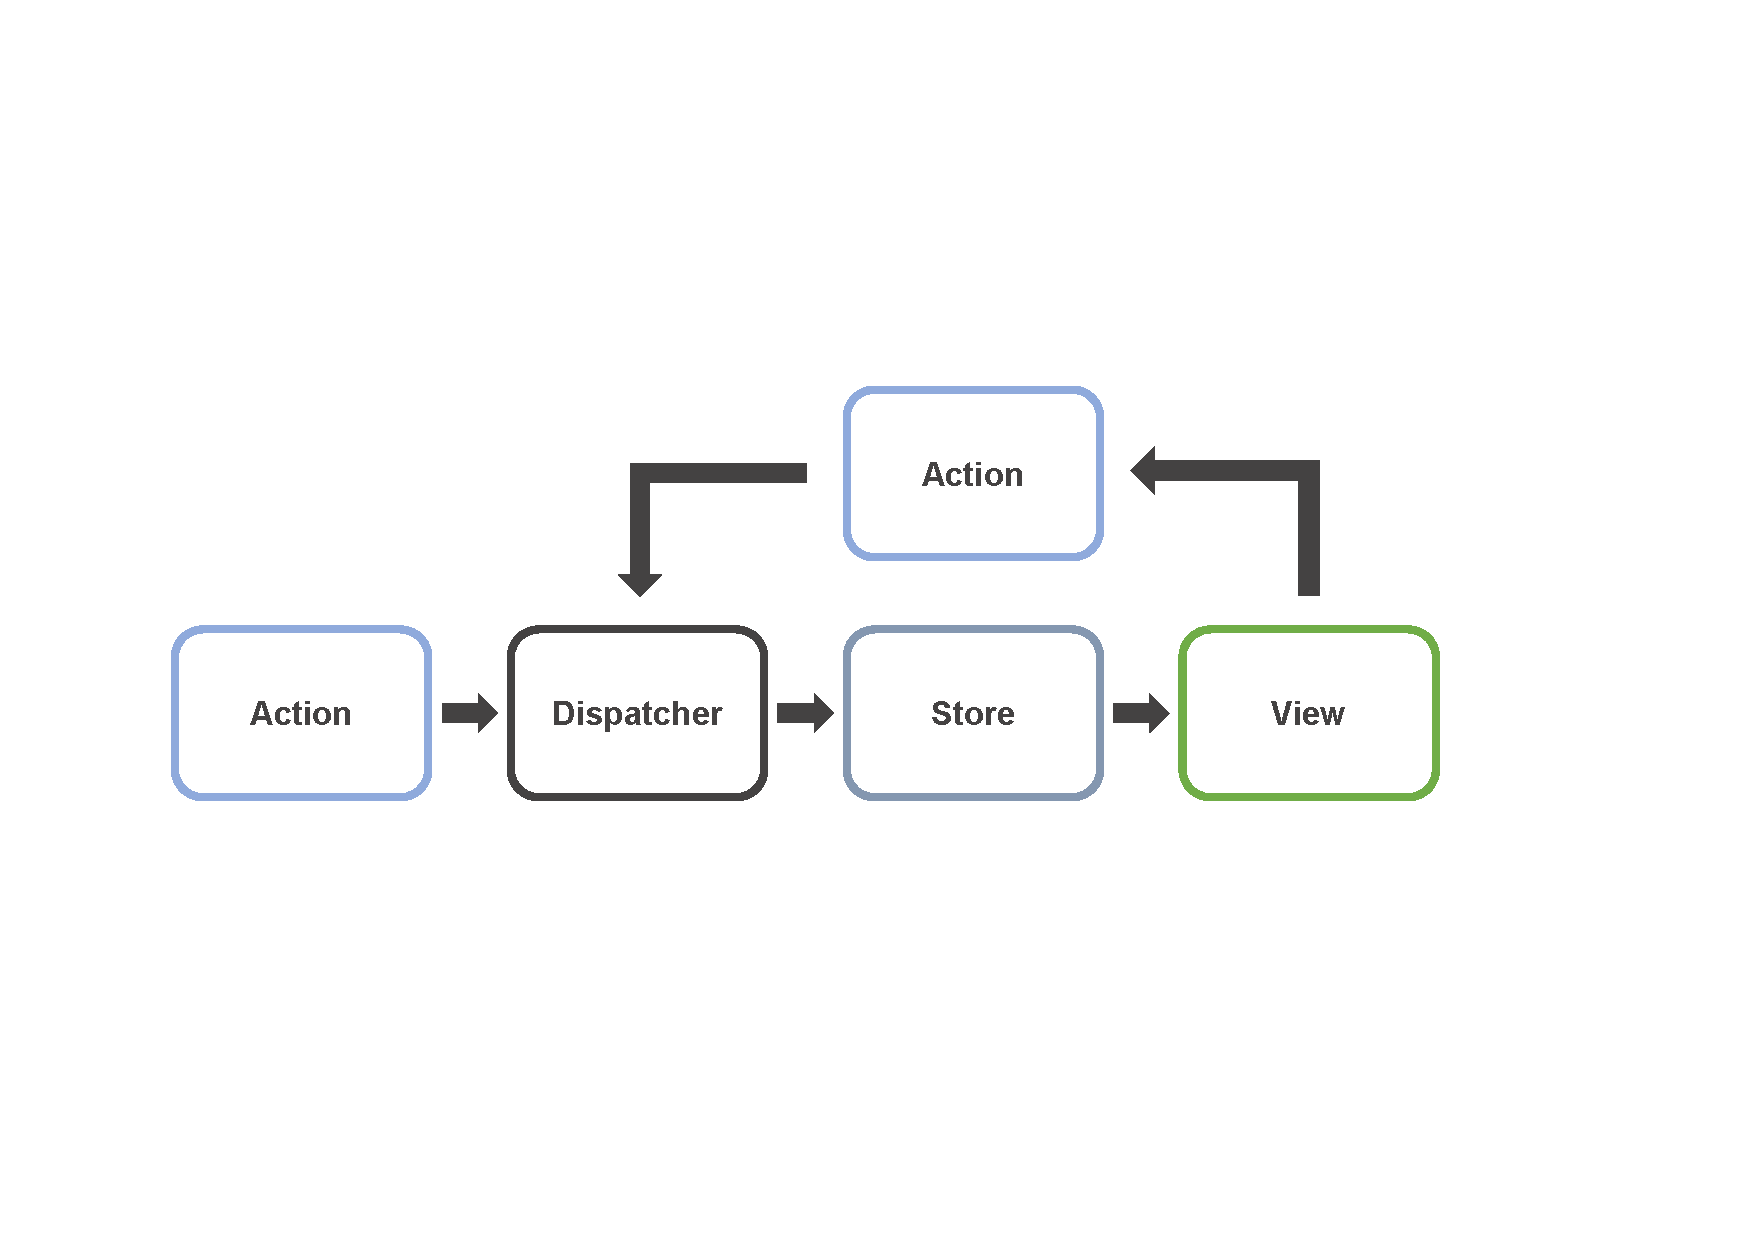
\includegraphics[scale=.6, trim= 2.5cm 6cm 4cm 6cm, clip]{002Flux.pdf}
  \caption{Flux application architecture \cite[as in][structure-and-data-flow]{FacebookInc.2014}}
  \label{fig:FluxArchitecture}
\end{figure}

After understanding the fundamental concept of Flux, it should also be of interest for the programmer to fully understand the function of each component of the paradigm. It is important to know about the whole concept and all of its components to further being able to understand implementations of Flux or Flux frameworks.

\subsection{Dispatcher}

In the documentation \cite[a-single-dispatcher]{FacebookInc.2014}, a Dispatcher is specified as a "central hub that manages all dataflow in a Flux application". A very important fact stated in \cite[actions]{FacebookInc.2014} is, that a Dispatcher exposes a method, which can be passed an Action. If provided an Action via that method, the Dispatcher then dispatches that Action to all Stores, triggering an update only on Stores that can react to the dispatched Action. One of the biggest advantages is that many Stores can react to the same Action, which makes the application highly scalable and extensible.  

The dispatcher can also explicitly handle more than one Store by handling their registered callbacks in a specified order, if that behavior is desired by the web application programmer.

When the application grows, there can be more than one Action set. The programmer should logically divide all available actions into different files to keep the application organized. This does not change the fact that all actions are dispatched with the same Dispatcher to all registered Stores. 

\subsection{Store}
\label{ssec:fluxstore}

% revisit citations

As it can be read in \cite[structure-and-data-flow, Stores]{FacebookInc.2014}, a Store contains an application-specific state and data, as well as data manipulation logic. Every Store has to be registered to the Dispatcher by registering a callback. 

Registered callbacks can be used to handle asynchronous data change events in the Store. The Dispatcher uses the Store's callbacks to determine when a data transaction or manipulation has finished in order to being able to dispatch a new action. Registered callbacks are also used to dispatch actions in a specific order to more than one Store.

As mentioned above, Stores also contain data manipulation logic. The way Stores work in conjunction with Dispatchers is that the Dispatcher dispatches one Action to all registered Stores. Each Store can react to that dispatched Action with its own internal data reducing functions.

\subsection{View}

The View component is responsible for correctly displaying any state of provided data as described in \cite[views-and-controller-views]{FacebookInc.2014}. To achieve that, so called Controller-Views can handle data from any Store and also pass it down to any nested component in the view hierarchy.

Controller-Views react to Store update events and can update whole child component trees by updating their own internal state. By reacting to any data changing event, the Controller-View triggers an update for its child component tree. Each child component can then process the passed data from the parent component, only processing component relevant data. The programmer could even decide to pass a whole Store's data to a Controller-View.

Every important section of a web application should be considered as a Controller-View. In ReactJS it is very easy to determine what components are Controller-Views. As explained in Chapter \ref{cha:ReactJS}, ReactJS Containers are the so called \enquote{smart} components and could be considered as Controller-Views in the Flux pattern. Again, the Flux pattern works exceptionally well with ReactJS, as ReactJS components automatically trigger a render refresh if component properties change. With Flux the programmer only has to introduce a root component bound to the Stores data in order to automatically re-render the application if the Store's data has changed.

\subsection{Action} \label{ssec:fluxaction}

The creation of Actions is handled by action creator methods worked out in \cite[structure-and-data-flow, actions]{FacebookInc.2014}. An Action can be created by a user interaction through an event handler of the corresponding view, through an initialization of a component or even through the server sending an error code for example. As explained before, the Action is then dispatched to the Stores to be handled and to manipulate the Stores to the desired state.

If the application needs to communicate with some kind of API or execute any asynchronous operation it is usually handled inside the action-creator methods. These asynchronous operations are performed and data that might result from those API-calls is then bundled into the Action and dispatched via the Dispatcher.

\section{Overview of MVC}

%% history explanation
%% fowler sehr interessant mit view und controller observed model
%% problem -> javascript nicht interchangable components, keine interfaces, patterns? flux hoax? omg :O

As mentioned before, MVC is the most common application architecture in the web. To understand the differences between Flux and MVC, this section provides all necessary information about MVC. That information is intended to help the reader to understand the arguments of the comparison between the two paradigms in this bachelor's thesis. This paper, however, assumes that the reader has a basic understanding of the MVC architecture. Due to that assumption, the overview of each aspect of the MVC pattern is rather short and only shows how this paper is referring to each component of the architecture.

\begin{figure}
  \centering
  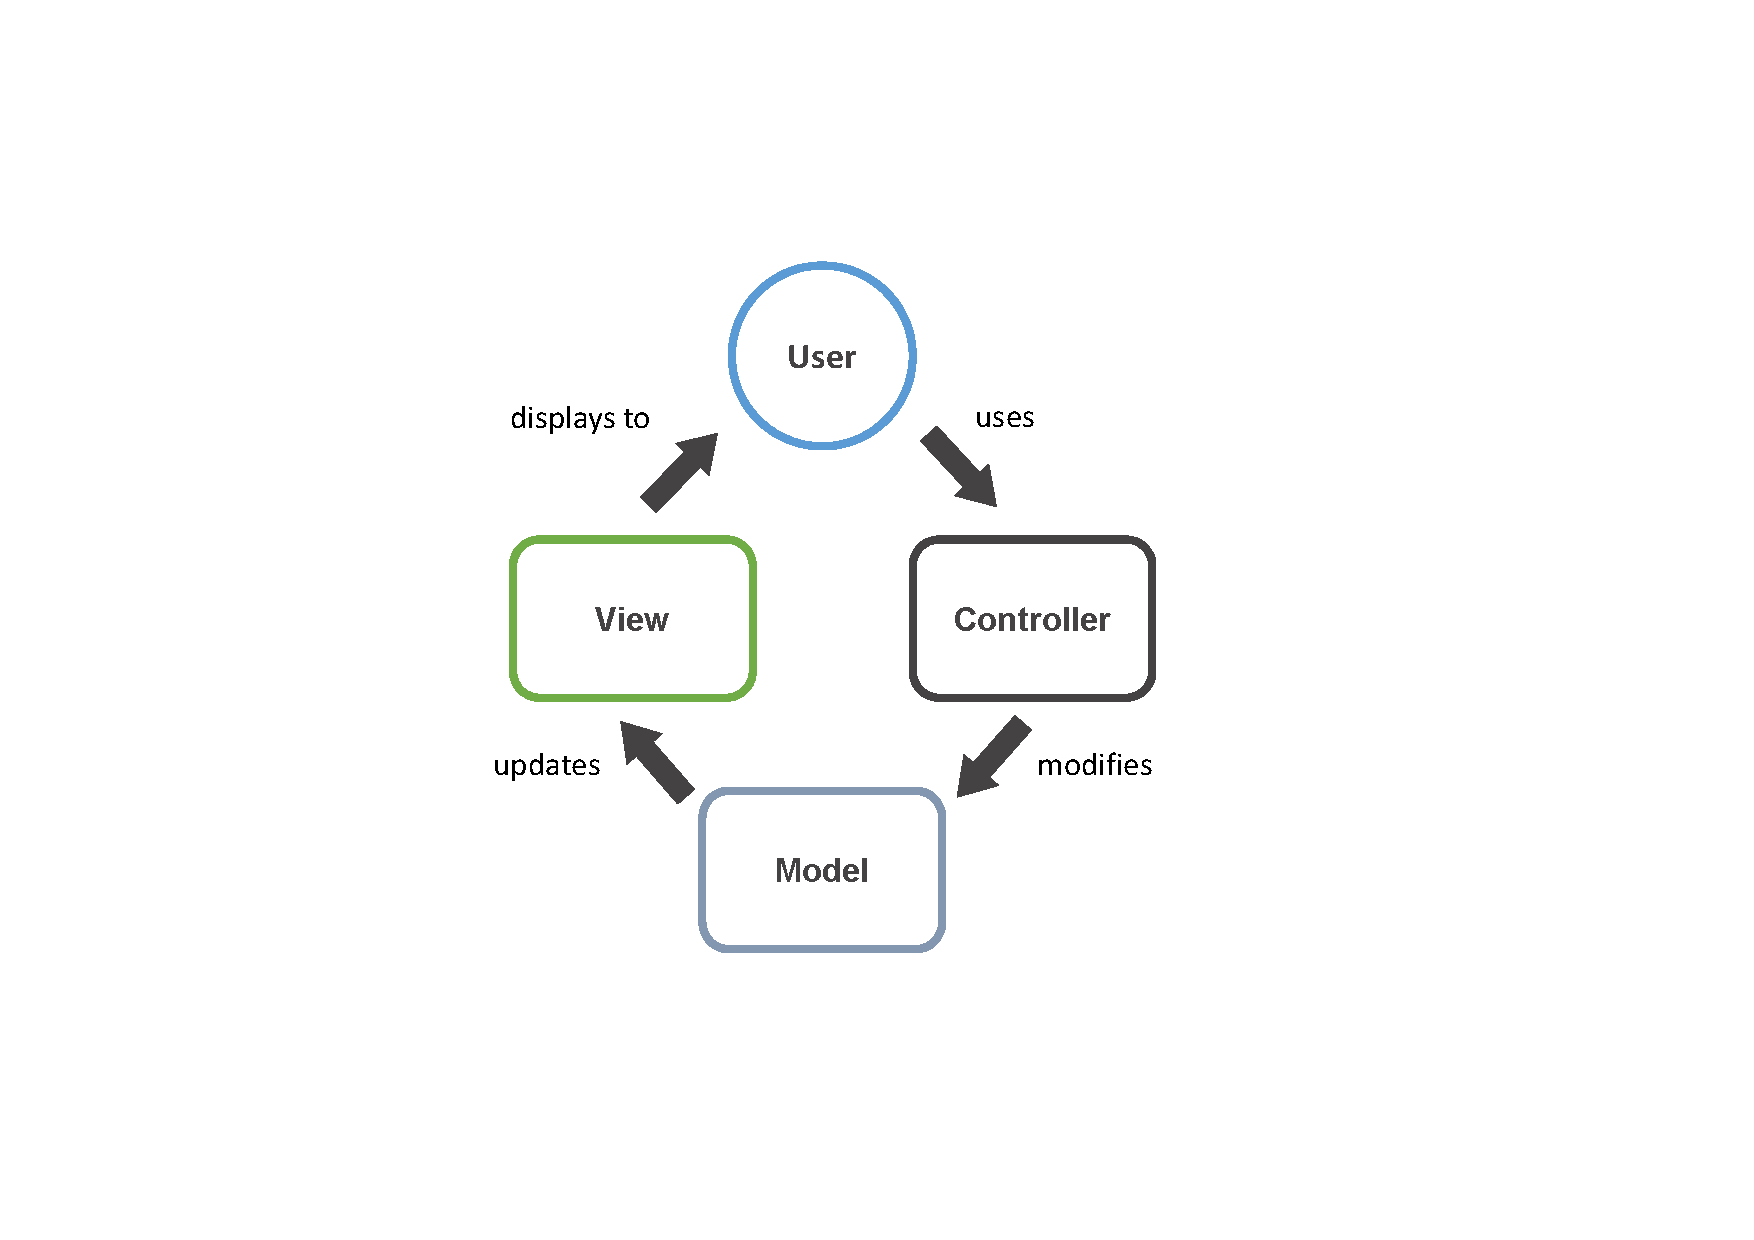
\includegraphics[scale=.7, trim= 4cm 4cm 4cm 4cm, clip]{005tradfrontendmvc.pdf}
  \caption{traditional MVC \cite[interpreted from][1.3 Traditional MVC]{stefanoborini.2014}}
  \label{fig:tradmvc}
\end{figure}

\subsection{Introduction and history}

Traditional MVC as it was initially invented and intended actually also lets data flow in one direction as shown in the Figure \ref{fig:tradmvc}. The programming pattern was invented around the year 1970 to 1980 when the concept of a user interface was not very common \cite[\#ModelViewController]{MartinFowler.2006}. The main goal was to make code of user interface applications reusable and to find a way to make UI applications scalable.

The new MVC pattern was also invented to avoid the so called "Smart-UI" anti-pattern \cite[S.11,S.13]{MattiBragge.2013}. In that paradigm there is no separation of concerns meaning that every part of the application logic is located in the interface code. It should be clear for every programmer though that such conditions should be avoided to keep the application scalable and to keep every component of the application interchangeable.

% revisit this sentence

The fact that many people are using the MVC pattern in their applications is also the reason why the pattern has many variations. There are also many different ways on how it is possible to implement an application using the programming paradigm. There are many interpretations of various aspects of the application architecture that can lead to a false understanding of MVC. This chapter will cover some of the possible misinterpretations of MVC and show how the pattern has evolved over time. It is very important get an overview to the MVC pattern in order to being able to compare it to other competing application architectures.

\begin{figure}
  \centering
  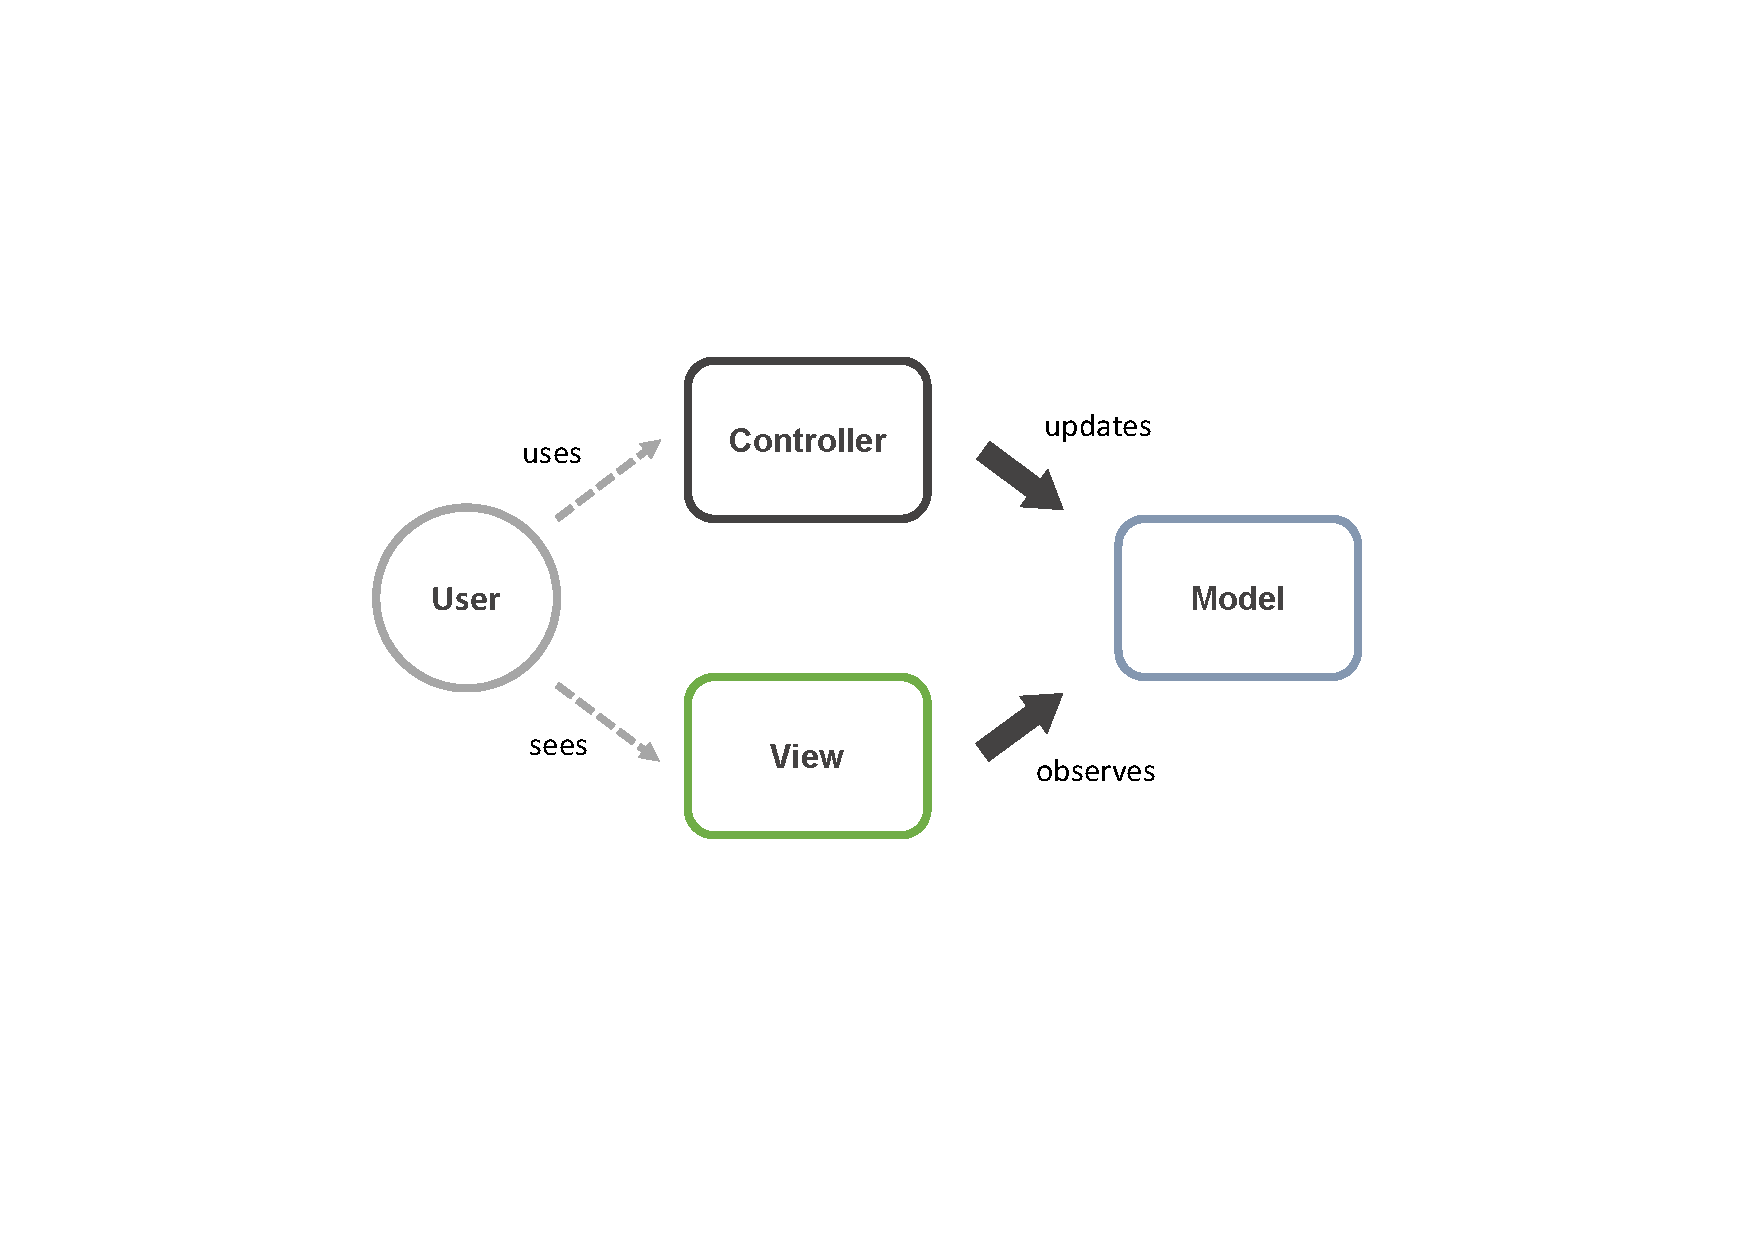
\includegraphics[scale=.7, trim= 4cm 5cm 2cm 5cm, clip]{006fowlermvc.pdf}
  \caption{another interpretation of MVC \cite[seen by][\#ModelViewController]{MartinFowler.2006}}
  \label{fig:fowlermvc}
\end{figure}

\subsection{Model}

In this paper the term "Model" is not used to represent the business logic part of the application but rather the representation of the actual application state or "real data" that is used to represent a certain state of the View (Presentation-Model). But what exactly is the Model then? In \cite[1.4.1 Model]{stefanoborini.2014} the Model is described as the component that either contains stored data or functionality to compute view-relevant data. 

The Figure \ref{fig:tradmvc} shows that the model is responsible for updating the View. Every change in the state of the model will trigger an update in the View component but not the other way around. 

According to Martin Fowler, in the Figure \ref{fig:fowlermvc}, the Model is the passive component. Fowler's MVC diagram (\ref{fig:fowlermvc}) shows the interaction arrow between Model and View in the opposite direction than the traditional MVC diagram (\ref{fig:tradmvc}). Nevertheless, this does not imply that data is flowing in the different direction---quite the opposite---the Model is still storing the data and the View observes the Model. The View is only updated when the state of the Model changes. As described in \cite[\#ModelViewController]{MartinFowler.2006} the Model is completely ignorant of the View component and only Stores data that is used to represent the visual state of an application.

\subsection{View}

% revisit citation

The most important part, that can't be stressed enough, is described in \cite[1.4.2 View]{stefanoborini.2014}. The View is the component that handles interaction of the user but in \textbf{read-only} mode. This implies that the component is incapable of modifying the state of the application. A View should therefore only contain logic that exactly tells the component what to represent or display at a certain state. When following the MVC pattern a View component must not call any API endpoints, nor query any database. According to \cite[1.4.2 View]{stefanoborini.2014} the View observes the Model to know when to update and what to display to the user. 

Figures \ref{fig:tradmvc} and \ref{fig:fowlermvc} show the relation between the View and the Model differently but the flow of the data is the same. Data always comes from the Model and is transferred into the View. How data is transferred is dependent on the actual implementation. In most cases the View observes the Model, updates itself if the Model changes, and is then seen by the user. 

\subsection{Controller}

As mentioned before, the View aspect of the programming pattern MVC enables the user to interact with the application. When there is a user interaction though, the View should delegate this action to the so called Controller that can then react to that user input and handle it accordingly as described in \cite[S.14]{MattiBragge.2013}. \cite[1.4.3. Controller]{stefanoborini.2014} describes the Controller as a component that interacts with the Model in read-write mode. It is the business logic of the View, so to speak. 

Furthermore, there is always a Controller-View pair for every part of the application that has its own visual representation (\cite[\#ModelViewController]{MartinFowler.2006}). An example would be an application that has a login screen and one or more screens to interact with provided services. The application would at least have to have 2 or more View-Controller pairs.

The MVC pattern is often referred as triad but it is important to not forget about the most important part about MVC, the user. Figures \ref{fig:tradmvc} and \ref{fig:fowlermvc} show, the user is added to the triad to improve the visualization of data-flow of the application.

\subsection{Traditional or client-side MVC versus server-side MVC}

% it is getting interesting now :O cite him -> \cite{PaulCowan.2013} -> server / clientside mvc 
% also cite him \cite{ChristianAlfoni.2015}
% another really important point to make is...
% here i will compare traditional mvc to serverside mvc. when ppl talk about mvc they usually refer to forms of serverside mvc through php and so on, this is wrong, explain problematic of that and show what real mvc is... 

Because the development of MVC started in the 1970s, the software pattern has changed and evolved much until now. It is very important to clearly understand the difference between the aspects of the programming paradigm as MVC in some cases does not equal MVC. In this paper, the most important distinction to know about is traditional and the server-side variant of the software pattern.

When reading this section, it is important to point out that this paper refers to "traditional MVC" as is was developed in the 1970s by the smalltalk community. The article \cite{ChristianAlfoni.2015}, on the other hand, uses the term "traditional MVC" for the version of MVC many people nowadays refer to, the server-side variant of MVC. Another term for "traditional MVC" could be "client-side MVC" as this makes clear that the state only exists on the client.

Traditional MVC was initially developed for applications that keep state and data on the same machine. Nowadays, applications are split into more layers. Modern software is usually deployed at least on an application and a database server. Especially in the web, applications additionally have to be served over the HTTP-protocol adding yet another layer.
 
The article \cite{ChristianAlfoni.2015} states that the biggest problem with server-side MVC is the fact, that the View cannot observe the Model as it was initially designed by the smalltalk community in the 1970s. The fact, that there is a HTTP layer between the View and the Model (visualized in the Figure \ref{fig:serversidemvc}) makes it impossible for the View to automatically update when the application state is changed. It always has to be the View initializing the update process. The problem is, that HTTP is a stateless protocol constraining the View to only being able to change the application state during one HTTP-request (\cite{PaulCowan.2013}). This also implies, that the only component that can persist state is the View due to the stateless protocol violating the original concept of MVC.

In the web many frameworks that are written in PHP for example heavily rely on the server-side version of MVC because they send fully generated and fully rendered views to the client and handle all logic on the server. In that case, it is the Controller that is responsible for sending the View to the client (Figure \ref{fig:serversidemvc}). In the last years, so called "single-paged applications" became popular among the web community. These single-paged applications are downloaded and executed only on the client. This makes it possible to use traditional or client-side MVC again as there can be application state, that is able to persist during the whole execution time of the software.

\begin{figure}
  \centering
  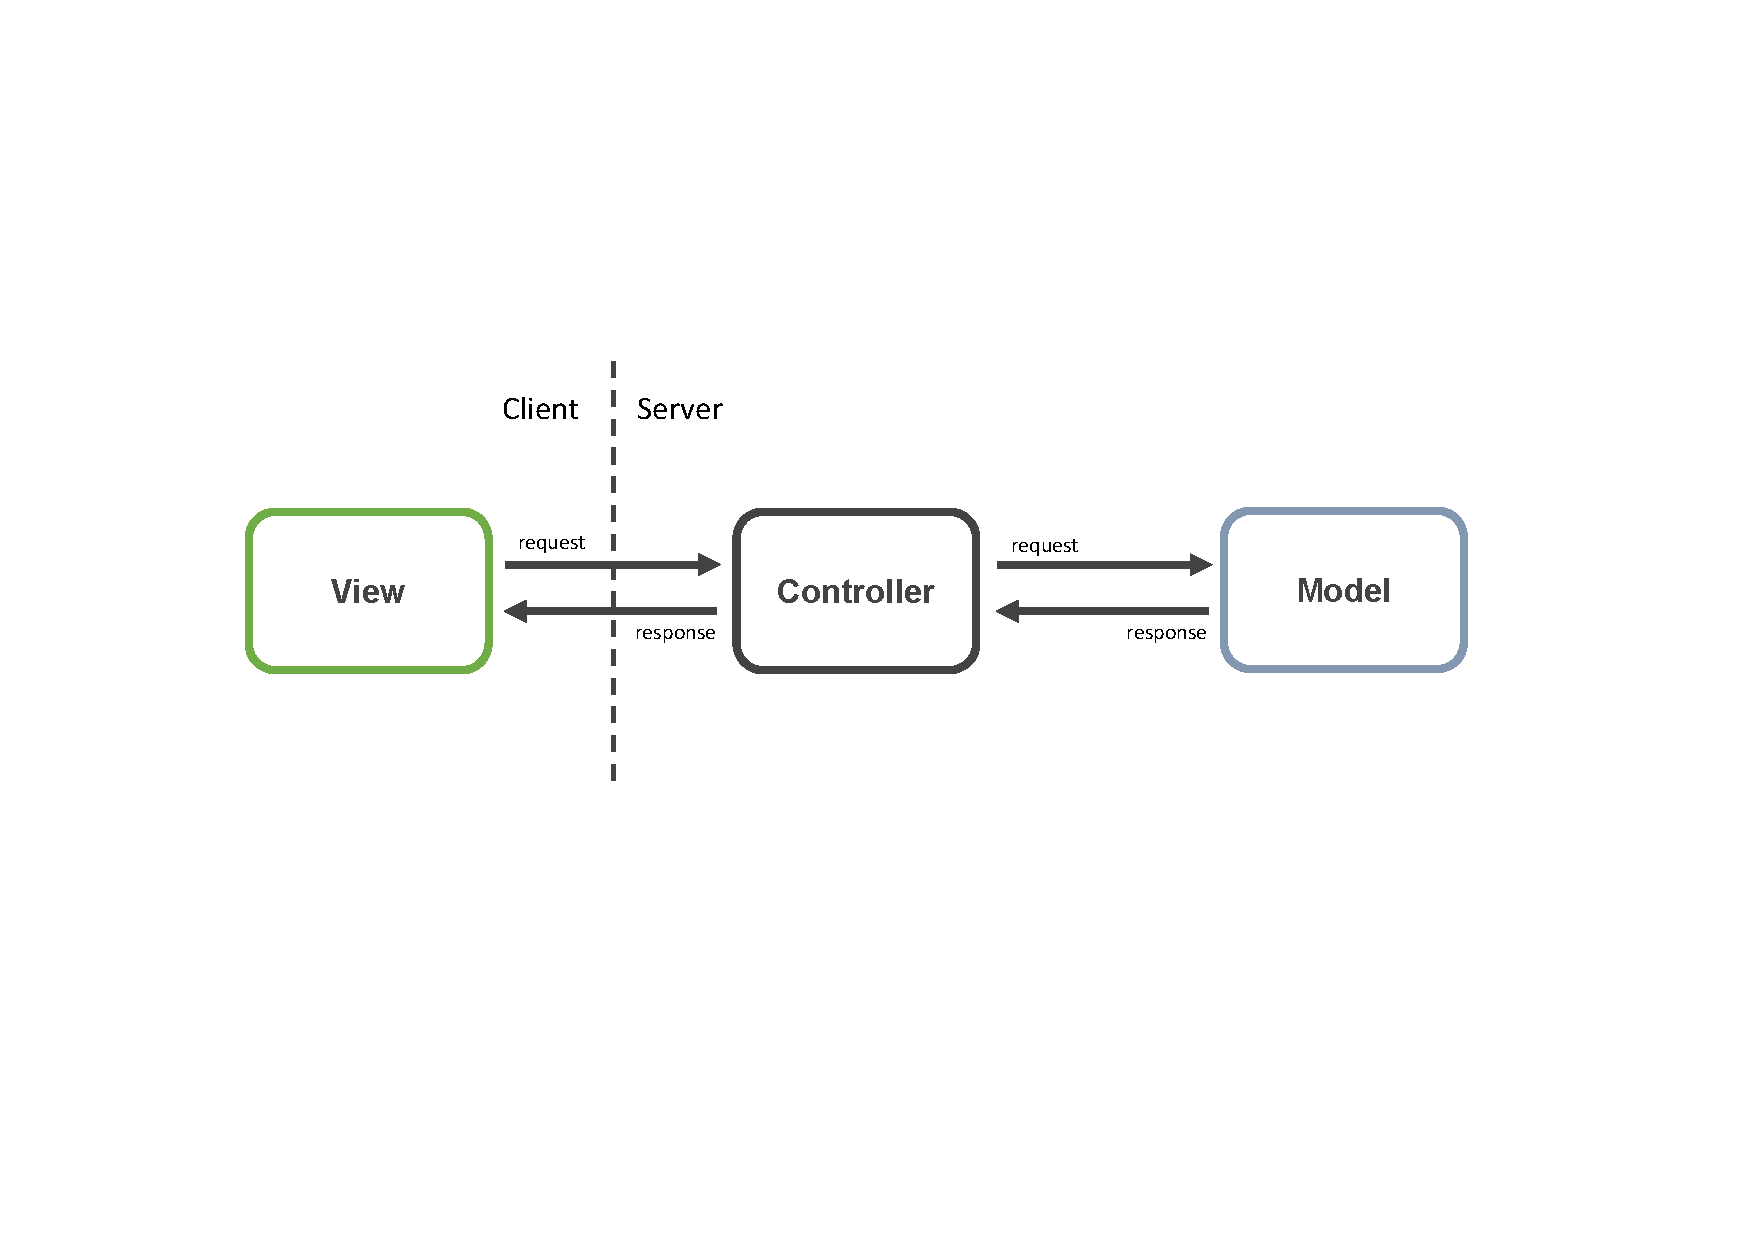
\includegraphics[scale=.7, trim= 4cm 7cm 3cm 5cm, clip]{004serversidemvc.pdf}
  \caption{MVC in a server-client environment \cite[as in][]{ChristianAlfoni.2015}}
  \label{fig:serversidemvc}
\end{figure}

\section{Comparison of the software patterns}

In this section, the Flux and the MVC pattern will be compared. Now that the reader has a basic understanding of what the Flux pattern is about and what it will be compared to it is easier to develop an opinion based on the provided facts. When new software patterns are introduced, it is essential to carefully and critically compare them to existing ones and evaluate their usefulness in the modern software environment, where they can possibly be used.

\subsection{General facts and misconceptions}

% write about data only being updated over the controller is sometimes a big overhead
% maybe include wrong graphs?
% react does not really have a model itself

When casually searching the Internet for the Model View Controller pattern, many visual representations of the software architecture can be found. In many cases the diagrams show the MVC-triad with arrows in facing different directions, unidirectional and bidirectional, leading to confusion and raising the question in what direction data flows exactly. 

Diagrams that show the Model update the View and the View in return update the Model stimulated by user input are quite simply wrong. This is a common misconception. Change of the application state should only be triggered over the Controller. Everything else would imply a violation of the MVC pattern.

In this bachelor's thesis there are two representations of MVC (\ref{fig:tradmvc} and \ref{fig:fowlermvc}). Both representations show the same components but different relations. It must be understood though, that data-flow still goes in one direction. Different names for relations may switch the directions of some arrows in a diagram but do not change the semantic meaning of the MVC pattern.

In the presentation where Facebook introduces the supposedly new software architecture Flux (\cite{youtube.2014}), the speaker presents the audience a visualization of MVC that can be seen in the Figure \ref{fig:mvcalafacebook}. Facebook talks about how complicated the debugging process was because of countless bidirectional relations between the View and the Model components. To the attentive reader it should be clear, that a bidirectional relation between the View and Model component regarding to data-flow implies a violation of the MVC pattern. The question arises if Facebook's engineers had understood the programming paradigm MVC before developing an allegedly new programming paradigm?

% way react works view easily can update model

\begin{figure}
  \centering
  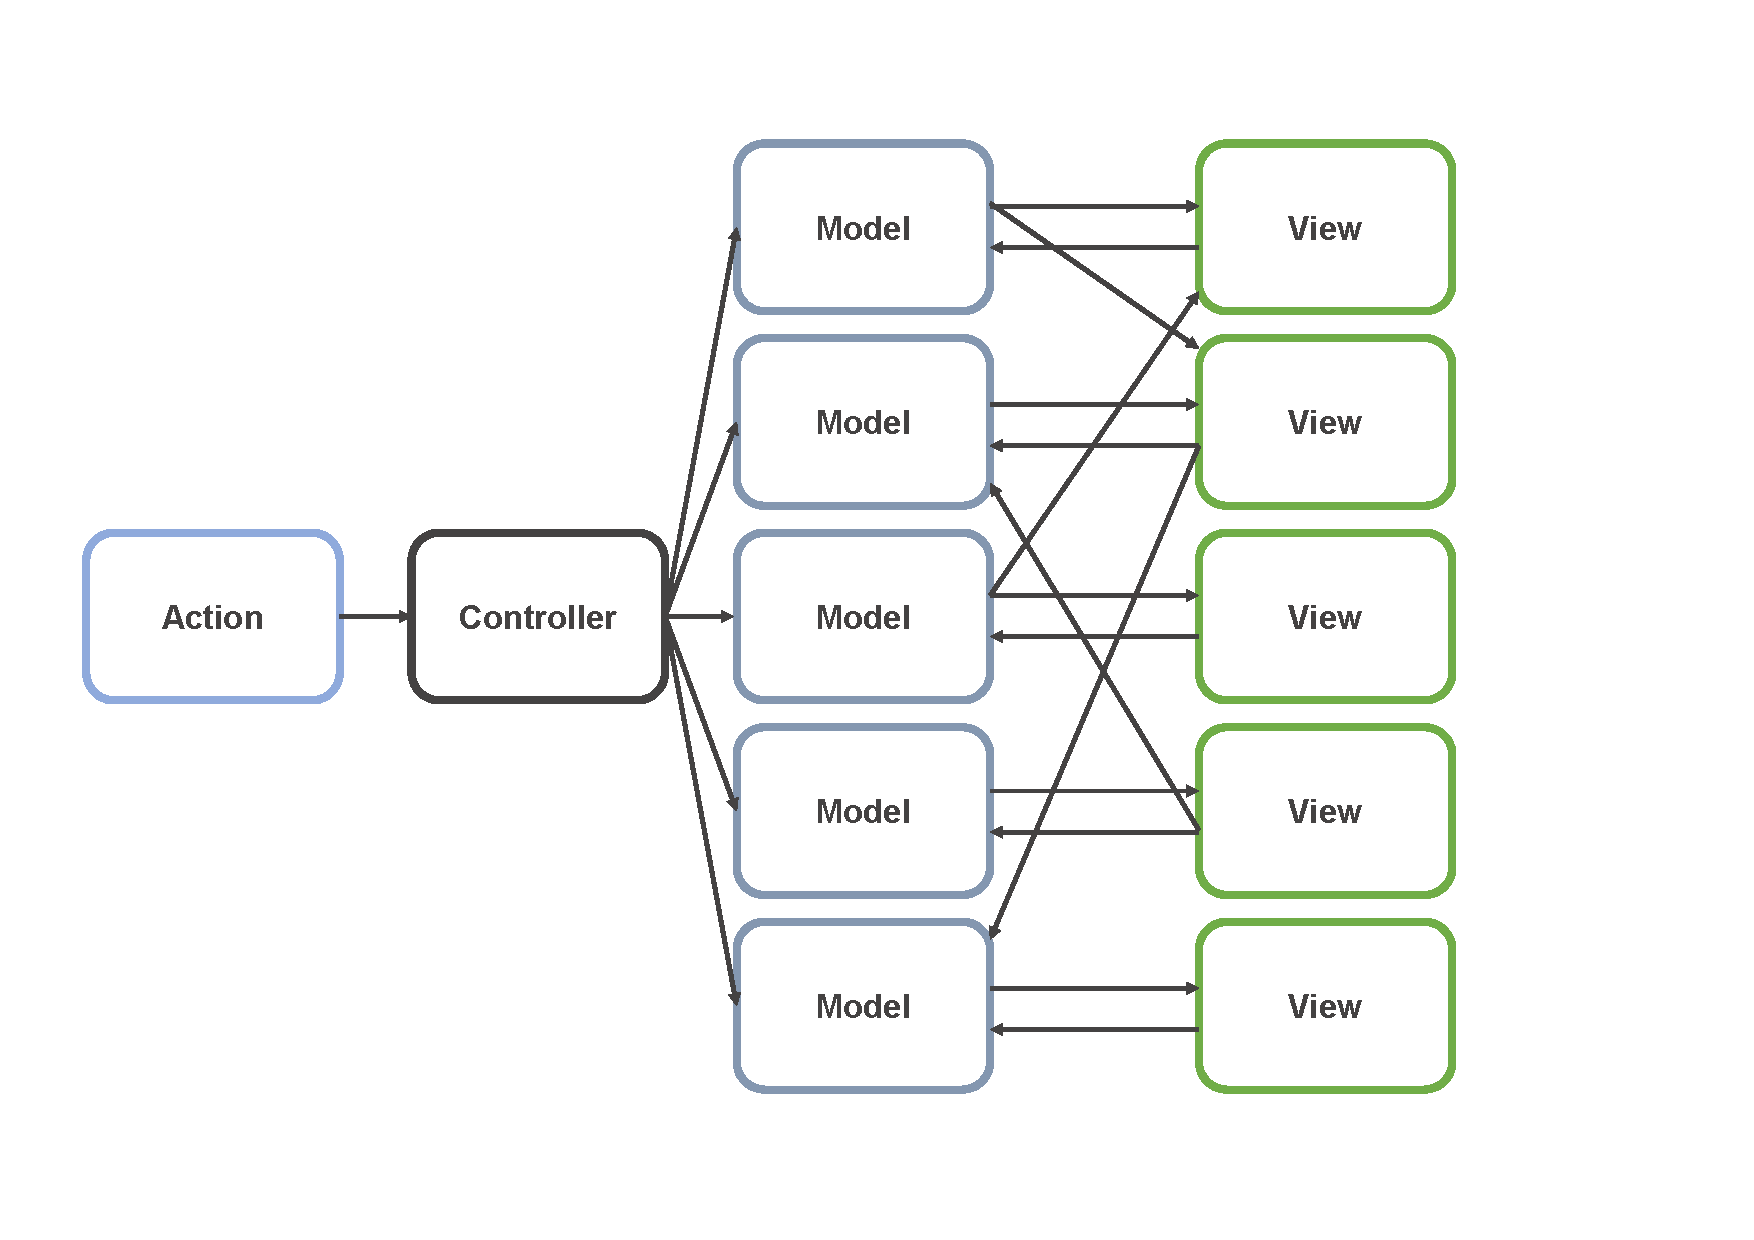
\includegraphics[scale=.6, trim= 1cm 2cm 0 2cm, clip]{003MVCalafacebook.pdf}
  \caption{MVC as Facebook describes it in \cite[11:10]{youtube.2014}}
  \label{fig:mvcalafacebook}
\end{figure}

\subsection{Similarities of Flux and MVC}

Looking at the illustrations of Flux (\ref{fig:FluxArchitecture}) and MVC (\ref{fig:tradmvc}) it can be observed that there are similarities. Flux achieves its unidirectional data-flow by only changing the Store's data by dispatching an Action containing relevant user input data over the Dispatcher. Comparing this behavior to the MVC application architecture, it should be clear that the operation of a change in the Model triggered by a user stimulus handled by the Controller is a quite similar behavior.

One of Flux's biggest advantages, according to Facebook, is the possibility of having global Stores. These global Stores can be used for an application state which has to be used in many different parts of the application e.g. a notification counter that shows the user a count of unread messages. Traditional MVC according to Fowler (\cite[\#ModelViewContoller]{MartinFowler.2006}) needs to have a Controller-View pair for every screen in the user interface but also one global Model that stores the application's state. In most cases though, it is recommended to also divide the Models into the logic sections of the application to make the code more transparent and easier to read and debug. This is very similar to how Flux handles global data. Like in Flux in MVC it is also allowed for more Views to observe the same model.

The MVC triad consists of three components: the View, the Model, and the Controller (\ref{fig:tradmvc}, \ref{fig:fowlermvc}). One could add the User as the fourth optional component that makes the architecture easier to understand. It is the user's stimulus that triggers every action or state change in the application. When looking at the Flux pattern (Figure \ref{fig:FluxArchitecture}) there are also three components that have the same function as the corresponding components in the MVC diagram. Flux's Dispatcher, for instance, could be seen as MVC's controller and the Store is similar if not identical to MVC's Model.

% compare mvc to flux and see the similarities. even tough the patterns are similar it is a good pattern though. Real advantage is immutability though, talk about this later maybe?
% store is global, mvc has no best practice... maybe singleton

\subsection{Differences of Flux and MVC}

One of the biggest differences between Flux and MVC is the way the View component reacts to a change in the application state. In the Flux pattern the View is updated by injecting the new application state into the View. The View component is a strict representation of what has to be displayed at a certain state. Updates therefore happen implicitly. MVC on the other hand handles updates in the application state by binding the View to certain values and thus observing the Model. When a Controller modifies the Model every View that has bound its view-components on data in the Model can automatically update. The MVC View updates itself automatically whereas Flux's View component is updated by the new state that is injected into it.

Another big difference is the way application state is modified. As mentioned before, Flux uses a system where Actions that contain data are dispatched to the Stores which then accordingly react to the dispatched Action and update their data via reducing functions. MVC on the other hand should not have any logic in its Model. Because the Model should only be a representation of Data the Controller must handle API-calls and directly access the Model to change its data.

% state that flux implicitely updates the view and mvc uses an observer pattern
% stores selectively react to action? MVC?

\subsection{Advantages and Disadvantages of Flux and MVC}

A few years ago web developers could not think about another way to engineer a web application other than sending a fully rendered application View to the client and handling user input logic and state on the server. Programmers therefore can only update the View by triggering a change in the state by executing logic in the corresponding Controller. The biggest problem with this approach is that it violates the constraints of traditional MVC as it was designed initially. The Controller and Model instances only live during an HTTP-request, making it impossible to follow MVC's constraint of persisting a Model state during the lifetime of the application. Another big disadvantage is the fact that the View cannot be automatically updated, nor can it observe the model state because of the additional stateless HTTP-layer.

A disadvantage of both patterns is of course programming overhead. Applying a highly complicated application architecture to software always implies increased programming time. What really matters are the long term advantages tough. By using either the Flux or the MVC pattern when developing web applications it makes components interchangeable and increases the application's scalability. Even web applications written in JavaScript for example can heavily benefit from using either one of the mentioned programming paradigms.

% application model domain model difference -> bragge 19
% serverside cant use persisting global state

\section{Conclusion}

Even though the Flux application architecture seems to be extremely similar to traditional MVC, Flux is still an excellent choice for a web application architecture. On its own, MVC has proven itself over the course of the time of its existence. There has been a big shift in how web applications are build until now. Nowadays, many big web applications are built as single-paged applications and the number is steadily growing. The biggest advantage of having an autonomous application that is executed only on the client opens up the possibility to keep application state on the client without having to reload the web page every single time when the application state changes.

The use of single-page applications do not only enable Flux application architecture to be used, the MVC programming pattern can be applied as well of course. Other frameworks like AngularJS for instance use a special variation of MVC called Model-View-ViewModel (MVVM). It is safe to say that using a programming paradigm like Flux or MVC is of utter importance nowadays when building web applications. Not only does it add structure to the code base, but it also makes code much more readable and easier to understand for developers who have not implemented the application but later have to maintain it.

Initially Facebook presented Flux as a big way forward but upon further review it appears as if Flux was just another variation of MVC. There are many similarities that make the two patterns seem to be very alike. It is honestly disappointing to discover that a much praised and hyped application architecture proposal, which had promised many improvements on how to improve web application development, is just a shallow copy of a present paradigm (MVC) that has existed for many years until now. 

It must be emphasized though that Flux is not a bad application architecture approach at all. All the similarities to MVC make Flux a solid pattern that has its merits on its own. After much research it is clear that both patterns can yield enormous advantages if they are used to design web applications. Having no application architecture at all is of course the worst decision a programmer could make. Also, MVC and Flux seem to be very popular among the web developer community.

Upon further reflection it seems as if Facebook did not research properly and implemented MVC wrong. That was the reason why the company came up with a proposal of an allegedly new paradigm. Proof for this theory is the diagram (Figure \ref{fig:mvcalafacebook}) in the video presentation \cite{youtube.2014} which clearly shows that the gist of the MVC paradigm was not understood correctly. 

After having used Flux as a paradigm for a web application it is clear that the architecture seems to be tailored for one specific framework which is ReactJS. The next chapter will show exactly how Flux perfectly fits into the mindset of ReactJS and how it works really well with the framework making it a very satisfying experience to build an application with a good architecture and seeing the benefits of using such a paradigm.

In conclusion it is very important for web application development to use some form of sophisticated application architecture. The number of applications that rely on some form of web technology is increasing heavily nowadays and thus it is even more important to emphasize the necessity to use a well thought through application architecture.

% initially facebook presented flux as a big way forward
% flux was presented ad
% upon review, after research was completed
% after a closer inspection
% after considering the findings / data
% it is clear -> instead of i believe -> flux has only minor advantages / it is only marginally different
% the advantages to not outweigh / the advantages are negligent in comparison
% after review it was conluded / found --> take it for I
% conclusion facebook lied -> make point upon further reflectoin i came to realize flux not that advantageous as i initially thought

\chapter{ReactJS}
\label{cha:ReactJS}

% one of biggest advantages is component based
% functional programming

In the previous chapter the application architecture Flux was introduced and discussed. Even tough aspects of this programming paradigm seem to be copied from other programming patterns, it is certain that Flux is not a bad application architecture after all. This section will demonstrate how Flux works best with Facebook's front end framework ReactJS (\cite{FacebookInc.2013}). The goal is to show the reader what is necessary to develop a web application by using cutting edge web technologies. This chapter will also provide an overview over some best practices and help the user to make application architectural decisions.

A few questions will come to mind: \enquote{What tools are needed to develop a \mbox{ReactJS} application?} or \enquote{Why should a web application programmer use this framework?}. Nowadays many large companies use JavaScript frameworks for the development of their web applications. The hard part in starting any web application project is to decide, which framework or technology is will be used. After reading this chapter all mentioned questions will be answered and it should be easier to make the right decision. This paper is \emph{not} a comparison between competing web technologies but it should give a clear overview of the features and benefits when using ReactJS.

\section{Why ReactJS?} \label{sec:whyreactjs}

As described in \cite[S.7-8]{Zeigermann.2016} there are several reasons why ReactJS is a good choice for a JavaScript front end Framework as described in the following paragraphs:

First of all, the framework is rather easy to learn and understand to get going and to simply start coding. There are some easy code examples \cite[Docs: Hello World]{FacebookInc.2013} to get started very easily. The difficulty is not very high even for programmers that do not have much experience at all. There is also always a link to a live coding website where basic ReactJS code examples can be tried out.

React's API is not extensive and well documented. The architectural decisions of the framework and the code of an application make it more easy to understand. Furthermore the ReactJS API hardly ever alters in a way that breaks already existing code. Facebook claims on many articles in their blog \cite[Blog]{FacebookInc.2013} that almost no time is wasted in refactoring deprecated ReactJS code from any outdated application. Experience has shown that indeed there had not been any situation where any front end specific code of ReactJS broke by updating to a newer version of ReactJS. If some component is about to be deprecated, it is clearly communicated on the release notes on the blog or by runtime development deprecation warnings that link to migration guides. 

ReactJS is a view-only framework. As stated on the project's starting page \cite{FacebookInc.2013}, Facebook does not make any assumptions about the development stack of the programmer. It is completely up to the software engineer to choose what technologies to use in conjunction with ReactJS. There are very few requirements from the framework itself. For instance it is totally up to the developer how to handle routing, application state and the communication to an API. That is also the reason why this framework appears to be very professional, as it is the programmer's responsibility to develop an application architecture and to choose the suiting development tools to tailor the application to the client's needs.

The ReactJS framework exists since the year 2013. During the time of its existence many technologies have been developed that work really well with this framework. Being highly component oriented it is possible to easily integrate third party ReactJS components from other developers. Custom ReactJS components are open source most of the time and can be integrated into any ReactJS project by using some form of a package manager. For example there are high-performance list or table views with lazy loading that optimize handling large amounts of data. Integrating those components can save a lot of time and improve the application's performance without the developer having to implement complicated components by him- or herself. 

Another advantage in developing ReactJS applications is that this framework has been in use long enough so there are many excellent developing tools available at the programmer's disposal. Everything from performance benchmarking tools to ReactJS component explorers can be integrated in any \mbox{ReactJS} project. One of the most important pieces of developing tools would be the possibility to automatically recompile and reload the application when files change without loosing the application state.

ReactJS is often compared to other frameworks in terms of performance and scalability. There is no definite answer which framework is the best amongst them of course. The fact that not only Facebook itself uses the framework but also other well known large well known companies like AirBnB\footnote{https://www.airbnb.com} or Plex\footnote{https://plex.tv/} as well provides good evidence that the framework can be well performing and scalable if implemented correctly.

% It should be mentioned that ReactJS is not only used by Facebook. Other well known large companies like AirBnB or Plex use the library as well. This is good evidence that the framework can be highly performant and scaleable if implemented correctly. 

\section{Introduction to the tooling for ReactJS}

When developing a \mbox{ReactJS} application, it is of utmost importance to understand all the tooling that is necessary to develop a ReactJS application. The technology which is necessary to transform \mbox{JavaScript} code into a code bundle that can be interpreted by the browser should not be a \enquote{black box} to the developer. When talking about a \mbox{ReactJS} application it often implies that the term \enquote{single paged application} is clear to the programmer as well. This section will explain all those terms and all necessary tools to create such a single paged application by using ReactJS.

%%here it should be stated why any sane person would go through the process of insane JavaScript npm or webpack processes to develop a web application.

\subsection{ECMAScript and Babel}

%here i will explain how to use stage-0 features of the JavaScript language that don't even have an implementation yet and why one would want to use these features.

\mbox{ECMAScript}\footnote{https://www.ecma-international.org} or ES for short is a specification for scripting languages and also specifies the scripting language \mbox{JavaScript}. \mbox{ECMAScript} is developed by \mbox{ECMA International}. Because \mbox{JavaScript} is a scripting language it needs to be interpreted by a JavaScript engine. The problem is, that ECMAScript is only a specification and different engines implement different versions of ECMAScript. Oftentimes clients demand application compatibility for older browsers like the Internet Explorer 11 for instance. The browser only supports only 11\% of the ES6 standard as this compatibility table\footnote{https://kangax.github.io/compat-table} shows. 

The following question arises: \enquote{What can be done if the web application that is coded in ES6 also needs to run on IE11?} \mbox{Babel}\footnote{https://babeljs.io/} is a JavaScript compiler, that transpiles JavaScript to JavaScript. This is especially useful in situations where the developer uses a version of the ECMAScript standard, that not all target runtime environments yet support. Currently almost all JavaScript projects use the \mbox{Babel} compiler to get the greatest compatibility across all runtime environments. The developer simply needs to select the desired ECMAScript version and \mbox{Babel} transpiles all JavaScript code to that specified version. It must be mentioned that not all features of modern ES specifications can be transformed to older ES versions.

The \mbox{Babel} transpiler not only transforms JavaScript to JavaScript but can also polyfill JavaScript features. A polyfill is a piece of code that implements a language feature that is considered native by the developer. For instance, the ES6 standard defines a function \texttt{Array.of()} that creates an Array object of a variable number of arguments. Internet Explorer 11 does not support this function, thus it needs to be polyfilled by babel so the browser can interpret the \texttt{Array.of()} function. If the function wasn't polyfilled, an error would occur and the application would crash. 

\mbox{ReactJS} works very well with modern ECMAScript features and proposals that are not yet implemented in many browsers. That is the reason why \mbox{Babel} is a very important developer dependency in almost any web project that uses modern JavaScript. As the development of JavaScript engines progresses, some time it will be possible to use a more recent ECMAScript version natively in the browser. With Babel the programmer just has to alter one line in the \mbox{Babel} configuration file to switch the transpiling target from ES5 to ES6 for example.

Especially for ReactJS, Babel is very important as it also transforms React's template language JSX into vanilla JavaScript. React can be used without JSX of course but it is not advisable as JSX is one of the most useful features of ReactJS highly increasing productivity and also adding a very useful abstraction layer to the framework. There will be an in-depth description of JSX in Chapter \ref{ssec:jsx}.

\subsection{NodeJS and NPM}

%here i will explain the best part of developing JavaScript applications with the Node Package Manager.

One of the biggest benefits of developing a JavaScript web application is the fact, that developers can use the node package manager npm\footnote{https://www.npmjs.com/}. This package manager allows the programmer can easily integrate any package or module into the web application. With a simple command \mbox{ReactJS}, \mbox{\mbox{Babel}}, \mbox{Webpack} and all the other necessary tools can be easily downloaded and installed without worrying about any dependencies. There are other package managers as well but npm is the most widly used JavaScript package manager. When installing NodeJS on a machine, npm is bundled in the installation. 

NodeJS\footnote{https://nodejs.org/} is not absolutely necessary for developing a React application, but \mbox{Webpack} offers an implementation of a development NodeJS server, that can automatically hot-reload React applications. This makes the developing process for web applications much faster and easier. In fact, developing a React application without NodeJS would be very inconvenient but possible after all. A bundled React application can be hosted on any static content serving web server. If the routing is configured correctly it is even possible to start the application directly from the file system as well.

\subsection{Webpack}

\begin{figure}
  \centering
  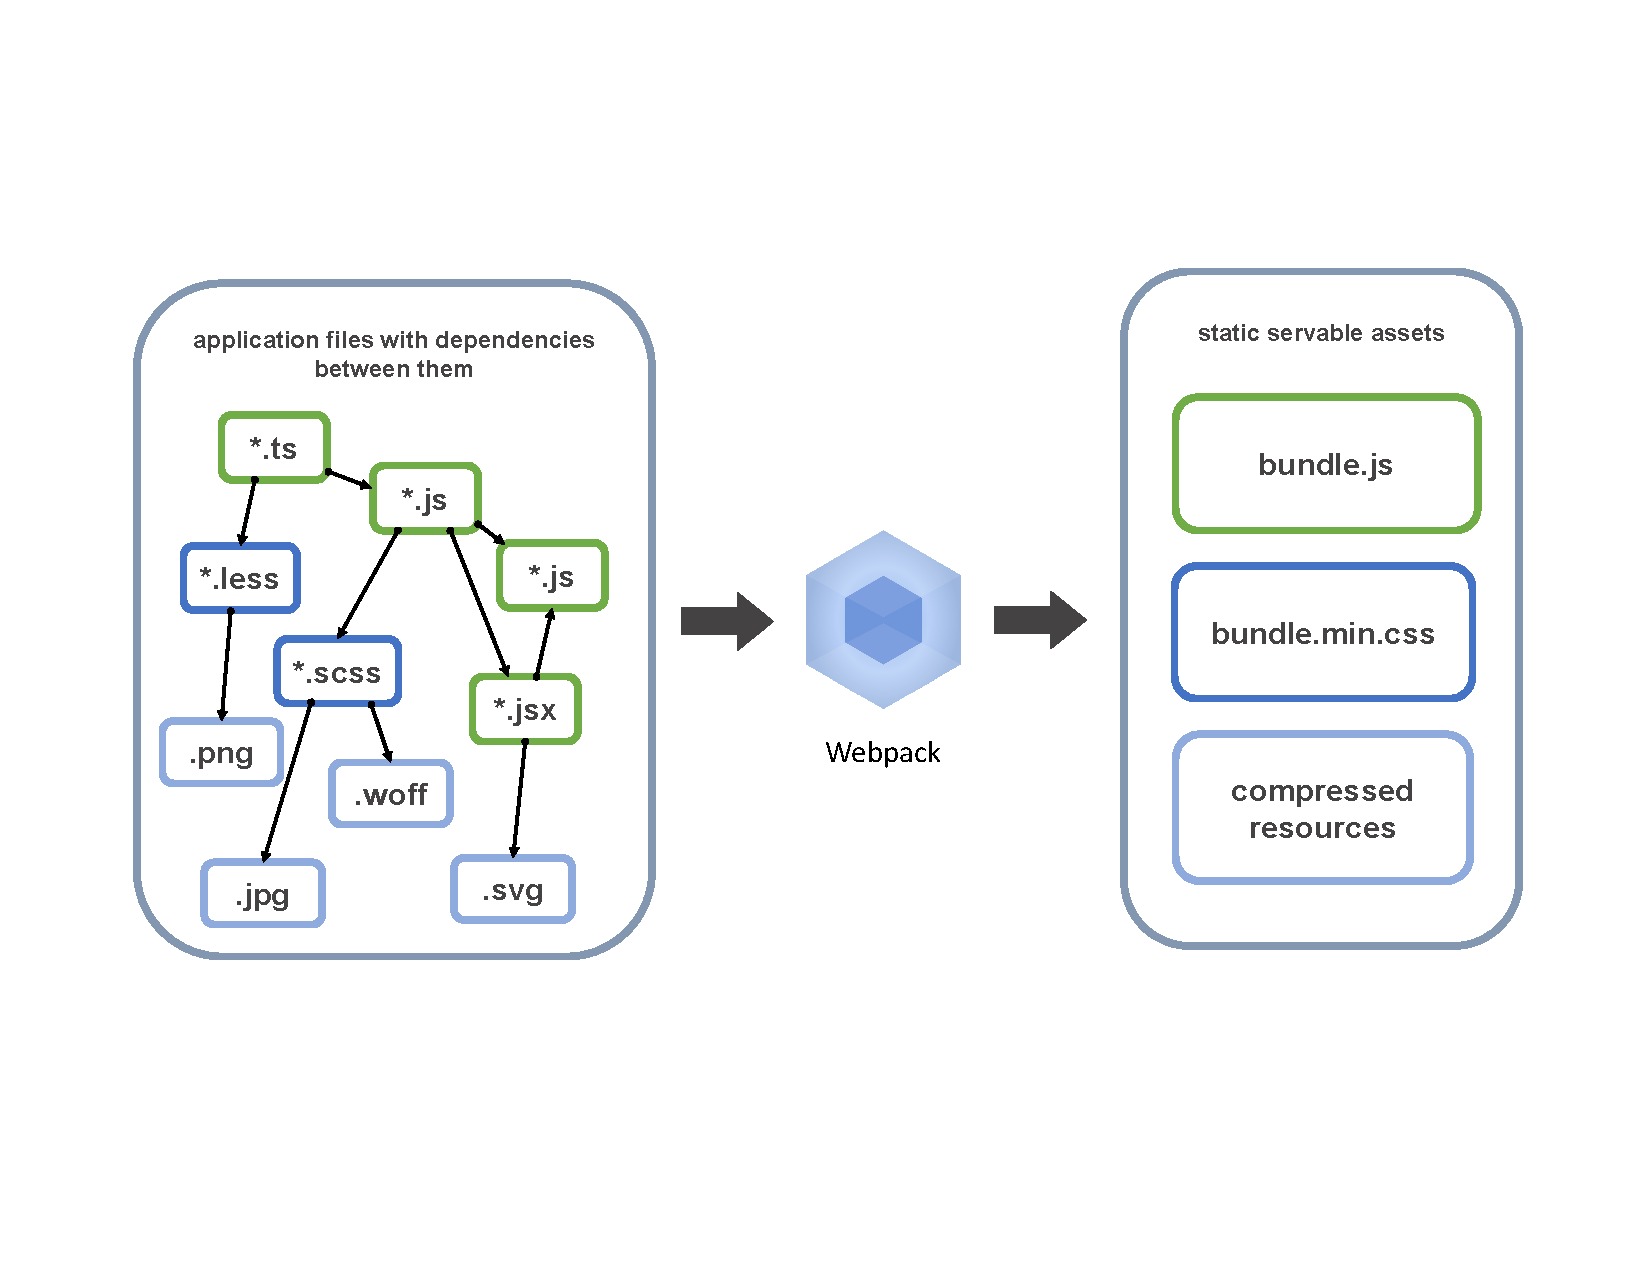
\includegraphics[scale=.6, trim= 2cm 4cm 2cm 4cm, clip]{007webpack.pdf}
  \caption{Webpack transformation visualization}
  \label{fig:webpack}
\end{figure}

\begin{figure}
  \centering
  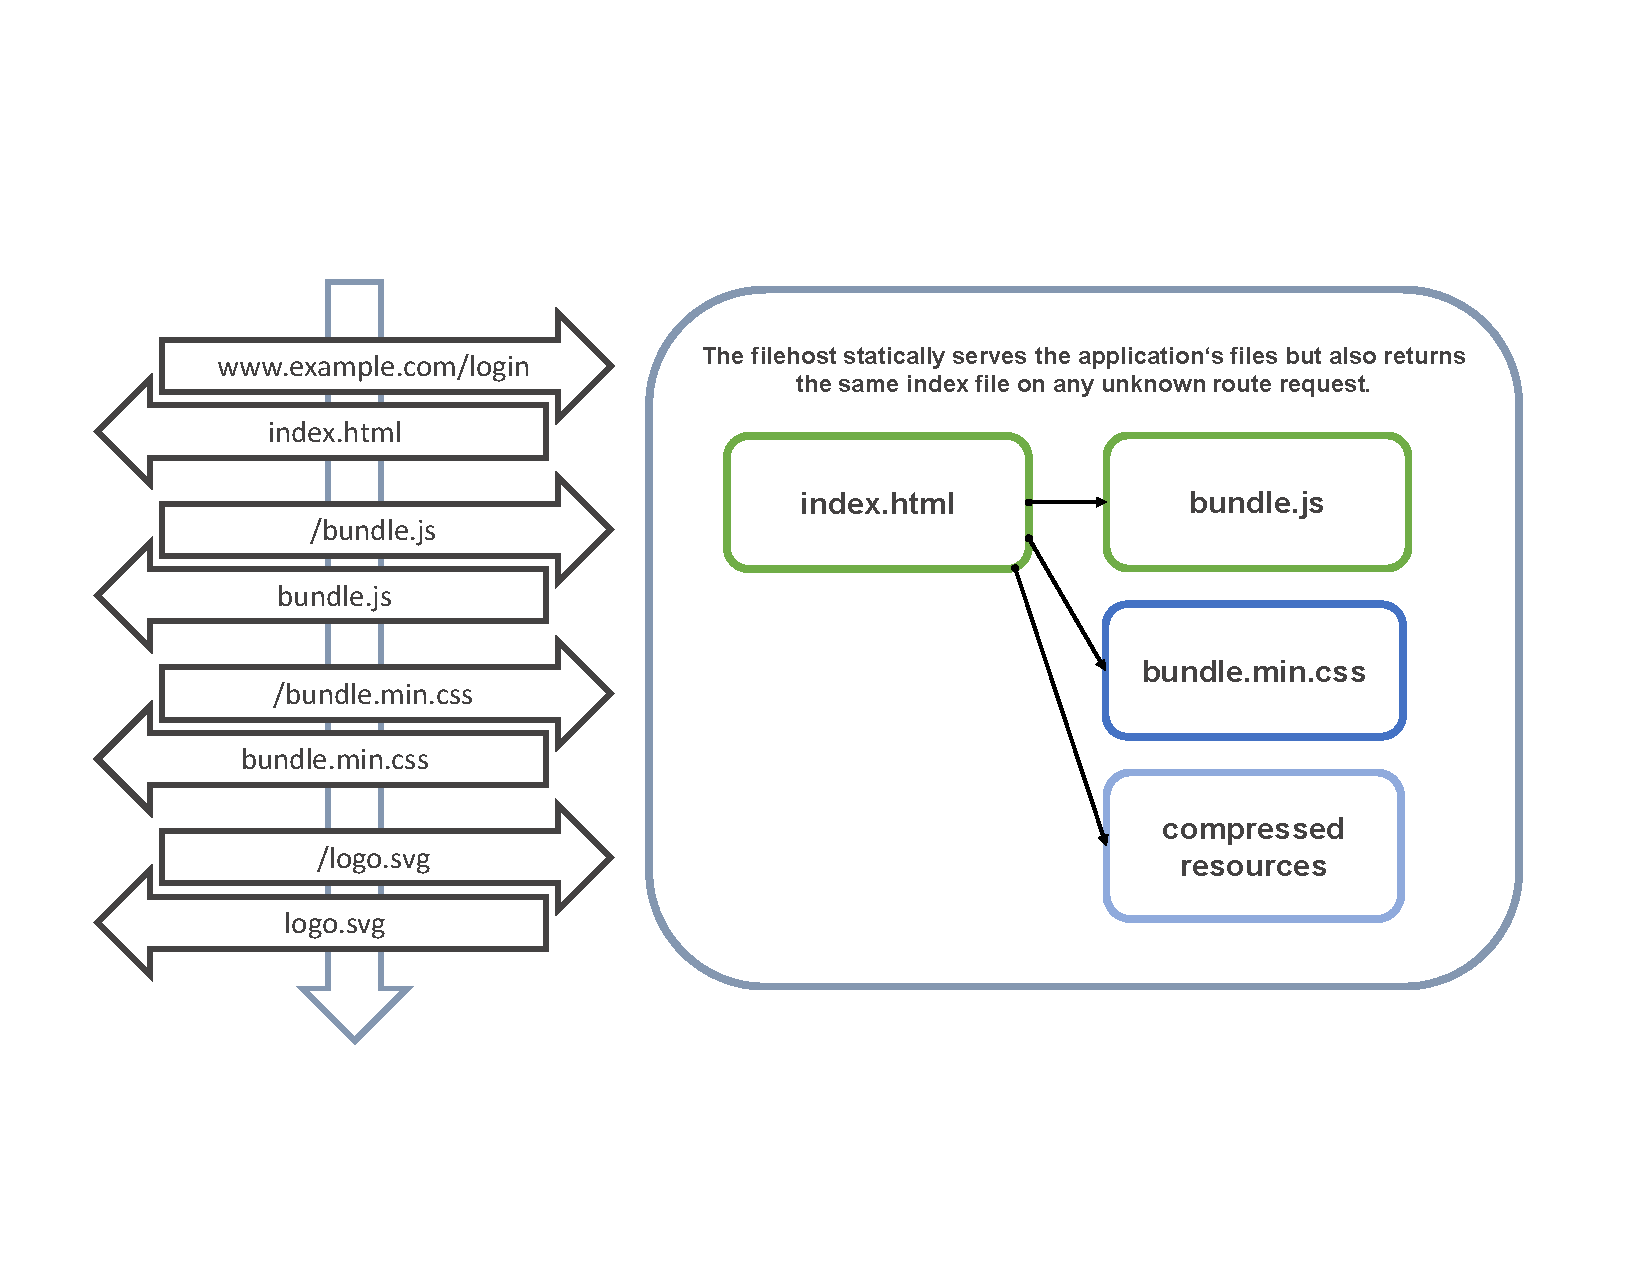
\includegraphics[scale=.6, trim= 1.5cm 3cm 2cm 2cm, clip]{008singlepagedapplication.pdf}
  \caption{Single paged application example}
  \label{fig:singlepagedapplication}
\end{figure}

\mbox{Webpack} is one of the most comprehensive developer tools that can be used for developing a web application using all kinds of files and language flavors. It is a module bundling mechanism that combines all the code base of a project into an application that can be interpreted by a browser. It does not matter if Less, Sass or plain CSS is used, neither does it matter if the project is developed in CoffeeScript, TypeScript or plain JavaScript. \mbox{Webpack's} base functionality is to transform modules with dependencies into static assets as described on the technology's website\footnote{https://webpack.github.io/} and as the example Figure \ref{fig:webpack} shows. 

\mbox{Webpack} is especially useful in combination with the Node Package Manager. Every module that was downloaded by npm can be integrated into the web application with a simple import statement and \mbox{Webpack} does all the work to integrate the module's code into the final bundle. \mbox{Webpack} will handle any dependency in the code and transform it into a code bundle, that includes not only the application's code but also third party module code, that was imported by the developer.

Another outstanding feature is the code splitting and the on-demand-loading of code. Not only is the code bundled and transformed into static assets but also split into code modules again in an intelligent way. Modules that are more heavily used in the application will be loaded first and other less important module parts can be loaded on demand. To avoid client side caching it is possible to include a generated build hash into the modules' name so the browser interprets each module as a new asset that is not yet cached. Deploying updates to an application is therefore no problem.

Many features can be accomplished with \mbox{Webpack} itself, but on top the module bundling mechanism is highly customizable as well. Webpack does support a plugin and loader system that can accomplish even more customization and variety in code transformation. Loaders can load, transform and then return any resource of the code of a web application. An example would be the loading of Sass files and the transformation to CSS. Another use for loaders would be the integration of image files. In the process of loading the images they can also be compressed and are output as static resources. Plugins on the other hand add useful features. One of the most important Plugins for development and production is the \mbox{DefinePlugin}. This piece of code allows the substitution of constants in the application's code according to the environment. With the help of this plugin the app can be run in development or production mode. There are several loaders and plugins provided by the Webpack community that can be downloaded and integrated by npm.

One of the most important features of Webpack for developing React apps is it's own development server. As stated before, NodeJS allows the developer to start a development server, that hot-reloads code parts so the developer does not have to recompile the whole code again in order to see the updated application after a change in the application's code. Not only NodeJS, but especially Webpack enables this feature. The code bundling mechanism enables watching file changes in order to compile changes on the fly and deploy them while the server that serves the front end code is still running. Again, this feature works with any asset of the app, whether it is a CSS file that has changed or a JavaScript file, the hot-loading mechanism is triggered.

When transforming a web application project with Webpack, the outcome is called a single paged application. The term describes a certain kind of web application that is started from one single index file. Most of the work is done by Webpack itself as it already transforms the web application's code into static assets. The server then only has to statically serve all application relevant data. If the requested route does not reference a static asset it means that the client must be requesting a certain page of the web application. In that case the server always has to serve the same index file. By doing that, the requesting client is guaranteed to always get the special index file that bootstraps the whole web application. The application can then react to the current route and display the correct page. The Figure \ref{fig:singlepagedapplication} shows how a request of the login page in a single paged application could look like.

%here i will explain what a one page application is, and how code bundling works with JavaScript imports and so on.

\section{Introduction and overview of the Framework}

Now that it is clear what is needed to set up a ReactJS project and there is a better understanding how the tooling works it is now time to dive deeper into the framework itself. This section will give an introduction to ReactJS and its history. Also basic application architecture will be discussed as well as conventions how to program a ReactJS application. Some core components of the framework will be described to achieve more knowledge on how the library works. 

To begin with, the JavaScript library ReactJS was developed by Facebook. The framework is open source since 2013 but it is still managed by technical engineers of Facebook and is available under a BSD license. The framework itself alows highly component orientated application architecture, which means code parts of a ReactJS application can be used in a very modular way. Once all the boilerplate code is built up and all standard components are implemented, big progress can be achieved in a very short amount of time. The most time consuming part of starting a React web application is to set up all the tooling and all the boilerplate code. To get a better understanding of the framework, some of its components will be explained to then show how a ReactJS application architecture could look like.

Where ReactJS really excels is when it comes to new web technology. The fact that the framework is a descriptive UI defining top-level API makes it easy to use ReactJS for other platforms and technologies as well. When developing a React application top-level highly abstracted simple components can be used that finally get broken down to library function calls that actually create UI elements. ReactJS could be described as a general user interface component abstraction library. Because ReactJS was engineered that way it is easily possible to use React to not only develop web applications but also to use React to develop mobile applications (React Native\footnote{https://facebook.github.io/react-native/}) or build virtual reality environments (React VR\footnote{https://facebook.github.io/react-vr/}) without much effort and without having to learn any new frameworks or programming languages. 

\subsection{JSX} \label{ssec:jsx}

As it can be read in \cite[S.59]{Zeigermann.2016}, \mbox{ReactJS} is a front end framework that does not need a template language to create user interfaces. Instead, the library provides functions to create or manipulate the actual DOM elements of a React component. To make the process of creating elements easier, ReactJS provides a JavaScript language extension called JSX. Code that is written in JSX can be transformed into JavaScript code by \mbox{Babel} and \mbox{Webpack}. 

Using the JSX language extension allows HTML-elemnts to be directly written into the JavaScript application code as this simple example shows. Note that it is necessary to use the JSX notation \texttt{className} instead of \texttt{class} as this is not vanilla HTML. All provided code examples can be tried out in any online live JavaScript editor\footnote{http://codepen.io/gaearon/pen/rrpgNB?editors=0010}. \newline

\begin{JsCode}
const HelloElement = (
  <div className='hello-world'>
    <span>I am a span</span>
    Hello World
  </div>
)
\end{JsCode}

The provided code snippet could not be interpreted by any browser and needs to be transpiled into vanilla JavaScript. The best part about JSX is, that components that are transformed this way are infinitely nestable. Components are easily and infinitely composable that way. ReactJS is a highly component oriented front end framework as mentioned before, making it easy to compose any ReactJS components. After the transformation the code looks like the following code snippet: \newline

\begin{JsCode}
var HelloElement = React.createElement(
  'div',
  { className: 'hello-world' },
  React.createElement(
    'span',
    null,
    'I am a span'
  ),
  'Hello World'
);
\end{JsCode}

The example shows, that the pseudo JSX DOM-elements are transformed into functions from the ReactJS API. The reason why components are infinitely nestable is that they get transformed into plain JavaScript functions that are composed as it can be observed in the example above. Using the functional programming paradigm composition makes it easy to compose any components. The return type is not an actual DOM-element, it is just a lightweight ReactJS JavaScript object but this fact is described in the Section \ref{ssec:VirtualDom} in greater detail. JSX can be tested with any online JSX transpiler like the babel transpiler for example\footnote{https://babeljs.io/repl/}

JSX is one of the most important features of ReactJS because it adds a very important abstraction layer to the view. The developer can use ReactJS components as normal DOM components without knowing the exact implementation. This is also the reason why ReactJS cannot only be used in the web but also for mobile platforms by simply switching the HTML components for the according components of the target platform. An example would be React Native which produces native apps for Android and iOS by using components like \texttt{<View>} instead of the well known HTML element \texttt{<div>} for example.

\subsection{Components and properties}

JSX is not only used to create common HTML elements, it can also be used to make use of components that were programmed by the developer. These so called \enquote{React components} can be JavaScript classes that extend the React \texttt{Component} class or pure functions as described in Section \ref{ssec:PureFunctionalComponent}. There was also the approach to use the React class factory function \texttt{React.createClass()} to use OOP style components in JavaScript. As the ECMAScript introduced the class syntax the class factory function was deprecated as it is better to use native classes than functions that get used as classes with the help of their closure. In the most cases components are functions or classes that can be used as a JSX element as shown in this example: \newline

\begin{JsCode}
class Hello1 extends React.Component {
  render() {
  	return <div>Hello, World!</div>
  }
}

const Hello2 = () => <div>Hello, World!</div>
\end{JsCode}

Note, that the anonymus function is declared as a ES6 \enquote{fat-arrow function}. Basically the \texttt{Hello1} and \texttt{Hello2} variables act identically. When rendered, they show the exact same output but have no functionality attached to them. The following example shows, how the newly created React components can be used with JSX: \newline

\begin{JsCode}
ReactDOM.render(
  <Hello1/>,
  document.getElementById('container1')
);

ReactDOM.render(
  <Hello2/>,
  document.getElementById('container1')
);
\end{JsCode}

The name of the component object defines the JSX element name. The two ReactJS API functions (\texttt{ReactDOM.render()}) will search for elements in the HTML-DOM that are called \enquote{container1} and \enquote{container2} and render the two React components instead of them. Usually, the \texttt{ReactDOM.render()} function is only used once in a ReactJS web application as a bootstrapping mechanism to set one element as the application root so ReactJS can build its actual DOM tree onto the specified element. As mentioned before, ReactJS components are infinitely nestable so there only has to be one actual root element in the real HTML-DOM to bootstrap onto.

To add functionality to a component it can be accomplished by passing it so called \textit{props} and processing them with JavaScript component logic. Passing a prop is really easy in JSX:

\begin{JsCode}
const HelloComponent = (props) => {
  props.ownFunction('this will get logged')
	return (
 		<div>
    	<h1>{props.title}</h1>
      {props.text}
		</div>
  ) 
}

ReactDOM.render(
  <HelloComponent title='Hello' text='World!' ownFunction={console.log} />,
  document.getElementById('root')
);
\end{JsCode}

\begin{figure}
  \centering
  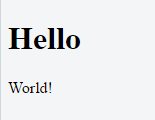
\includegraphics{001HelloComponent}
  \caption{Output of rendering HelloComponent}
  \label{fig:HelloComponent}
\end{figure}

The output of this snippet of code can be seen in the Figure \ref{fig:HelloComponent}. A very useful feature of JSX is that also functions can be passed to a React component. This is very useful when nested child components have to trigger logic in their parent component.

\subsection{Stateful components in ReactJS}

The component logic is very important in React. Functionality can be added by adding member functions to ReactJS class components to manipulate received props and providing a view to the provided data. Like discussed before, there are React components that are functions but there are also React components that extend the class \texttt{React.Component}. These classes do have a lifecycle and their own component state which can be manipulated as well. These class components produce more overhead as React treats these class components as smart components with state and lifecycle that has to be handed accordingly. Class components should only be used where it is absolutely necessary to reduce overhead and improve performance.

Lifecycle methods are very important if the component has to handle any asynchronous task or if incomming props have to be mutated. All the available methods are documented in the official documentation \cite[Docs: React.Component]{FacebookInc.2013}. For example there are methods that get executed before the component is about to mount (\texttt{componentWillMount()}), when it receives its props (\texttt{componentWillReceiveProps()}) or when it is about to unmount (\texttt{componentWillUnmount()}). The most important lifecycle method is the \texttt{render()} method though. This method gets called when the component has received its props and state and is about to render the view to the user. According to the documentation, API calls should be handled in the \texttt{ComponentDidMount()} method. The reason for that is to improve user experience. All components should render with an initial state and update themselves accordingly when asynchronously fetched data arrives. Another very important lifecycle method is the \texttt{shouldComponentUpdate()} method. The purpose of this method is to being able to exactly define the data that has to change in order to trigger the \texttt{render()} function. By overriding this method performance can be increased greatly because unnecessary rerendering cycles of the component that would otherwise slow down the whole application can be prevented.

Class components also have their own state that can be mutated by the member method \texttt{setState()}. As mentioned before, Facebook claims ReactJS does not make any assumptions about the development stack. This does also include the fact that ReactJS does not assume that the developer uses any form of application state container by him- or herself. This is the reason why ReactJS class components can have their own state which is tied to all the lifecycle methods. When either the component's state or props change the component will go through the according lifecycle methods including the \texttt{render()} method and is therefore rerendered. Class components are also often called \enquote{stateful components}.

The following code example shows how a stateful component could look like. Note that it is still possible to pass props to the stateful component. React makes use of the ECMAScript class syntax and extends the \texttt{React.Component} base class for creating stateful React components.

\begin{JsCode}
class StatefulComponent extends React.Component {
  
  constructor(props) {
    super(props)
    // setting the initial state in the constructor
    this.state = {
      value: 'initial'
    }
  }
  
  mutateState(value) {
    // mutate state with React Component method to trigger lifecycle methods
    // this method is asynchronous
    // any asynchronous action can be performed like calling an api
    this.setState({ value })
  }
  
  componentDidUpdate() {
  	console.log('i was updated')
  }
  
  render() { 
    return (
      <div>
        <button onClick={this.mutateState.bind(this, 'mutated!!!')}>Mutate Me</button>
        <p>{ this.state.value }</p>
      </div>
    )
  }
}
\end{JsCode}

When executed, a button and a text field (paragraph tag) are shown. Initially the text renders as \enquote{initial}. Once the button is pressed, the internal state of the component changes and it renders \enquote{mutated!!!}. Every time any props or state changes, the React component reiterates all lifecycle methods that are implemented. In this example the \texttt{ComponentDidUpdate()} method gets executed after each time the button was pressed because the state of the component changed by executing the \texttt{setState()} method.

%% achitecture -> 

% maybe show an example of smart component?
% "smart" and "dumb" components

\subsection{Pure functional components} 
\label{ssec:PureFunctionalComponent}

The other type of components ReactJS has to offer are so called \enquote{functional components} or \enquote{stateless components}. This type of component is often used to render parts of the application that do not have any component logic attached to them. Functional components are only a declaration of how the component has to look at a certain state. These components receive the application state via props and can also trigger logic operations by invoking functions that were passed as props as well. Functional components are often called \enquote{dumb components} because their only reason of existence is to provide a view to a certain application state.

When seen in the perspective of functional programming one could also call these components pure functions. The fact that the functions are pure without any side effects make the components easily testable. Functional components are pure functions that will always produce the same view for the same constellation of props. React does \emph{not} treat these dumb components as a stateful component. That is the reason why there is no additional overhead as the JSX component gets transformed into a simple \texttt{React.createElement()} call as it can be seen in the examples above. Neither lifecycle nor component state has to be considered by React when using pure functional components which greatly improves performance and reduces script execution time overhead. 

The following code snippet is considered a functional component. Components like buttons or text input fields are perfect for being a functional component as they will get used very often throughout the whole application.

\begin{JsCode}
const FunctionalComponent = (props) => (
  <div>
    with the same props i will always render the same...
    {props.text}
  </div>
)
\end{JsCode}

The only constraint of functional components to be used in conjunction with JSX is, that they have a capital letter at the beginning so JSX recognizes the function as a React component. The component can then be used very easily in JSX as the following snippet shows:

\begin{JsCode}
<div>
  <FunctionalComponent text='I am so pure!' />
<div>
\end{JsCode}

% "dumb" components only function, only view

% \subsection{React Router}

% components with logic, after that only functional components
% routing of the app, hash routing, react router breaking changes every few months

% \subsection{Styling}

% is this really necessary, maybe covered in webpack section?

\subsection{Property Types}

JavaScript is a dynamic typeless scripting language. Because of this very reason ReactJS provides an API that lets developers specify property types for each component. When React is executed in the development mode each component will check the provided property types to ensure that the component is used correctly. The following example shows how the so-called \texttt{PropTypes} can be used:\newline

\begin{JsCode}
const Component = (props) => {
  
  // if the prop title is not set it gets set to a fallback value
  // the prop is not guaranteed to be set so the programmer has to implement a fallback
  const title = props.title || 'I am the standard title'
  
  // the callback property is guaranteed as it is set to isRequired
  // if the text prop is not set the defaultProps object will set it
  return (
    <div>
      <button onClick={props.callback}>Button</button>
      <p>{props.title}</p>
      <p>{props.text}</p>
    </div>
  )
}

Component.propTpyes = {
  title: PropTypes.string,
  callback: PropTypes.func.isRequired,
  text: PropTypes.string,
}

Component.defaultProps = {
  text: 'i am the default text'
}

\end{JsCode}

The \texttt{propTypes} and the \texttt{defaultProps} objects are static and can be assigned to statful \emph{and} stateless components. The \texttt{propTypes} can be used to specify which property has to be of what type and to specify which component is required. To read about the full potential of \texttt{PropTypes} it is advised to have a look at React's documentation (\cite[Typechecking With PropTypes]{FacebookInc.2013}). The \texttt{defaultProps} object can be used to set props to a default value if they are not set by the user of the component. By doing this the developer of the component does not have to implement fallback solutions if the property is undefined.

It is important to note that the property check is disabled when ReactJS is bundled in production mode as the type checks are only viable during the development of the application and introduce scripting overhead. The default properties on the other hand get set even when the production mode is enabled.

\subsection{Virtual DOM} 
\label{ssec:VirtualDom}

% makes react very fast
% dom operations expensive
% javascript object light weight and fast
% diffing algo and reconciler
% renderer pluggable

The most expensive operations when it comes to rendering anything in the browser are DOM manipulations by JavaScript. React solves this problem by using a concept named \enquote{Virtual DOM} or \enquote{shadow DOM}. As stated in \cite[Docs: Reconciliation]{FacebookInc.2013} ReactJS is a declarative framework that allows the user not having to think about the changes that have to applied to the current built up DOM elements. When using frameworks like jQuery, DOM elements have to be referenced directly in order to manipulate them. ReactJS on the other hand builds up its own Virtual DOM which is a plain old JavaScript object, calculates any changes with its built in diffing algorithm and applies possible changes to the DOM making the framework very fast. Instead of having to tell the browser what elements to update it is possible to tell React how the application should look like at any given state (declarative) as it can be heard in \cite[1:50]{youtube.2017}. This mechanism is called the \enquote{reconciliation algorithm} and is a part of the core algorithm of React.

Internally using a Virtual DOM is not only useful in the web where there is an actual DOM but also in other hardware environments as stated in \cite[2:10]{youtube.2017}. Facebook decided to divide the diffing algorithm and the part of the code that actually handles pending changes in the DOM which led to the distinction between the \enquote{renderer} and the \enquote{reconciler}. The renderer was transformed into a pluggable part of ReactJS enabling the framework to be available on other platforms as well. React Native for example is a ReactJS framework that makes it possible to produce mobile applications that can be compiled for Android and iOS by simply switching out the renderer part of the ReactJS core algorithm.

% \subsection{React Fiber} \label{sec:reactfiber}

% talk about how virtual dom is outdated and fiber will win

\section{Redux}

In Chapter \ref{cha:fluxreduxmvc} the programming pattern Flux was introduced. In the early days of ReactJS, Flux had to be implemented by the developers themselves because there was no framework that could handle application state management by using the Flux pattern at the time. To encourage developers to use the Flux pattern the Redux framework was born in May 2015 which can be researched in \cite{DanAbramov.2015}. The library is basically a state container that is designed with the Flux application architecture in mind. Redux can be used for any application but it suits very well to be used in conjunction with ReactJS. If the reader decides to utilize the Flux architecture to program a web application, it is definitely a good idea to use Redux. The library makes it exceptionally easy to develop an application with the new paradigm in mind and takes the overhead of having to design a Flux architecture by the programmer away.

% what is redux and why does it exist and how does it make web development easier

\subsection{Introduction and overview} \label{ssec:introductionoverview}

With Redux it is very easy to implement a global state on any front end application. Like the Flux design, Redux also consists of components like the Action and the Store component with a Dispatcher handling incoming actions. Redux is a little bit different than Flux though. Like explained in the Section \ref{ssec:fluxstore}, Flux can have multiple stores that can be registered via a callback. Redux only has one store and achieves this by composing all stores into one store. The goal is, that actions can be dispatched onto the store resulting into a mutated state that can then be set and passed to any connected ReactJS component.

% describe actions with code example
Like described in Section \ref{ssec:fluxaction}, an Action can be created by any user interaction and has to be dispatched to the store. As it can be read in \cite[Actions]{DanAbramov.2015} an action has to return an Object containing all necessary information for the reducer which will be introduced in the next section. An example of an Action could be the following code snippet:

\begin{JsCode}
const mutateStoreData = (data) => {
  return {
    type: MUTATE_DATA,
    data,
  }
}
\end{JsCode}

As per default, it is rather complicated to perform asynchronous operations in an Action. The documentation \cite[Async Actions]{DanAbramov.2015} suggests to use a middleware (redux-thunk\footnote{https://github.com/gaearon/redux-thunk}) that allows actions to have a callback to perform asynchronous actions. An example could be the following code snippet:

\begin{JsCode}
const asyncMutateStoreData = (params) => (dispatch) => {
  doSmthAsync(params, (error, data) => {
  	// this is the callback function context of doSmthAsync 
    // it gets called once the async operation is complete
    // this could be a file system operation or an API call
    if (error) throw new Error('error')
    // the dispatch callback can be used to resolve asynchronously
    // data from the action can be dispatched to the store at any point in time
    dispatch({
      type: MUTATE_DATA,
      data,
    })
  })
}
\end{JsCode}

The so called \enquote{Reducer} is a very important aspect of Redux as it can be read in \cite[Reducers]{DanAbramov.2015}. The reducer is responsible for taking the store's data, changing it by using a pure function that takes the current state and an action and returns the newly calculated state. It is of utter importance to understand, that the state is \textbf{not} mutated. The newly evaluated state is then set as the new current global state. This makes applications very easy to debug because there are no side effects in the reducer as it is a pure function. There is even a tool\footnote{https://github.com/gaearon/redux-devtools} which can restore any previously set states of the store, creating the possibility to \enquote{time travel} through all different versions of the application state. It is exceptionally easy for the developer to restore any previously set state which increases the debugability of the application greatly.

The following code example shows how a reducer function could look like:

\begin{JsCode}
const reducer = (state, action) => {
  switch(action.type) {
  	
    case MUTATE_DATA:
      state.data = action.data
      return state
  
    default: 
      return state
  }
}
\end{JsCode}

% reducer code example
% maybe insert a graphic here?? or next section? maybe show redux dev tools?

\subsection{Connection to ReactJS}

Redux is very often used in conjunction with ReactJS. According to the statistics of Sacha Greif \cite[Front-End Frameworks]{SachaGreif.2016} about 60\% of developers that use ReactJS also use Redux for state management. To use Redux with React a package named \texttt{react-redux}\footnote{https://github.com/reactjs/react-redux} has to be used in order to connect React components to the Redux store. The react-redux package provides a \texttt{connect()} function that can be used to compose a React component that is intended to be connected to the store.

It was promised before to show why Flux-Redux works well with React. The reason why Redux is perfect for React is, that the application state is passed to a component as a prop. As the reader should know by now, React components only update when either props or the state change. Through the react-redux package certain parts of the state can be mapped to a component only causing rerenders when the corresponding prop that was mapped from the state changed.

The following code example shows how easy it is to map the stores state to a component. The \texttt{connect()} function takes a state mapping function as a parameter. The \texttt{connect()} function is composable and therefore has to be invoked a second time by passing in the component that has to be connected to the store. The first invocation of \texttt{connect()} returns a function that will take either a stateful or stateless component. The code example also shows how to dispatch an action to the store. When composing a component with the \texttt{connect()} function, the \texttt{dispatch()} function automatically gets added to the props of the connected component. \newline

\begin{JsCode}
const mapStateToProps = (state) => {
  const { dataToExtract } = state
  return { dataToExtract }
}

const MyComponent = (props) => {
  // this component can access the store's current state
  // every time the mapped state changes, this component will rerender
  return (
    <div>
      <button onClick={() => this.props.dispatch(mutateStoreData('mutated!!!')}></button>
      {props.dataToExtract}
    </div>
  )
}

// this is where the magic happens and where the component is connected
export default connect(mapStateToProps)(MyComponent)
\end{JsCode}

% CODE EXAMPLE with connect
% how can redux be connected to react js
% component tree updates

\subsection{Immutability of the store's data}

Probably the most important aspect to consider when using Redux with ReactJS is to use a library that makes the Redux's store data immutable. Immutability is a very complex topic when programming applications with JavaScript. As a developer you can never be sure what operations mutate the objects and what functions clone the object and return the mutated object as the function's result. There are several packages that can be used to make the store's data of Redux immutable, like the \enquote{seamless-immutable} package. These immutability libraries ensure the programmer that a JavaScript object created by any chosen immutability library cannot be mutated directly. It has to be done by using the libraries API or by creating a new object.

The question that arises is: \enquote{Why is immutability so important when using Redux?} The answer to that question is very simple: Once React applications get very big, performance can be a serious problem if too many rendering cycles happen at the same time. ReactJS provides an API to check if a component should be updated or not. This is usually handled by a shallow comparison of the objects or can be implemented by the developer by overriding the lifecycle method \texttt{shouldComponentUpdate()}. When mapping a whole component tree to the component, a shallow compare will not be sufficient to note any changes in the JavaScript state object if it was changed deep down in the object tree. The solution to this problem would be a deep compare but having to iterate the whole state object tree can be a very expensive operation in addition to a complete rerender of the component. 

If many state changes occur in a very short amount of time the comparing function has to be executed on every prop or state change. That is the very reason why the comparing function should be as performance efficient as possible. With an immutable object the comparison function can just directly compare the objects which is an extremely cheap JavaScript triple equals comparison. The object cannot be mutated by a simple JavaScript operation and once the state has to be mutated it has to be done by the immutability library or by creating a new object. Either one of these cases cause the JavaScript triple equals comparison to not return true therefore causing a rerendering cycle. If the previous and the current state object are equal the component knows that the state has not mutated and will not rerender.

In the Section \ref{ssec:introductionoverview} a code example of a possible reducer was shown. In that example the object is mutated directly by accessing a property of the store object. In JavaScript mutating an object by accessing a property does not mutate the whole object but only that property. To notice any changes the object cannot be compared by JavaScript's triple equals operator but one would have to write a deep comparison function comparing all properties of the object. When using immutable objects the object itself knows when it was mutated even if the mutation happened deep down in the object tree making the comparison with the triple equals operator possible again.

As the time of writing this, ReactJS is in the version 15.5.4. This version not only provides a \texttt{React.Component} base class to extend from, but also a \texttt{React.PureComponent} class that automatically implements the \texttt{shouldComponentUpdate()} method. This special component achieves this by automatically shallow comparing all current props with every new incomming prop. When using an immutable store this component type gets highly useful as the programmer does not have to implement the \texttt{shouldComponentUpdate()} method.

% \subsection{Asynchronous store}

% make javascript even more scalable by making even state changing actions async and let the script language engines decide when to execute the actions and thus increase performance

\subsection{Advantages and disadvantages of using Flux-Redux}

Probably the biggest advantage of using Flux-Redux in any React application is the possibility to store a global application state that lives as long as the user is actually using the web application. This can improve user experience greatly. A good example would be the possibility to being able to trigger a function that displays an error modal from any part in the application. The modal's state could be \texttt{\{ visible: true \}} which tells it to be displayed no matter what state the rest of the application is in and what screen component is displayed at the time of triggering the function. Another good example would be user input. The user inputs some form data but changes the view causing different components to be displayed. Once the user comes back to the form component the state is still saved in the Redux store.

A big disadvantage is the amount of boilerplate code that is necessary to create actions and reducing functions. Once the programmer decides to divide the application into more than one store all of these stores have to be somehow composed before they can be used by the Redux library. The framework has an API that lets programmers compose stores and middlewares but it is still boilerplate code that costs time.

Once there is a part of the app that needs to store state in any store several steps have to happen that cost time and programming overhead as well. First an Action has to be implemented that possibly handles API calls and prepares some data for the store. An action constant has to be created as well in order to being able to dispatch the action to the stores. The action constant is the action type that gets parsed in the store's reducer function to decide how to reduce the data. Finally, the corresponding reducing function in the store has to be implemented. Once all of these components are finished they somehow have to be connected to the ReactJS component that will utilize the newly implemented logic. As mentioned before, the package \texttt{react-redux} provides an API to compose any React component to be connected to the store. In order to being able to do this mapping functions have to be written that not only map the store's state to the components props but also maps the corresponding actions to the props of the component so that they can be used inside the component. The programming overhead can be considered as big disadvantage but it guarantees unidirectional dataflow, debugability, scaleability, and testability of the application.

%% any code examples of creating store? any graphs?

\section{Application Architecture} \label{sec:application-architecture}

Now that the reader is a more familiar with React's concept of stateful and stateless components and knows more about how to store application state efficiently it is time to talk about best practices to build well performing and scaling ReactJS web applications as promised at the beginning of this chapter. Of course there are no definite best practices, this paper is based on personal research and personal experience. The reader is invited to evaluate every suggestion him- or herself and form his or her own opinion.

In most cases it is the best practice to think about the fundamental application architecture before starting the project. The application should strictly be divided into smart and dumb components. Currently a community standard is arising that divides web applications into pages (smart components) that handle all the application logic that is relevant for the page and components (dumb components) that can be reused throughout the whole application. Good candidates for stateless components would be a button with a certain style attached to it or a component that can handle page layout. Instead of using native DOM elements every application should reach a point in time where the development of stateless components allows to construct a page by using only own components from the existing component directory.

If there is the need to use a stateful component use the \texttt{PureComponent} base class from the ReactJS API or the \texttt{shouldComponentUpdate()} lifecycle method. It is always a good idea to carefully consider what prop and state changes should cause the component to rerender. Nevertheless, using stateful components should be avoided where ever possible. The best practice would be to only have one parent component that implements all the component logic via member methods and passes them down to all children. The application is much easier debugable because there is only one component where logic is executed and where the data comes from.

Never map child components to the Redux store. The best practice is to only connect page components to the store and pass all relevant data and functions as props to the child components as mentioned before. By strictly following this best practice the structure of the application is much easier understandable and readable. The code base gets more maintainable as new contributors exactly know where all the logic operations happen and where data comes from. When also connecting child components to the store the code base can get very confusing and it is harder for the developer to prevent unnecessary component rerendering cycles.

\begin{figure}
  \centering
  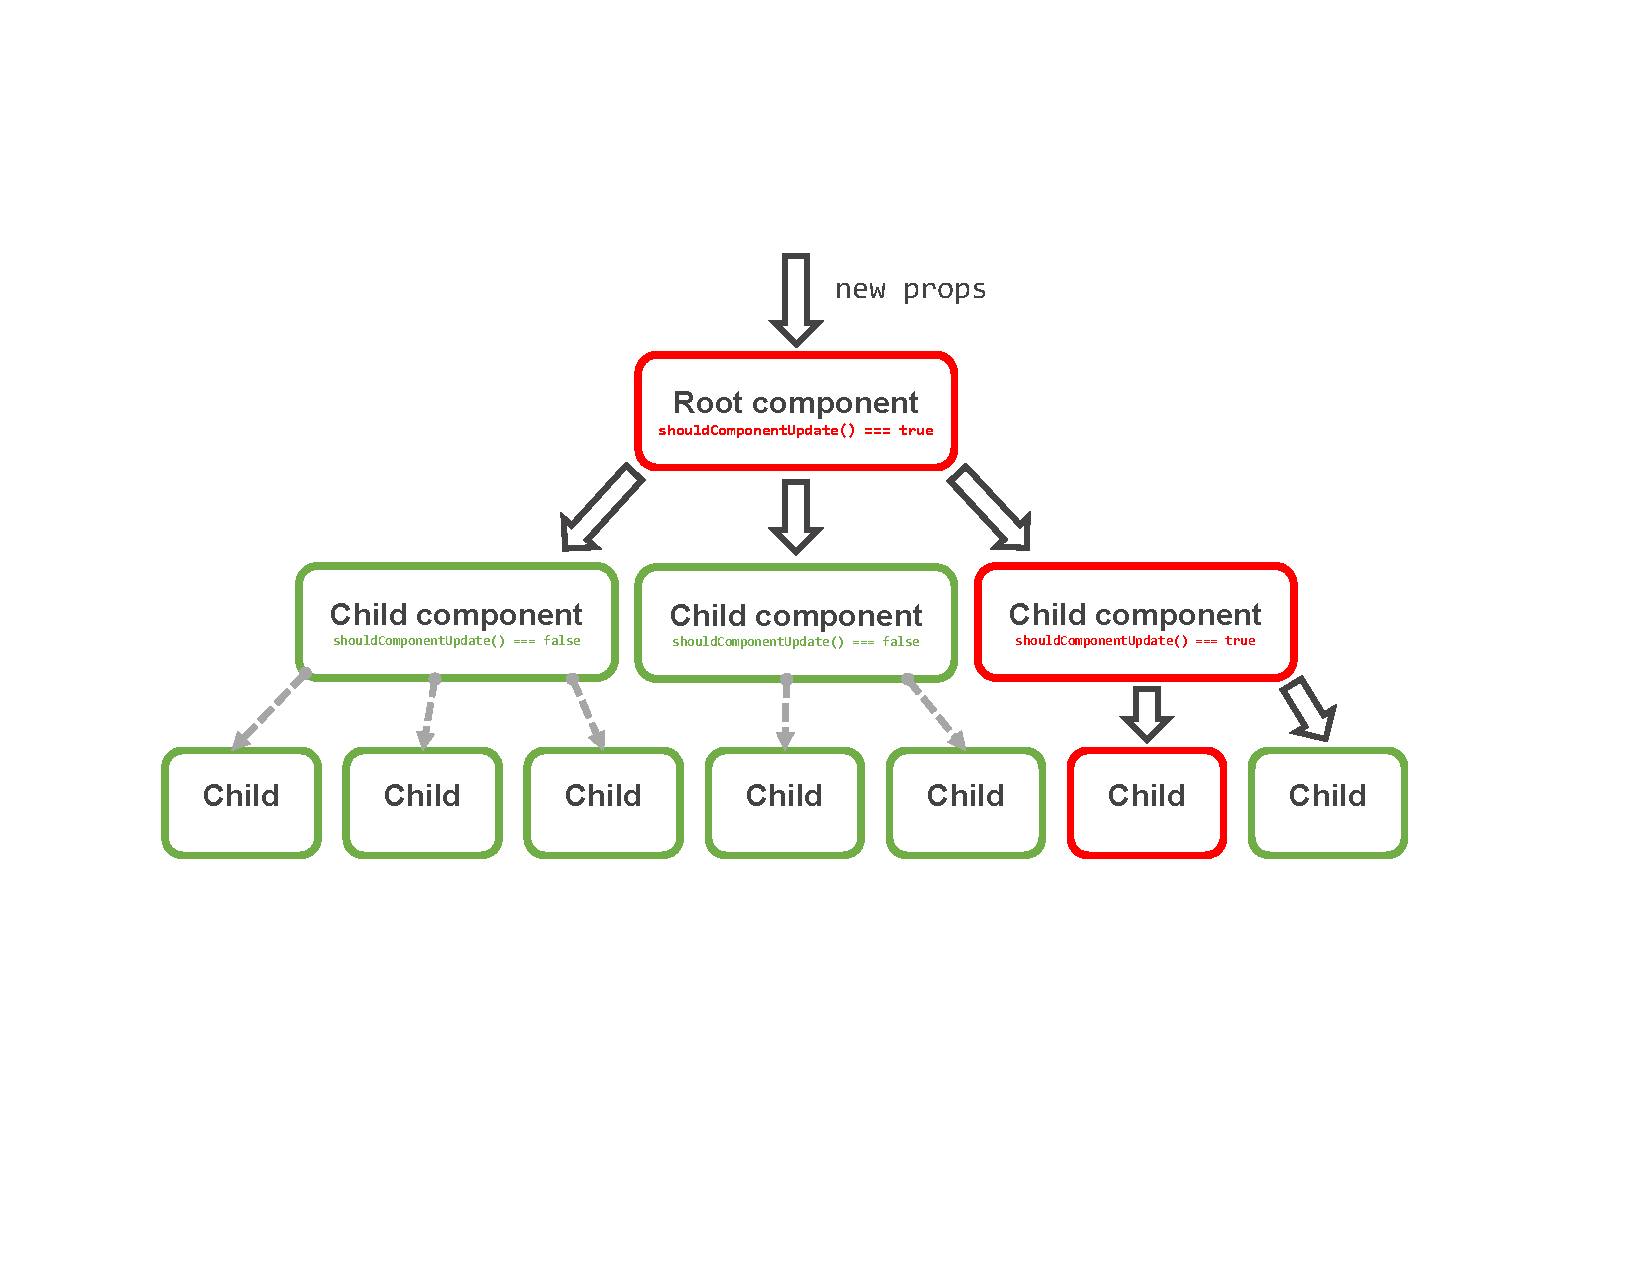
\includegraphics[scale=.7, trim= 2cm 6cm 2.5cm 3cm, clip]{009reactupdatecycle.pdf}
  \caption{React render cycle chain example}
  \label{fig:reactrerenderchainexample}
\end{figure}

Another advice is to split the application into logical component sections. In ReactJS child components only rerender if their parent components went through an update cycle thus changing the child component's props. To prevent massive rerendering chain reactions it is only necessary to prevent a parent component from rerendering (either by using React's base class \texttt{PureComponent} or by implenting the \texttt{shouldComponentUpdate()} method) and a side effect of this is that none of its child components will rerender neither as it can be observed in the Figure \ref{fig:reactrerenderchainexample}.

Use the new fat arrow syntax of ES6 as it makes the code look more clean and also resolves the problem of binding the correct context to utility functions that have to be passed to child components. The following code example will show the difference between the different approaches and how the code can be kept clean by using fat arrow functions: \newline

\begin{JsCode}
const ChildComponent = (props) => {
  return (
    <div>
      <button onClick={props.action}>will cause error</button>
      <button onClick={props.correctlyBoundAction}>will mutate state</button>
      <button onClick={props.oldWayOfBindingAction}>will also mutate state</button>
    </div>
  )
}

class ParentComponent extends React.PureComponent {
  
  constructor(props) {
  	super(props)
    // this is ugly boilerplate code
    // it was necessary before fat arrow functions were introduced with ES6
    this.oldWayOfBindingAction.bind(this) 
  }
  
  action() {
    // when executed in the child component this is undefinded -> error
  	this.setState({ value: 'mutated' })
  }
  
  correctlyBoundAction = () => {
    // through the arrow function the this context is correctly bound to the function
  	this.setState({ value: 'mutated' })
  }
  
  oldWayOfBindingAction() {
    // this context is bound in the constructor
  	this.setState({ value: 'mutated' })
  }
  
  render() {
  	return (
      <div>
      	<ChildComponent
          action={this.action}
          correctlyBoundAction={this.correctlyBoundAction}
          oldWayOfBindingAction={this.oldWayOfBindingAction}
        />
      </div>
    )
  }
}
\end{JsCode}

Experience shows, that sometimes it makes sense to swap out functional components with classes that extend the \texttt{PureComponent} base class. It makes the component a stateful component that has to go through all lifecycle methods but in some cases where a big amount of data has to be passed to a component or the component is expensive to render it sometimes makes more sense to use a \texttt{PureComponent} than a pure function to prevent unnecessary rerendering cycles.

It is strongly advised to implement the \texttt{propTypes} object of every component. By doing so the application is easier to understand for developers that are new to the code base. Developers who want to use or debug any specific component can easily check what properties exist for the component and what properties are mandatory to being set. This increases the process of understanding each component's logic even if the code is rather complicated.










\chapter{Prototype "Julep Search"}
\label{cha:prototypejulepsearch}

In this final chapter of this thesis the reader will be introduced to the prototype that was developed during the research time of this paper. The understanding of all topics that were presented in this thesis should be greatly improved by going over an actual practical example of a real world ReactJS web application. Many best practice and application architecture suggestions are based on the practical experience that was collected during the development of the prototype.

\section{Introduction to the project}

First there will be an introduction to what Julep Search actually is about and what the tool is trying to achieve. This prototype partly was developed while working in an internship at a small web agency in Vienna which is called \enquote{Agentur Mint}\footnote{https://www.agentur-mint.com/}. One branch of this company called \enquote{Mint Square}\footnote{https://www.mint-square.com/} is supporting companies with programmatic advertising know-how and and consultancy. The prototype which is presented is a tool which was built for this branch of the Mint agency to alleviate the tedious process of searching large databases for client specific programmatic advertisement data.

\subsection{Motivation}

Mint Square actually has a database for many different advertising platforms and at one point in time there was the need for a tool that could sort and visualize large amounts of raw advertisement information data. That data can be used to optimize the placement of advertisements and help companies to specifically put advertisements on spots that are most relevant to be noticed and realized by the users. This process is called \enquote{programmatic advertisement}.

The motivation is to easily process programmatic advertisement data  that can then further processed by the collaborators of the Mint-Square team. The most important requirement is to make all data searchable by embedding data into an interface that is easily operable.

\subsection{Usecase}

Once a company wants to start using programmatic advertising for their web appearance it is necessary to get some information what kind of advertisement would work best in what kind of situation. The target audience has to be evaluated and also what advertisements would work best for that audience. This tool queries a large database for all kinds of key information. For example there are queries for keywords, categories, or inventories. The results then show the corresponding advertisement providers, their request counter and additional information that can be used by the employees of Mint Square to evaluate whether the advertisement provider is valid or not.

\subsection{Used technologies} \label{ssec:usedtechnologies}

The application itself is a staticly served single page application built with ReactJS. It is hosted on an Amazon S3 bucket, which is a simple static file hosting server that is extremely cheap to operate. As it was explained before in this paper, bundling a web application by technologies like Webpack makes it easy to host the application on any platform as only static files have to be served to the client.

The database that contains all relevant advertisement data is an Amazon Elastic Search container\footnote{https://www.elastic.co/}. Elastic search is a database that makes querying data with special context very easy. It has a built in matching percentage algorithm that lets the programmer query the most relevant data and also sort the data after its relevancy.

Julep Search does not need a back end server other than its database. For this project a serverless\footnote{https://serverless.com/} approach was chosen. Serverless is a technology that makes heavy use of Amazon's lambda functions completely omitting the necessity to operate a server for any API calls. Lambda functions won't be explained in this paper as it would go beyond the scope of this paper. Information about Amazon's lambda functions can be read on Amazons official documentation\footnote{http://docs.aws.amazon.com/lambda/latest/dg/welcome.html}.

\section{The prototype}

When designing the prototype the most important goal was to implement a ReactJS web application that conforms to all best practices at the time (summer 2016). The emphasis was to have a code base that is easily readable and maintainable once the project is not actively maintained by the initial developer anymore. This section will give a quick overview over the most important aspects of the prototype and explain all thought and architectural decisions that were made.

\subsection{Architecture} \label{ssec:protarchitecture}

\begin{figure}
  \centering
  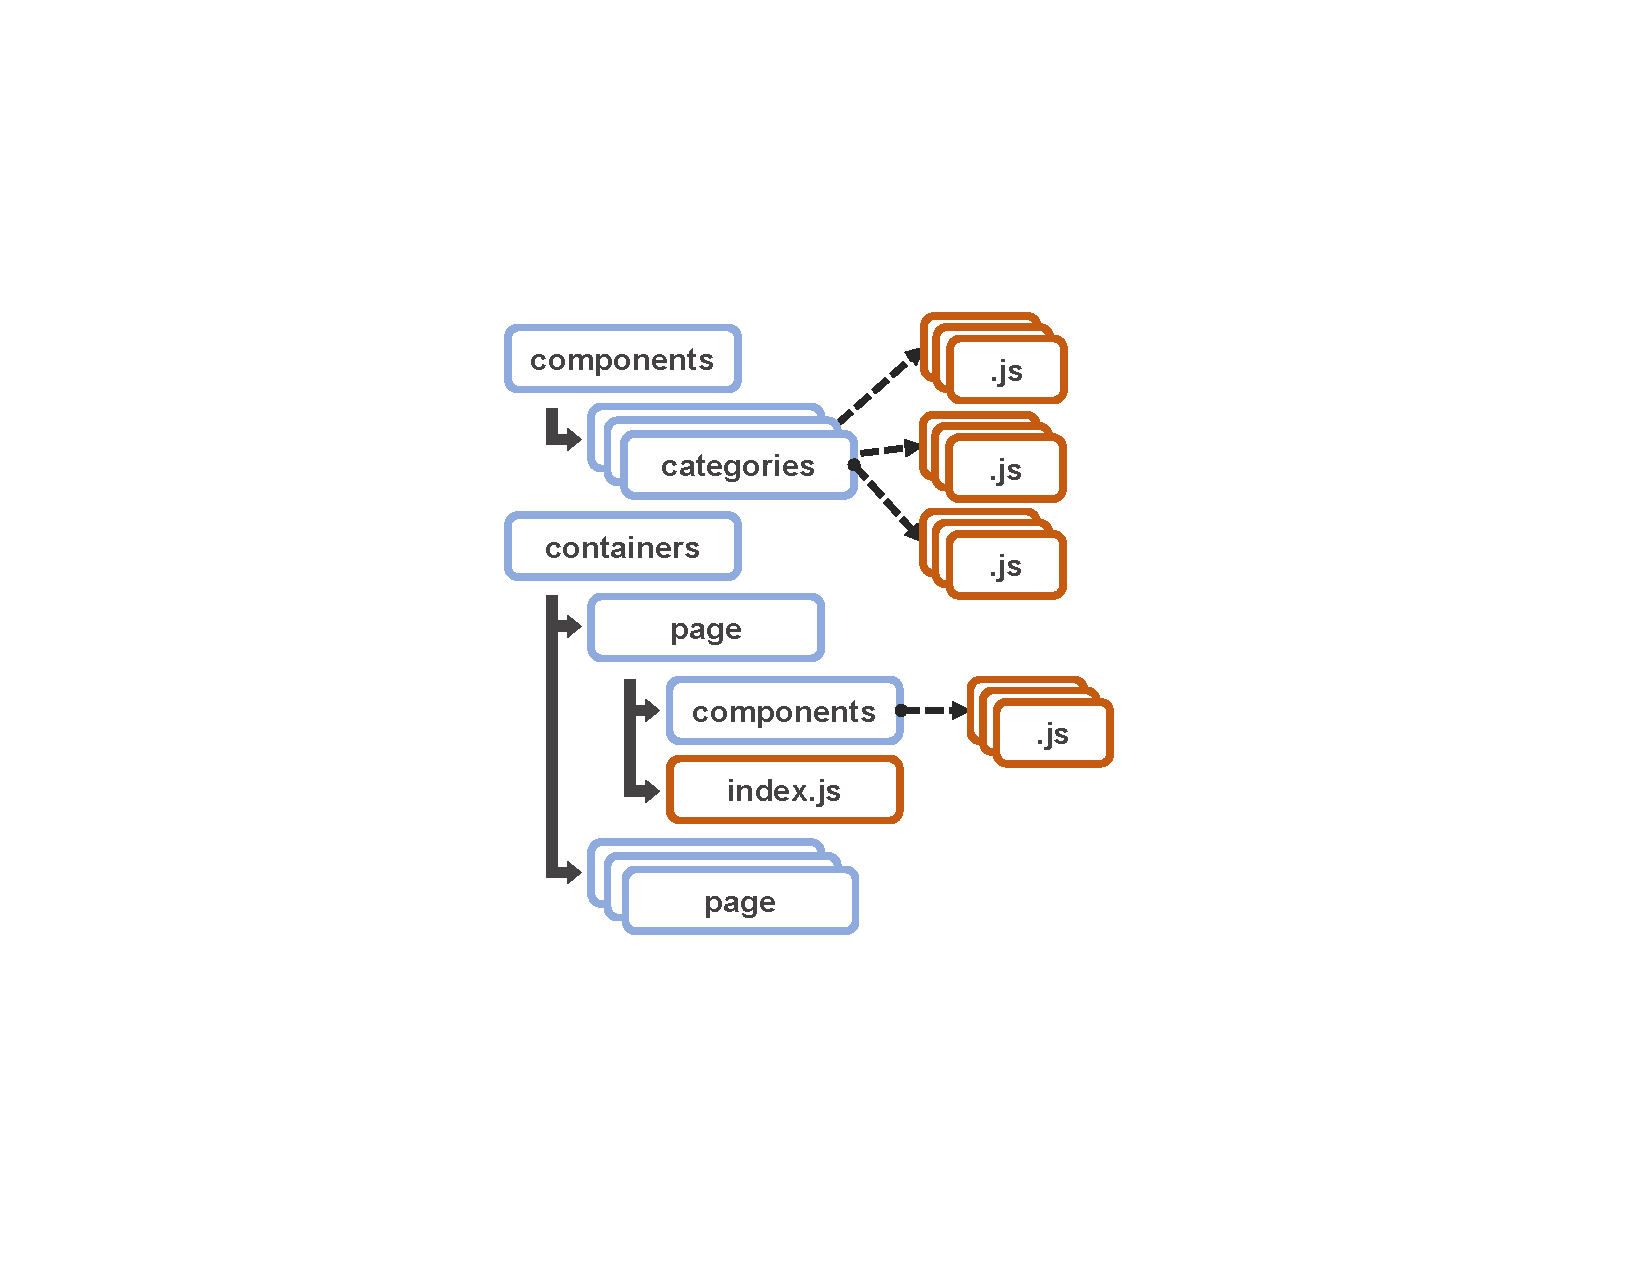
\includegraphics[scale=0.55, trim= 5cm 5cm 5cm 5cm, clip]{010architectureold}
  \caption{Basic application architecture}
  \label{fig:architectureold}
\end{figure}

The prototype was implemented keeping all best practices in mind that were explained in the Section \ref{sec:application-architecture}. In real world applications it is very complicated to entirely realize all best practices. The architecture of the prototype is also a little bit out of date as it was developed in summer 2016 and newer best practices and newer community standards have arisen until the time of this writing (May 2017).

The basic architecture of the application splits all parts into containers and components. Like mentioned before, the used application architecture is slightly out of date but it also more or less divides components into smart and dumb components. The Figure \ref{fig:architectureold} shows the prototype's current architecture. Every screen of the application has its own container section. The fact that all pages are divided into their own containers makes it easy for Webpack to codesplit the application bundle to prevent the user from having to download the complete application code if only the login screen is shown.

The biggest caveat of the current architecture is that every container still has its own specific components that are only used by that very container as the Figure \ref{fig:architectureold} tries to visualize. Application logic is scattered across multiple components which makes the whole application more difficult to understand. Oftentimes it is unclear what component of the container is connected to the store and what component handles which part of the container's logic. The solution to that problem is explained later in the Section \ref{ssec:donebetter}.

The components section of the application contains all UI elements that can be used to render simple components like a button or a text input component. As mentioned in the Chapter \ref{sec:application-architecture} the whole application should be expendable by only using existing UI components from the component library.

\subsection{Component}

As mentioned before it is very important to split the application into logical components that can be reused. A good example for a simple component would be the button component. The component wraps additional functionality around the native button DOM element that can be used throughout the whole application more comfortable and do avoid code duplication. The following example shows the basic button component of the prototype:\newline

\begin{JsCode}
/* ========================= LOAD modules =========================== */

import React, { PropTypes } from 'react'
import classNames from 'classnames'

/* ================================================================= */

const Button = (props) => {

  const className = classNames('button', props.className, {
    'button-primary': props.primary,
    'button-secondary': props.secondary,
    'button-disabled': props.disabled,
    'button-success': props.success,
    'button-failure': props.failure,
  })

  return (
    <button
      className={className}
      onClick={props.onClick}
    >
      {props.children}
    </button>
  )
}

Button.propTypes = {
  onClick: PropTypes.func.isRequired,
  className: PropTypes.string,
  primary: PropTypes.bool,
  secondary: PropTypes.bool,
  disabled: PropTypes.bool,
  success: PropTypes.bool,
  failure: PropTypes.bool,
}

export default Button
\end{JsCode}

In the prototype buttons can have multiple appearance variances. For instance, a button can be disabled or have a primary or secondary appearance. This can easily be controlled via \enquote{props} in ReactJS. In the following example the button can have many different properties that control how the button looks like. The \texttt{Button.propTypes} object shows, what properties can be set in order to change the appearance of the component. One example would be the \texttt{primary} property that transforms the button into a primary look. The \texttt{Button.propTypes} object also shows, that none of the properties is required so the button has a standard fall-back appearance if no property is set.

The property \texttt{onClick} has to be a callback function that gets executed when the button is pressed. The static \texttt{propTypes} object of the Button component has an \texttt{onClick} property that is set to \texttt{PropTypes.func.isRequired} which requires the property to be a function that must not be undefined when the component is used. Every time the button component gets clicked, React will handle the event and execute the passed callback function which has to be implemented by the user of the Button component in order to trigger some application logic.

Last but not least there is an implicit property that can be set. If a React component has children, they automatically get attached to the properties of the parent element. The children can be accessed in the parent component via \texttt{props.children}. This enables the component to process its children before embedding or rendering them. React provides a top-level API which can modify or rearrange children as it can be read in React's documentation \cite[React]{FacebookInc.2013}

\subsection{Container}

The following example shows how a standard stateful component looks like in ReactJS:\newline

\begin{JsCode}
/* ========================= LOAD modules =========================== */

import React, { Component } from 'react'
import { bindActionCreators } from 'redux'
import { connect } from 'react-redux'
import { 
  initialLoad, 
  updateFilterCriteria, 
  updateData, 
  exportData 
} from 'store/actions/data'

/* ======================= LOAD components ========================== */

import FlexContainer from 'components/common/flexContainer'
import DataTableView from './dataTableView'
import FilterCriteria from './filterCriteria'

/* ================================================================== */

const mapStateToProps = (state) => {
  return ({
    data: state.data,
    user: state.user,
  })
}

const mapDispatchToProps = (dispatch) => {
  return (
    bindActionCreators(
      {
        initialLoad,
        updateFilterCriteria,
        updateData,
        exportData,
      },
      dispatch,
    )
  )
}

class SearchDomainsPage extends Component {

  componentDidMount() {
    this.props.initialLoad()
  }

  componentWillReceiveProps(nextProps) {

    const filter = this.props.data.get('filter')
    const nextFilter = nextProps.data.get('filter')

    if (!filter.equals(nextProps.data.get('filter'))) {
      this.props.updateData(nextFilter)
    }
  }

  render() {

    // the properties are "destructured" from the this object
    // destructuring is an ES6 feature
    // the data, updateFilterCriteria and the exportData variables are extracted
    const { props: { data, updateFilterCriteria, exportData } } = this

    return (
      <div className="domain-search-page">
        <FlexContainer>
          <FilterCriteria
            updateFilterCriteria={updateFilterCriteria}
            data={data}
          />
          <DataTableView
            exportData={exportData}
            data={data}
          />
        </FlexContainer>
      </div>
    )
  }
}

export default connect(
  mapStateToProps,
  mapDispatchToProps,
)(SearchDomainsPage)
\end{JsCode}

Note how the component is connected to the Redux store of the application at the end where the component gets exported. In this advanced example the full potential of Redux is used as also the store's actions are bound to the component's properties. This feature was not described in this thesis as it would have gone beyond the scope. To learn about \texttt{react-redux}'s full potential the documentation can be read \footnote{https://github.com/reactjs/react-redux}.

The \texttt{componentWillReceiveProps} method is implemented which can react to the passed props of this component. If there was an update in the advertisement filter that queries the elastic search cluster the component will update itself via the provided callback function \texttt{updateData()} that has to be passed as prop to the component.

Because this component is a stateful component it provides the data from the store to all of its child components that are mostly dumb or stateless components in this case.

% \subsection{Important code examples}

% show some interesting code examples
% should component update
% smart dumb components
% handling state
% redux examples

\subsection{User interface explanation and demo}

The basic screen in Figure (\ref{fig:julep002}) shows the basic user interface. Some search criteria has already been applied and a list of domains and its corresponding relevant data is displayed. The list is sorted by the number of advertisement requests each domain gets. The panel \enquote{search criteria} can be used to refine the search parameters to enable more granular searches of the database. All results can also be exported as CSV files by clicking the \enquote{EXPORT} button in the top right corner of the results panel.\newline

\begin{figure}[H]
  \centering
  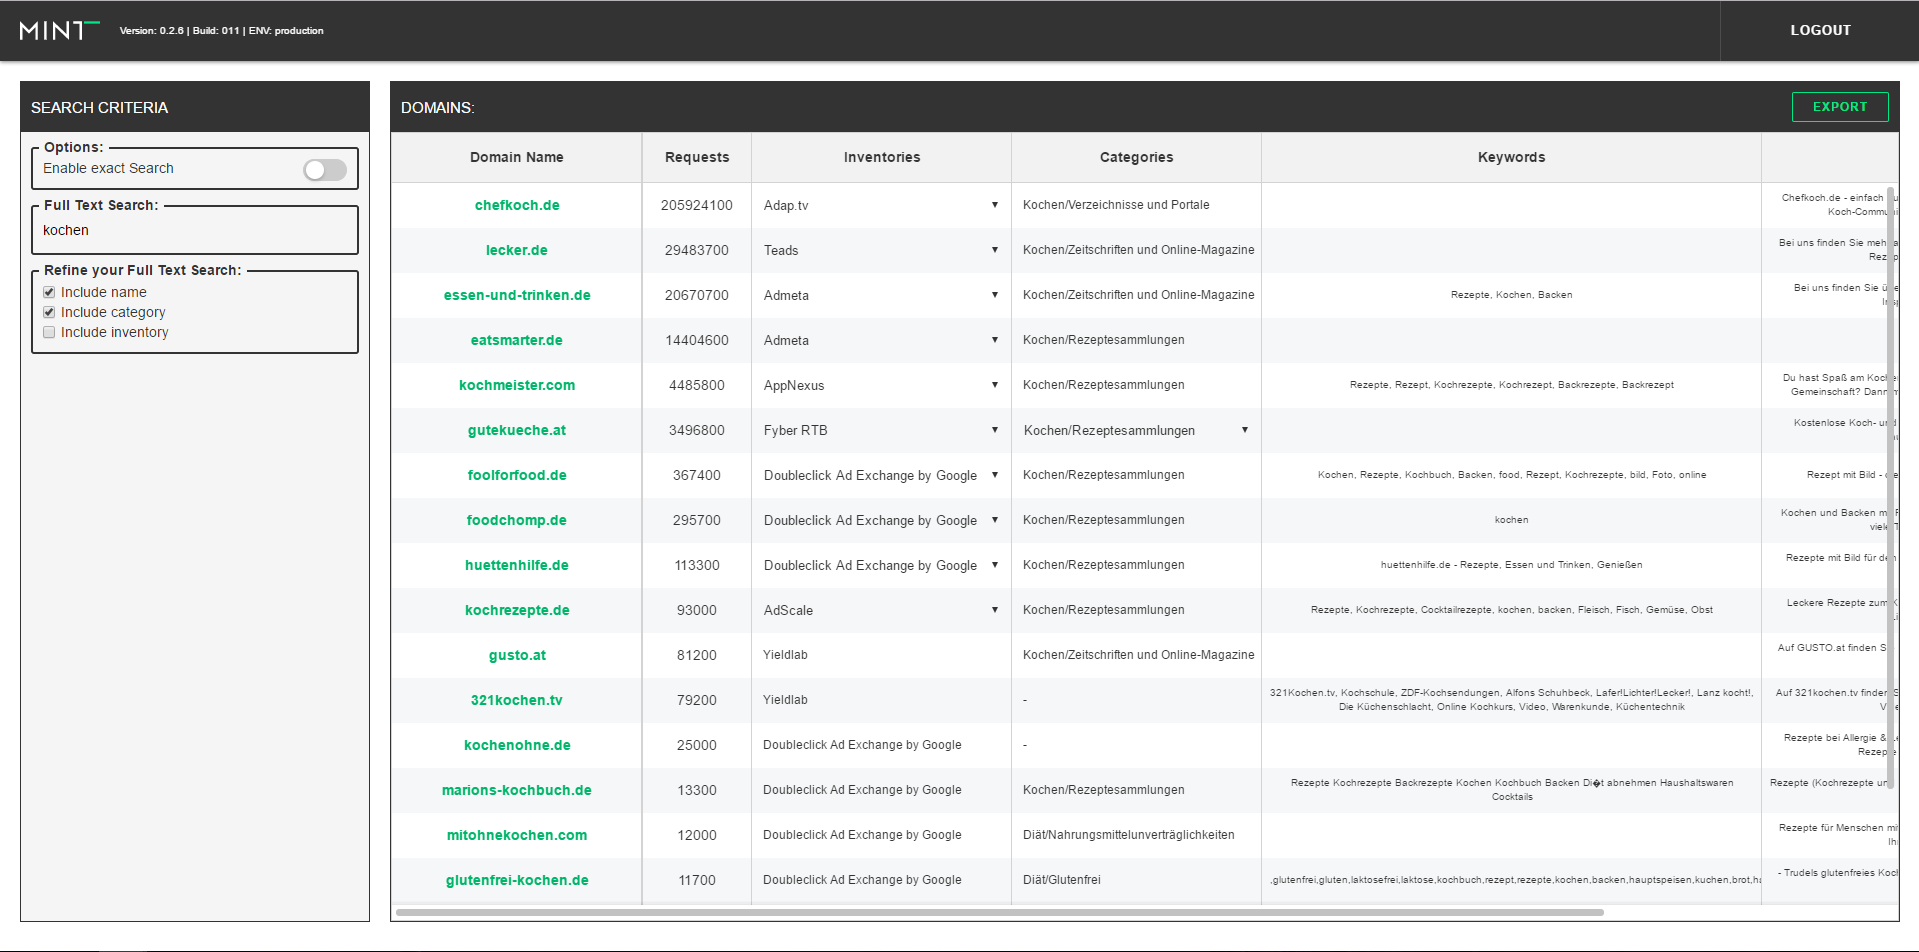
\includegraphics[width=15cm]{julep002}
  \caption{Applied search criteria in normal search}
  \label{fig:julep002}
\end{figure}

The following screen in Figure \ref{fig:julep003} shows a mockup of how the exact search could look like. As this is only a prototype the functionality was not fully implemented yet as there was no immediate demand for the feature.\newline

\begin{figure}[H]
  \centering
  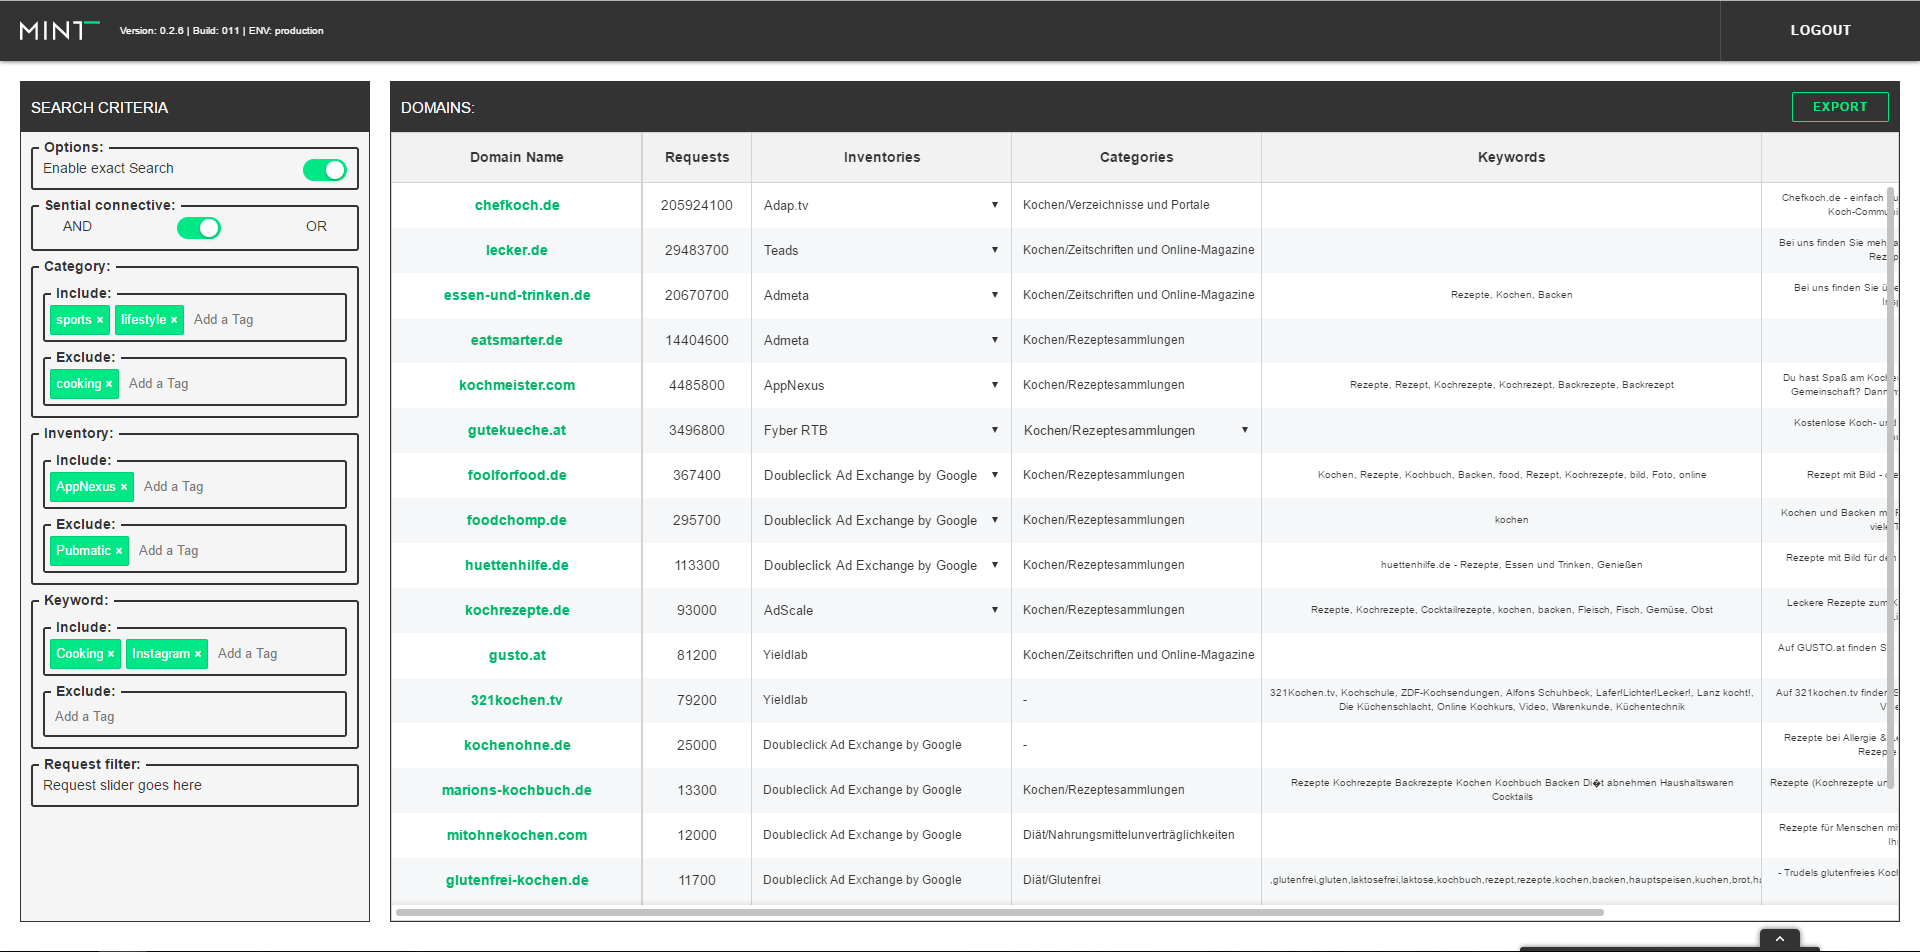
\includegraphics[width=15cm]{julep003}
  \caption{How the exact search could look like, only UI is implemented}
  \label{fig:julep003}
\end{figure}

To get a better overview over the search criteria panel, the following Figure \ref{fig:julep004} provides a better overview of the two different panels. On the left there is the basic search and on the right there is the basic implementation of the exact search panel, that does not have any logic attached to it yet.\newline

\begin{figure}[H]
  \centering
  \subfigure[normal search]{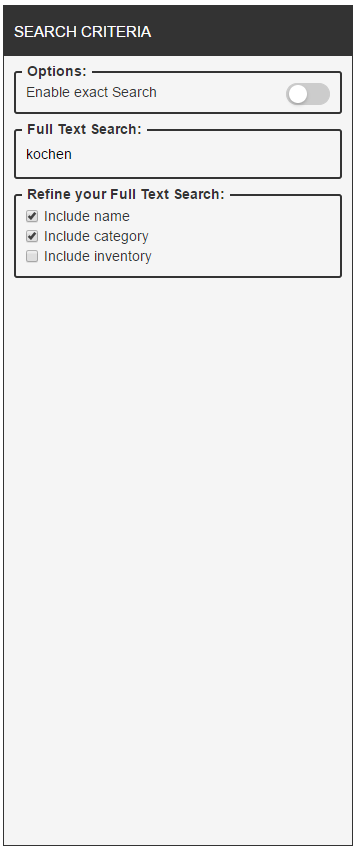
\includegraphics[height=14cm]{julep005} \label{fig:Raumeigner}} 
  \hspace{3cm}
  \subfigure[exact search]{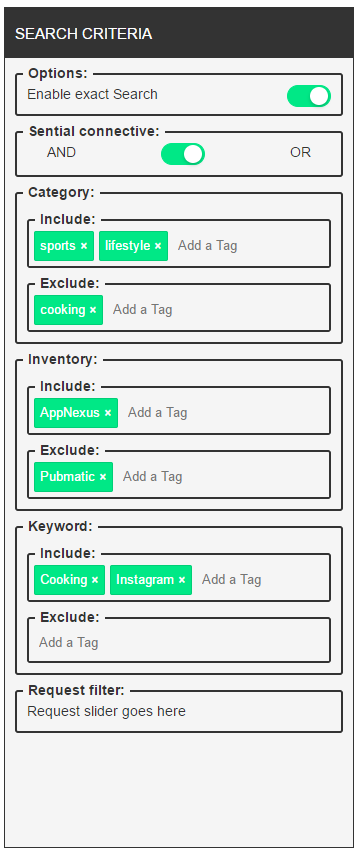
\includegraphics[height=14cm]{julep004} \label{fig:Raumverfügbar}} 
  \caption{Normal and exact search view} 
  \label{fig:julep004}
\end{figure} 

\subsection{What could have been done better} \label{ssec:donebetter}

\begin{figure}
  \centering
  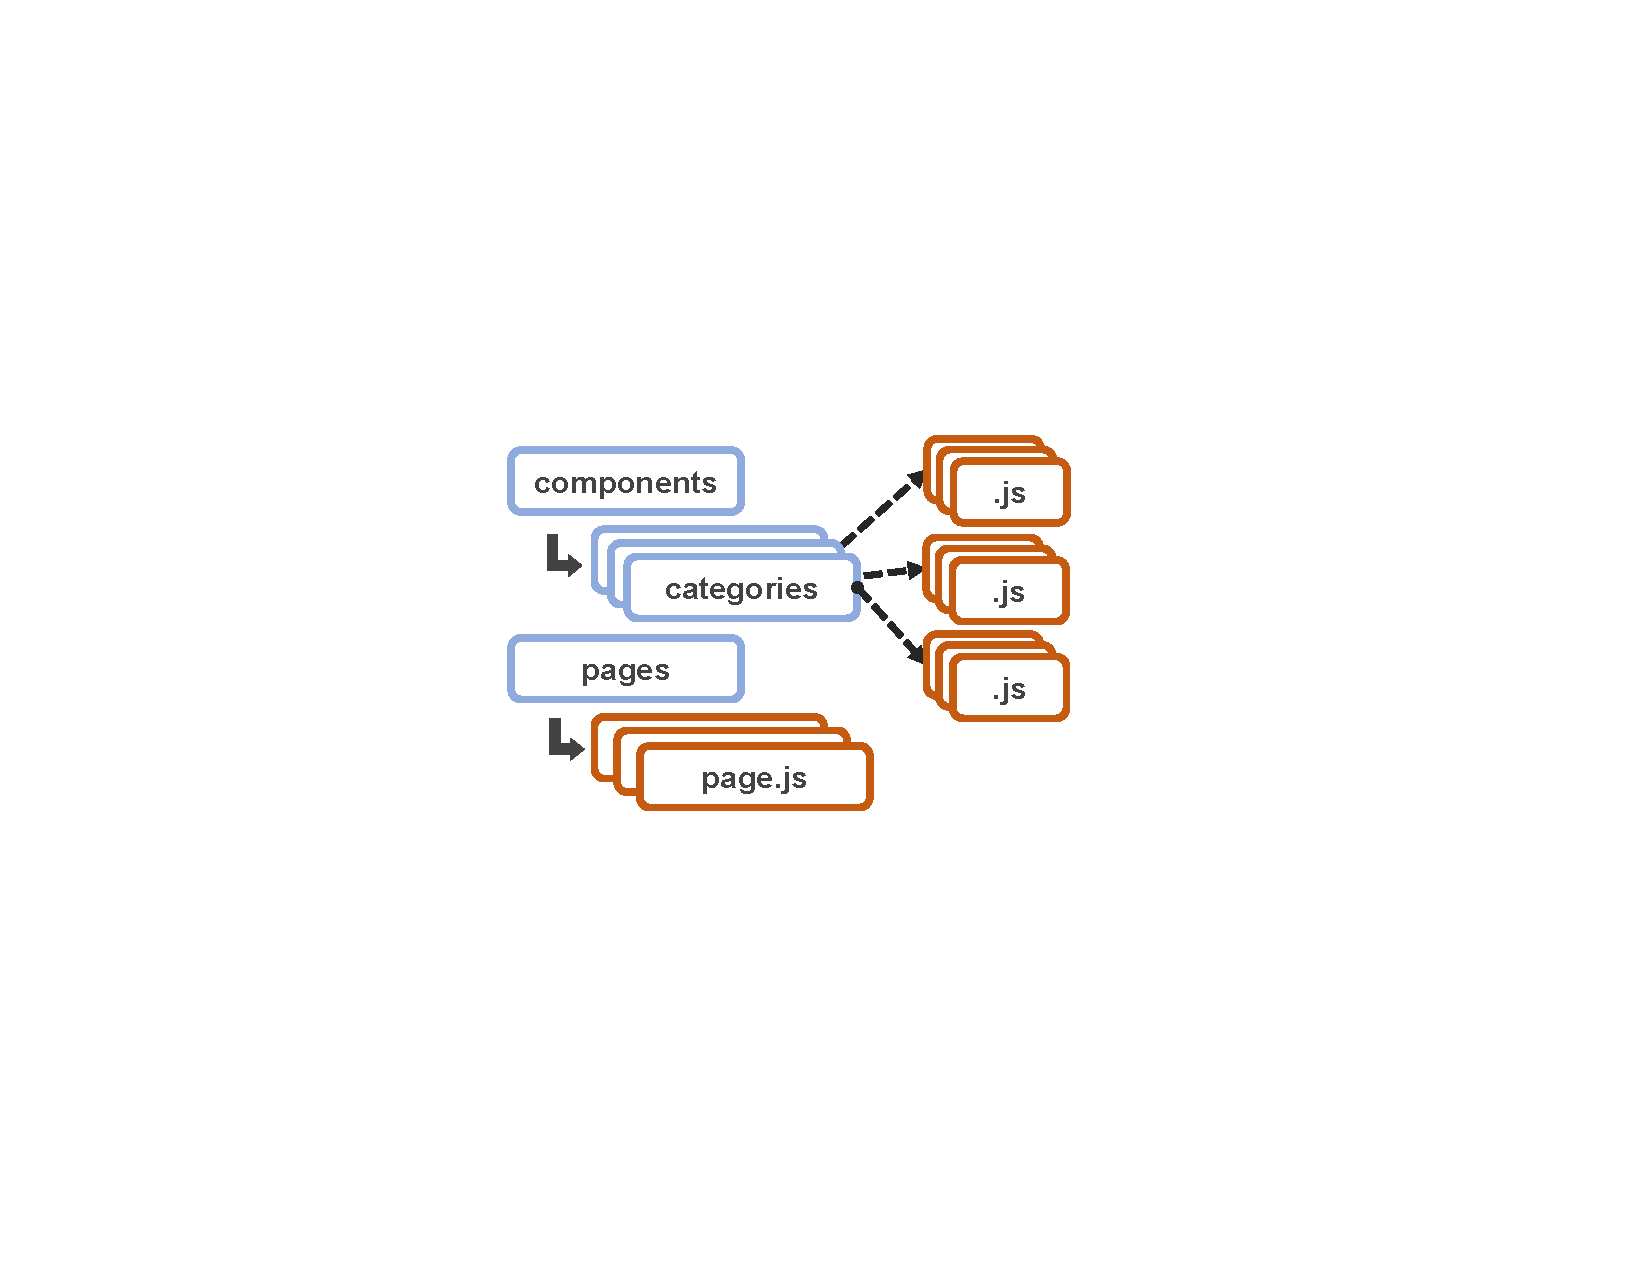
\includegraphics[scale=0.6, trim=5cm 7cm 5cm 7cm, clip]{011architecturenew}
  \caption{Better application architecture}
  \label{fig:architecturenew}
\end{figure}

In 2017 a new community standard arose that describes how to structure ReactJS applications as the Figure \ref{fig:architecturenew} shows. The whole application is divided into pages that can only use components from the component library. This should encourage developers even more to handle state and state-related logic only in one component (being the page component in this case) and pass all necessary logic down to the child components. This ensures that application-relevant logic is only handled in page components making the application much more easy to understand and to maintain.

As stated in the Section \ref{ssec:protarchitecture}, the prototype uses the slightly outdated application architecture that can be seen in the Figure \ref{fig:architectureold} that makes it noticeably more difficult to quickly understand the whole application logic. As the project is not maintained anymore the application was not refactored. The finding that the newer version of the application architecture can alleviate maintenance problems has to be kept in mind during the development of future projects.

% state what could have been done better, where errors have been made

% \subsection{There is still room for improvements}

% how could this application be improved? what is the future of this application?
% community -> page and components
% only connect page components to the store





\chapter{Conclusion}
\label{cha:conclusion}

This chapter is a recapitulation of all topics and discussions that were presented in this thesis. It is a conclusion of all findings that were discovered during the development of the prototype and the research phase of this paper.

\section{Results}

The thesis yields very interesting results that can be taken into consideration when having to decide which technology to utilize to start a web application software project. The comparison between Flux and MVC shows that flux is rather similar to MVC but also demonstrates that Flux is still a viable web application architecture. The thesis also gives an overview to web application development with ReactJS in general. It shows what effort it takes to start developing a web application with ReactJS and how the framework can be used to implement real world web applications. Finally, the paper concludes all findings by presenting a prototype that tries to incorporate all results and best practices that are presented in this thesis.

\subsection{Flux and MVC}

In conclusion Chapter \ref{cha:fluxreduxmvc} shows that Flux and MVC are very similar. Facebook introduced the Flux pattern as a brand new programming pattern but it turns out to be a copy of a slightly changed MVC pattern. Though it must be emphasized that Flux is indeed different to MVC as data is injected actively into the components, whereas MVC depends on data bindings to react to updated data.

There are many versions and mutations of the MVC pattern. In this thesis Flux is compared to the traditional version of MVC as it was developed in 1970 by the lisp community. It must be noted that there are many subversions of MVC that are even more similar to the Flux application architecture. The research of every possible MVC sub-pattern would have gone beyond the scope of this paper.

Even though Flux is very similar to MVC the pattern is still highly usable for developing web applications. The new pattern seems to be specially tailored to be used in conjunction with the ReactJS framework which indeed works very well. Using Flux and ReactJS results in well structured web applications that can be debugged and scaled rather easily as the thesis shows.

\subsection{Web application development with ReactJS}

As discussed in the Section \ref{ssec:jsx}, ReactJS is a very promising framework as it puts an abstraction layer to the view and lets programmers build user interfaces without having to know how the user interface elements are actually created in the background. This feature enables the framework to be used across all platforms. By mastering the declarative syntax of ReactJS the programmer is enabled to reuse components across all platforms including native mobile platforms.

The thesis also shows that ReactJS can be used to develop highly performance optimized web applications. By using all provided best practices it should ease the effort of the reader to develop a well structured, well scaling web application with ReactJS.

There thesis puts a strong emphasis on the importance of having a well thought-through application architecture. In fact, application architecture is important for all kinds of software projects but the thesis should have shown that it is also a very important aspect of web applications. As stated many times throughout this thesis, the application architecture aspect oftentimes gets omitted in web projects which is a big problem the web community currently has to deal with. This thesis tries to alleviate the problem by showing the reader that application architecture is an utterly important aspect of web development. 

\subsection{Prototype}

The Chapter \ref{cha:prototypejulepsearch} shows how ReactJS can be used in a real world scenario. The basic architecture is explained to provide a better overview to the prototype. Its motivation and the goals show that ReactJS can be used for all kinds of application scenarios. As stated in the Section \ref{sec:whyreactjs} and \ref{ssec:usedtechnologies} the prototype also shows that Facebook's framework does not make many assumptions about the development stack and can be used in conjunction with many different web technologies.

As time progresses the whole ReactJS ecosystem is evolving. Since the time of developing the prototype certain best practices were omitted and others were added. In addition to a constantly changing ecosystem the lack of experience of how to develop a well structured ReactJS application complicated the development of the prototype. The last Section \ref{ssec:donebetter} shows what could have been done better.





%%%----------------------------------------------------------
\appendix                                            % Anhang 
%%%----------------------------------------------------------

%\chapter{Technische Informationen}
\label{ch:TechnischeInfos}

\newcommand*{\checkbox}{{\fboxsep 1pt%
\framebox[1.30\height]{\vphantom{M}\checkmark}}}

\section{Aktuelle Dateiversionen}

\begin{center}
\begin{tabular}{|l|l|}
\hline
Datum & Datei \\
\hline\hline
\hgbthesisDate & \texttt{hgbthesis.cls} \\
\hline
\hgbDate       & \texttt{hgb.sty} \\
\hline
\end{tabular}
\end{center}




\section{Details zur aktuellen Version}


Das ist eine völlig überarbeitete Version der DA/BA-Vorlage, die
\mbox{UTF-8} kodierten Dateien vorsieht und ausschließlich im PDF-Modus arbeitet.
Der "`klassische"' DVI-PS-PDF-Modus wird somit nicht mehr unterstützt! 

\subsection{Allgemeine technische Voraussetzungen}

Eine aktuelle \latex-Installation mit
\begin{itemize}
	
		\item Texteditor für \mbox{UTF-8} kodierte (Unicode) Dateien,
		\item \texttt{biber}-Programm (BibTeX-Ersatz, Version $\geq 1.5$),
		\item \texttt{biblatex}-Paket (Version $\geq 2.5$, 2013/01/10),
		\item Latin Modern Schriften (Paket \texttt{lmodern}).%
			\footnote{\url{http://www.ctan.org/pkg/lm}, \url{http://www.tug.dk/FontCatalogue/lmodern}}
\end{itemize}


\subsection{Verwendung unter Windows}

Eine typische Installation unter Windows sieht folgendermaßen aus
(s.\ auch Abschnitt \ref{sec:Windows}):
%
\begin{enumerate}
\item \textbf{MikTeX 2.9}%
	\footnote{\url{http://www.miktex.org/} -- \textbf{Achtung:} 
	Generell wird die \textbf{Komplett\-installation} von MikTeX ("`Complete MiKTeX"') empfohlen, 
	da diese bereits alle notwendigen Zusatzpakete und Schriftdateien enthält! 
	Bei der Installation ist darauf zu achten, 
	dass die automatische Installation erforderlicher Packages 
	durch "`\emph{Install missing packages on-the-fly: = Yes}"' ermöglicht wird (NICHT "`\emph{Ask me first}"')!
	Außerdem ist zu empfehlen, unmittelbar nach der Installation von MikTeX mit dem Programm
	\texttt{MikTeX} $\to$ \texttt{Maintenance} $\to$ \texttt{Update} und \texttt{Package Manager} 
	ein Update der installierten Pakete durchzuführen.}
	(zurzeit am einfachsten die 32-Bit Version, da nur diese das Programm \texttt{biber.exe} 
	bereits enthält),
\item \textbf{TeXnicCenter 2.0}%
	\footnote{\url{http://www.texniccenter.org/}}
	(Editor-Umgebung, unterstützt UTF-8),
\item \textbf{SumatraPDF}%
	\footnote{\url{http://blog.kowalczyk.info/software/sumatrapdf/}} 
	(PDF-Viewer),
\end{enumerate}
%
Ein passendes TeXnicCenter-Profil für MikTeX, Biber und Sumatra ist in diesem Paket enhalten
(Datei \verb!_tc_output_profile_sumatra_utf8.tco!). Dieses sollte man zuerst
über \texttt{Build} $\to$ \texttt{Define Output Profiles} in TeXnicCenter importieren.
\textbf{Achtung}: Alle neu angelegten \texttt{.tex}-Dateien sollten in UTF-8 Kodierung gespeichert werden!




\subsection{Verwendung unter Mac~OS}


Diese Version sollte insbesondere mit \emph{MacTeX} problemlos laufen (s.\ auch Abschnitt \ref{sec:MacOs}):
\begin{enumerate}
\item 
	\emph{MacTex} (2012 oder höher).
\item 
	Die Zeichenkodierung des Editors sollte auf UTF-8 eingestellt sein.
\item 
	Als Engine (vergleichbar mit den Ausgabeprofilen in TeXnicCenter) sollte \emph{LaTeXMk} verwendet werden. 
	Dieses Perl-Skript erkennt automatisch, wie viele Aufrufe von \emph{pdfLaTeX} und \emph{Biber} nötig sind. 
	Die Ausgabeprofile \emph{LaTeX} oder \emph{pdfLaTeX} hingegen müssen mehrmals aufgerufen werden, 
	zudem werden hierbei auch die Literaturdaten nicht verarbeitet. Dazu müsste extra die \emph{Biber}-Engine 
	aufgerufen werden, 	die jedoch noch nicht in allen Editoren vorhanden ist.
\end{enumerate}


\begin{comment}
\subsection{Vorteile}
\begin{itemize}
\item PDF wird direkt erzeugt ohne DVI und PS; damit ist angeblich auch die "`Feintypographie"' besser.
\item Die Verwendung von \texttt{SumatraPDF} erlaubt funktionierende Forward- und Inverse-Suche, womit erstmals ein effektiver PDF-Workflow möglich ist.
\item Preview der vollständigen Manuskripts (inklusive Grafiken) ist in PDF viel schneller
als in DVI (mit YAP und Ghostscript für die Grafiken).
\item Grafiken können auch als PDF, PNG oder JPEG direkt eingebunden werden. Bestehende EPS-Grafiken werden automatisch in PDF konvertiert. 
\item Bei eingebundenen Rasterbildern werden (im Unterschied zu \texttt{ps2pdf} in der Default-Einstellung) keine zusätzlichen JPEG-Artefakte erzeugt. 
(Anmerkung: im TC-Ausgabeprofil für \texttt{ps2pdf} ist dafür jetzt die
Option \verb!-dPDFSETTINGS=/prepress! eingestellt -- \verb!=/printer! ist nicht ausreichend!)
\item Die Erzeugung von aktiven Verweisen mit \texttt{hyperref} funktioniert problemlos, mit allen Vorteilen (einschließlich der Zeilenumbrüche in URLs).
\item PDF-Metadaten (zur verbesserten Suche) werden direkt aus den Dokumentendaten durch LaTeX generiert.
\end{itemize}

\subsection{Weitere Neuerungen}
%
\begin{sloppypar}
\begin{itemize}
\item Verwendung des \texttt{epstopdf}-Pakets, wodurch vorhandene EPS-Grafiken (mit denen \texttt{pdflatex} nicht umgehen kann) automatisch in PDF-Dateien konvertiert werden, unter der Annahme, dass \texttt{epstopdf.exe} vorhanden ist. Das ist bei Rasterbildern allerdings nicht zu enpfehlen, weil mit \texttt{epstopdf} die Kompressionsqualität nicht gesteuert erden kann. In diesem Fall ist es besser, die EPS-Dateien (\zB\ mit PhotoShop) direkt in PDFs zu konvertieren oder (noch besser) die Original JPEG- oder PNG-Dateien zu verwenden.
%
\item Unter \texttt{pdflatex} können nun (mit \verb!\includegraphics{}!) neben PDFs auch Bilder im JPEG- oder PNG-Format direkt eingebunden werden. Alle Datei-Extensions der Grafikdateien wurden im Quelltext entfernt.
%
\item 
Verwendung des \textbf{SumatraPDF}-Viewers anstelle von Adobe Acrobat, da Acrobat das Überschreiben der Ausgabedatei blockiert (unter Windows) und forward/inverse Suche schlecht \bzw\ gar nicht unterstützt.
Anweisungen zur Einstellung findet man unter \url{http://www.hehn.biz/Mar/How_to_Sumatra.pdf} -- diese sind auch im beiliegenden TC-Aus\-gabe\-profil implementiert.
%
\item Verwendung des \texttt{pdfsync}-Pakets zur Unterstützung der inversen Suche aus PDF-Dateien.
%
\item Verwendung des \texttt{hyperref}-Pakets zur Aktivierung von Links (Web, Inhaltsverzeichnis, Querverweise, Literatur etc.). Erzeugt auch eine Navigation-Pane.
%
\item PDF-Metadaten werden automatisch aus den Dokumentendaten generiert (durch \texttt{hyperref} möglich).
%
\item Verwendung des \texttt{breakurl}-Pakets, mit dem Zeilenumbrüche trotz \texttt{hy\-per\-ref} auch bei DVI-PS-PDF-Generierung durchgeführt werden. Dadurch sind jetzt auch URLs in Captions und Fußnoten problemlos möglich und auch \verb!\urldef{}! ist nicht mehr erforderlich (entspr.\ Textpassagen in \ref{sec:QuellenangabenInCaptions} entfernen!). 
%
\item Alle bestehenden EPS-Dateien mit Rasterbildern wurden auf Binärkodierung umgestellt, da dies mit der aktuellen MikTeX-Version keine Probleme mehr verursacht. Zusätzlich wurden PNG-Versionen für \texttt{pdflatex} angelegt, sodass keine automatische Umwandlung mit \texttt{epstopdf} erfolgt.
%
\item
Das lästige Problem des übermäßigen vertikalen Abstände in LaTeX-Aufzählungslisten wurde mit dem \texttt{enumitem}-Paket behoben. Alle \verb!\itemsep0pt! Anweisungen im Text wurden entfernt.
%
\item Einbindung des \texttt{cite}-Pakets mit \texttt{noadjust}-Option, womit kein zusätzliches Spacing erzeugt wird.
\end{itemize}
\end{sloppypar}
\end{comment}


\begin{comment}
\section{Einstellungen unter Windows} 
\label{sec:EinstellungAusgabeprofile}

Die folgenden Angaben beziehen sich auf eine bewährte Arbeitsumgebung unter Windows (XP, Win7) mit MikTeX, Sumatra-PDF und TeXnicCenter, mit folgenden Installationspfaden:
%
\begin{quote}
\verb!C:\Program Files (x86)\MiKTeX 2.9\! \\
\verb!C:\Program Files (x86)\SumatraPDF\! \\
\verb!C:\Program Files (x86)\TeXnicCenter\! 
\end{quote}
%
Unter Windows XP liegen die Programme in \verb!C:\Program Files\!.
Falls neuere Versionen dieser Komponenten installiert sind, müssen natürlich die nachfolgend angegebenen Pfade entsprechend modifiziert werden.

\begin{quote}
\textbf{Achtung:} Für MikTeX immer die \textbf{komplette Version} installieren! Das entsprechende Installationsverzeichnis hat aktuell einen Umfang von ca.\ 1.2 GB und enthält etwa 53.200 Dateien 
(typischerweise in \nolinkurl{C:\\Program Files (x86)\\MiKTeX...}).
\end{quote}
\end{comment}

\begin{comment}
\subsection{TeXnicCenter-Ausgabeprofile}
\label{sec:TeXnicCenterUndMikTeX}

TeXnicCenter definiert den Verarbeitungsablauf des LaTeX-Dokuments anhand von Ausgabeprofilen, wobei die oben genannten Komponenten als externe Programme mit entsprechenden Argumenten aufgerufen werden.
Die Einstellung der Ausgabeprofile erfolgt in TeXnicCenter über das Menü
\textsf{Ausgabe}$\rightarrow$\textsf{Ausgabeprofile definieren...} (Abb.\ \ref{fig:techniccenter-profile-latex}). 
Die Profile werden (abhängig von der installierten Software) üblicherweise beim ersten Start von TeXnicCenter durch den zugehörigen "`Wizard"' voreingestellt. 

\begin{figure}
\centering\small
\setlength{\tabcolsep}{0pt}%
\begin{tabular}{c@{~}c}
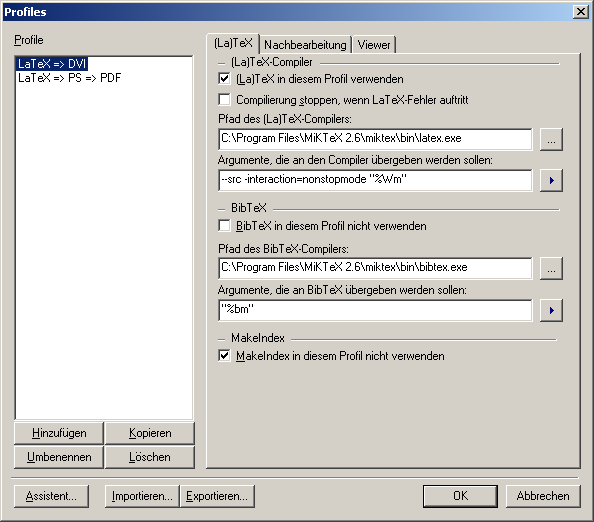
\includegraphics[width=0.49\textwidth]{techniccenter-profile-dvi-26} &
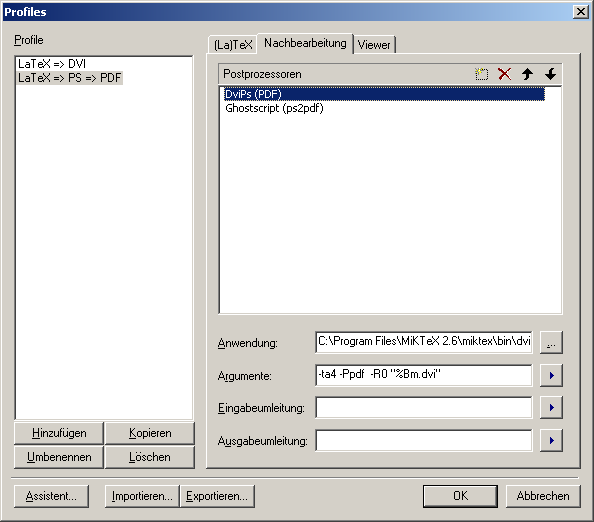
\includegraphics[width=0.49\textwidth]{techniccenter-profile-dvips-26} \\[4pt]
(a) & (b)
\end{tabular}
\caption{Spezifikation der Ausgabeprofile in TeXnicCenter.}
\label{fig:techniccenter-profile-latex}
\end{figure}

In der Datei \verb!tc_output_profiles_sumatra.tco! sind  folgende beiden "`maßgeschneiderten"' Ausgabeprofile für TexNicCenter angelegt (Import über \textsf{Build} $\rightarrow$ \textsf{Define Output Profiles ...}):
\begin{itemize}
	\item \verb!LaTeX => PDF (Sumatra)! -- Standard, direkte Erzeugung von PDF,
	\item \verb!LaTeX => PS => PDF (Sumatra)! -- PDF "`klassisch"' via DVI und PS.
\end{itemize}

\subsubsection{Profil "`\texttt{LaTeX => PDF (Sumatra)}"'}

Das ist das mit diesem Setup normalerweise verwendete Standardprofil.

\paragraph{(La)Tex:}
\begin{itemize}
  \item Path to the (La)TeX compiler: \\
        \begin{small} \verb!C:\Program Files (x86)\MiKTeX 2.9\miktex\bin\pdflatex.exe!\end{small}
  \item Command line arguments to pass to the compiler:\\
\begin{small}
   \verb!-synctex=-1 -interaction=nonstopmode "%pm"!
\end{small}
\end{itemize}

\paragraph{Postprocessor:} 
leer, kein Postprocessor notwendig.

\paragraph{Viewer:}
\begin{itemize}
\item Path of executable: \\
\begin{small}
    \verb!C:\Program Files (x86)\SumatraPDF\SumatraPDF.exe ! \\ 
    \verb!-inverse-search "\"C:\Program Files\TeXnicCenter\TEXCNTR.EXE\" !\\
    \verb!/ddecmd \"[goto('%f','%l')]\""!
\end{small}
%
\item View project's output: \\
\begin{small}
    \checkbox\ Command line argument \\\
    Command: \verb!"%bm.pdf"!
\end{small}
%
\item Forward search:\\
\begin{small}
    \checkbox\ DDE command \\\
    Command: \verb![ForwardSearch("%bm.pdf","%Wc",%l,0)]! \\
    Server: \verb!SUMATRA! \\
    Topic: \verb!Control!
\end{small}
\item Close document before running (La)TeX:\\
\begin{small}
    \checkbox\ Do not close
\end{small}
\end{itemize}


\subsubsection{Profil "`\texttt{LaTeX => PS => PDF (Sumatra)}"'}

Profil ausschließlich für den DVI-PS-Workflow (über DVI und PostScript).

\paragraph{(La)Tex:}
\begin{itemize}
  \item Path to the (La)TeX compiler: \\
        \begin{small} \verb!C:\Program Files (x86)\MiKTeX 2.9\miktex\bin\latex.exe!\end{small}
  \item Command line arguments to pass to the compiler:\\
\begin{small}
   \verb!-synctex=-1 -interaction=nonstopmode "%pm"!
\end{small}
\end{itemize}

\paragraph{Postprocessor:}
\begin{itemize}
  \item DviPS (PDF): \\
        \begin{small} 
        Executable: \verb!C:\Program Files (x86)\MiKTeX 2.9\miktex\bin\dvips.exe! \\
        Arguments: \verb!-ta4 -P pdf -R0 "%Bm.dvi"!
        \end{small}
  \item Ghostscript (ps2pdf):\\
  		\begin{small} 
        Executable: \verb!C:\Program Files (x86)\gs\gs9.04\bin\gswin32c.exe! \\
        Arguments: \verb!-q -dPDFSETTINGS=/prepress -sPAPERSIZE=a4 -dSAFER! \\
         \verb!-dBATCH -dNOPAUSE -sDEVICE=pdfwrite -sOutputFile="%bm.pdf"! \\
         \verb!-c save pop -f "%bm.ps"!
      \end{small}
\end{itemize}

\paragraph{Viewer:}
wie in Profil A. (\texttt{LaTeX => PDF (Sumatra)}).

\section{Tipps und offene Probleme:}

\begin{itemize}
\item \texttt{psfrag} funktioniert nicht mit \texttt{pdflatex} und es gibt auch leider keine Ersatzlösung. 
Wenn man \texttt{psfrag} braucht, dann muss man weiterhin über PostScript 
(\verb!LaTeX => PS => PDF!) arbeiten (was allerdings nunmehr auch mit \texttt{hyperref} kein Problem mehr ist).
%
\item Bei Verwendung des TexWorks-Editors (wird mit MikTeX ausgeliefert) sollte man die Standard-Zeichenkodierung von \emph{Unicode} (utf8) auf \emph{Latin-1} (ISO 8859-1) umstellen.
%
\item Adobe Illustrator kann beim Speichern als PDF die Bounding Box nicht setzen. 
Eine Möglichkeit ist, die Grafik zuerst als EPS zu exportieren und dann mit Acrobat in ein PDF zu konvertieren. 
%
\end{itemize}
\end{comment}



\begin{comment}
\section{Einstellungen für YAP (DVI-Viewer) im DVI-PS-Workflow}
\label{sec:YapEinstellung}

Im Standard-DVI-Viewer YAP lässt sich durch Mausklick auf das DVI-Dokument sehr leicht die zugehörige Stelle im Quelltext finden. Im Normalfall öffnet dann TeXnicCenter das zugehörige \latex-Dokument automatisch an der richtigen Stelle.
Das zugehörige "`Inverse DVI Search"' Kommando sollte sich bereits bei der Installation richtig einstellen.

Falls dies \emph{nicht} funktioniert, kann man in YAP diese Einstellung auch manuell über das Menü \textsf{View}\thinspace$\rightarrow$\thinspace\textsf{Options...} vornehmen, wie in Abb.\ \ref{fig:yap-inverse-search} gezeigt.
In diesem Fall lautet die vollständige Anweisung in "`Command Line"' folgendermaßen:
\begin{center}\footnotesize
\verb!"C:\Program Files (x86)\TeXnicCenter\TEXCNTR.EXE" /ddecmd "[goto('%f', '%l')]"!
\end{center}


\begin{figure}
\centering\small
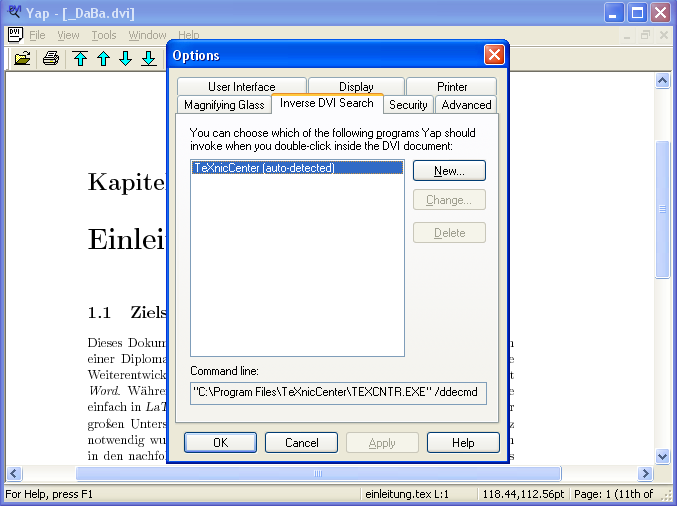
\includegraphics[width=1.0\textwidth]{yap-inverse-search-settings}
\caption{"`Inverse DVI Search"' Einstellung in YAP (über das Menü \textsf{View}\thinspace$\rightarrow$\thinspace\textsf{Options...}).}
\label{fig:yap-inverse-search}
\end{figure}

Latex
C:\Program Files\MiKTeX 2.6\miktex\bin\latex.exe
--src -interaction=nonstopmode "%Wm"

Bibtex
C:\Program Files\MiKTeX 2.6\miktex\bin\bibtex.exe
"%bm"

---

DviPs (PDF)
C:\Program Files\MiKTeX 2.6\miktex\bin\dvips.exe
-ta4 -Ppdf  -R0 "%Bm.dvi"

Ghostscript (ps2pdf)
C:\Program Files\gs\gs8.61\bin\gswin32c.exe
-sPAPERSIZE=a4 -dSAFER -dBATCH -dNOPAUSE -sDEVICE=pdfwrite -dPDFSETTINGS=/prepress -sOutputFile="%bm.pdf" -c save pop -f "%bm.ps"


YAP 
Options -> Inverse Search
"C:\Program Files\TeXnicCenter\TEXCNTR.EXE" /ddecmd "[goto('%f', '%l')]"

\end{comment}

	% Technische Ergänzungen
%\chapter{Inhalt der CD-ROM/DVD}
\label{app:cdrom}

\paragraph{Format:} 
		CD-ROM, Single Layer, ISO9660-Format%
\footnote{Verwenden Sie möglichst ein Standardformat, bei DVDs natürlich
eine entsprechende andere Spezifikation.}


\section{PDF-Dateien}
\begin{FileList}{/}
%\fitem{_DaBa.dvi} Gesamtdokument (DVI-File, ohne Grafiken)
\fitem{_DaBa.pdf} Master- oder Bachelorarbeit mit Instruktionen (Gesamtdokument)
\fitem{_PrBericht.pdf} Praktikumsbericht (verkürzte Version der Bachelorarbeit) %
\end{FileList}


\section{\latex-Dateien}

\textbf{Achtung:} Die folgende Auflistung soll nur den Gebrauch dieser Vorlage erleichtern. Es ist bei einer Master- oder Bachelorarbeit \ia\ \emph{nicht} notwendig, die zugehörigen \latex-Dateien aufzulisten (wohl aber projektbezogene Dateien, Ergebnisse, Bilder, Kopien von Online-Literatur etc.)!

\begin{FileList}{/}
\fitem{_DaBa.tex} Master-/Bachelorarbeit (Hauptdokument) %
\fitem{_PrBericht.tex} Praktikumsbericht (verkürzte Version der Bachelorarbeit) %
\fitem{vorwort.tex} Vorwort %
\fitem{kurzfassung.tex} Kurzfassung %
\fitem{abstract.tex} Abstract %
\fitem{einleitung.tex} Kapitel 1 %
\fitem{diplomschrift.tex} Kapitel 2 %
\fitem{latex.tex} Kapitel 3
\fitem{abbildungen.tex} Kapitel 4 %
\fitem{formeln.tex} Kapitel 5 %
\fitem{literatur.tex} Kapitel 6 %
\fitem{drucken.tex} Kapitel 7 %
\fitem{word.tex} Kapitel 8 %
\fitem{schluss.tex} Kapitel 9 %
\fitem{anhang_a.tex} Anhang A (Source Code) %
\fitem{anhang_b.tex} Anhang B (Inhalt CD-ROM) %
\fitem{anhang_c.tex} Anhang C (Liste der Änderungen) %
\fitem{anhang_d.tex} Anhang D (LaTeX-Quellcode) %
\fitem{messbox.tex} Messbox zur Druckkontrolle %
\fitem{literatur.bib} Literatur-Datenbank (BibTeX-File)
\end{FileList}

\section{Style/Class-Dateien}

\begin{FileList}{/}
\fitem{hgbthesis.cls} LaTeX Class-Datei für Master- und Bachelorarbeiten
\fitem{hgbtermreport.cls} LaTeX Class-Datei für Semesterberichte
\fitem{hgb.sty} LaTeX Style-Datei für alle Hagenberg-Dokumente
\end{FileList}


\section{Sonstiges}

\begin{FileList}{/images}
\fitem{*.ai} Original Adobe Illustrator-Dateien %
\fitem{*.fh11} Original Macromedia Freehand-Dateien %
\fitem{*.jpg, *.png} Original Rasterbilder %
%\fitem{*.eps} Bilder und Grafiken im EPS-Format%
%\fitem{fonts-bakoma/} BaKoMa TrueType Fonts %
\end{FileList}
	% Inhalt der CD-ROM/DVD
%\chapter{Chronologische Liste der Änderungen}


\begin{sloppypar}
\begin{description}
%
\item[2002/01/07]
\verb!\newfloat{program}! repariert (auch ohne Chapter). Dank an Werner Bailer!
%
\item[2002/03/06]
Copyright-Notice an internat.\ Standard angepasst. Dank an Karin Kosina!
%
\item[2002/07/28]
"`Studiengang"' $\rightarrow$ "`Diplomstudiengang"'
%
\item[2003/08/24]
Neues Macro: \verb!\Messbox{breite}{hoehe}! -- zur Kontrolle der 
Druckgröße ohne PS-Datei. Erweiterungen für Bakkalaureatsarbeiten
%
\item[2005/04/09]
Diverse Korrekturen: Captions von Tabellen nach oben gesetzt. 
\texttt{caption} auf neue Versionen adaptiert.
\texttt{subfigure} wird nicht mehr verwendet
%
\item[2006/01/20]
Adaptiert zur Verwendung als Praktikumsbericht 
(2.\ Bakk.-Arbeit)
%
\item[2006/03/24]
Fehler in \verb!\erklaerung! beseitigt (Dank an David Schwingenschlögl)
%
\item[2006/04/06]
Verwendung von T1-Fontencoding zur besseren Silbentrennung bei 
Umlauten etc.
%
\item[2006/06/21]
Neu: Bachelorstudiengang / Masterstudiengang.
Literaturverweise auf Bakk-Arbeiten.
\texttt{upquote.sty} eliminiert (Problem mit TS1-Kodierung).
Verwende Komma (statt Punkt) als Trennzeichen in Dezimalzahlen.
%
\item[2006/09/14]
Anmerkungen zum Thema Plagiarismus.
%
\item[2007/07/16]
Ergänzungen für Code-Listings (listings) und Algorithmen 
(\texttt{algorithmicx}).
BiBTeX-Datei aufgeräumt, Verwendung der Literaturformate 
verbessert.
Komma (statt Punkt) als Trennzeichen in Dezimalzahlen wieder 
entfernt.
Verwendung der \texttt{ae}-Fonts eliminiert (\texttt{cm-super} Fonts müssen 
installiert sein, ab MikTeX 2.5). 
Beispiel für Ersetzung in EPS-Dateien mit \texttt{psfrag}.
%
\item[2007/10/04]
Version 5.90: Das Laden der Pakete \verb!inputenc! (Option \texttt{latin}) und 
\verb!graphicx! (Option \texttt{dvips})
aus der Hauptdatei in die \texttt{sty}-Datei übertragen; \texttt{upquote} funktioniert nun.
Paket \texttt{eurosym} ergänzt für Euro-Symbol (Anregung von Andreas 
Doubrava).
Problem mit \texttt{color}-package repariert (gerasterter PDF-Ausdruck).
Hinweise bzgl.\ Literatur ergänzt (\texttt{month}, \texttt{edition}),
BibTeX-Datei gesäubert.
Hinweis zum Einfügen von vertikalem Abstand zwischen Absätzen.
Mathematik aufgeräumt, Verwendung von \texttt{amsmath}, 
Fallunterscheidungen.
Diverse Änderungen bei Tabellen und Programmkode.
Beispiele für BibTeX-Angaben von Spezialquellen: Audio-CDs, 
Videos, Filme. Einbinden von Dateien mit \verb!\include{..}!
Neue Datei: \verb!_SimpleReport.tex! für kurze Reports (Projekte etc.).
%
\item[2007/11/11]
Version 5.91: Hinweise zur Einstellung der Output-Profile in
TexNicCenter, Inverse Search Einstellung in YAP im Anhang.
%
\item[2008/04/01]
Version 6.00beta -- kompletter Umbau!
Auslagerung der Doku\-menten-relevanten Teile in eine eigene 
\emph{class}-Datei (\texttt{hgbthesis.cls}) mit Optionen.
Die neue Style-Datei \texttt{hgb.sty} ist nun unabhängig vom 
Dokumententyp und nicht mehr kompatibel mit älteren Versionen!
Die Liste der Änderungen ist jetzt in der Datei \verb!_ChangeLog.tex!
(DIESE Datei) und diese wird im Anhang eingebunden.
Heading-Style auf Sans Serif geändert (ohne grausliche "`Caps"').
%
\item[2008/05/22]
Neue Vorlage für Technical Reports (Klasse \texttt{hgbreport.cls}).
Spracheinstellung nunmehr mit \texttt{babel}-Paket, Hauptsprache
des Dokuments kann als Option der Klasse angegeben werden.
Sprachumschaltung innerhalb des Dokuments funktioniert nun
richtig. Mit der Sprachoption \texttt{german} wird automatisch die neue deutsche 
Orthographie (\texttt{ngerman}) verwendet.
\texttt{babelbib} wird zur Formatierung des Literaturverzeichnisses
verwendet (neue BibTeX-Style-Optionen!).
Header werden nunmehr mit \texttt{fancyhdr}-Paket erzeugt.
Versionsnummerierung von \texttt{.cls} und \texttt{.sty} Files wird beendet 
(ab jetzt gilt: \emph{Datum} = \emph{Version}). 
%
\item[2008/06/10]
Neues Listing-Environment \texttt{PhpCode}; bei allen Listing-Eviron\-ments ist nun 
\texttt{mathescape=false} (kein Math-Mode nach \verb!$!). 
Bug bei Sprachumschaltung auf \texttt{ngerman} beseitigt.
%
\item[2008/08/15]
Diverse Kleinigkeiten in Literaturangaben überarbeitet (Dank an Norbert Wenzel), Spracheinstellung vereinheitlicht, Umlaute in \texttt{.bib}-Datei ersetzt.
%
\item[2008/10/15] 
Zusätzliche Hinweise zur MikTeX-Installation (Windows) sowie LaTeX unter Mac OS~X und Linux.
Liste der Abkürzungen ergänzt.%
\item[2008/11/15] 
Diverse Schreibfehler korrigiert (Dank an Silvia Fuchshuber). Hinweis auf 
\texttt{sloppypar}-Umgebung.
%
\item[2008/12/09] 
BibTeX-Tools: neuer Hinweis auf JabRef ergänzt, BibEdit entfernt (ist nicht mehr auffindbar).
%
\item[2009/02/09]
\texttt{hgb.sty}: Option "`\texttt{spaces}"' zu \texttt{url}-Package ergänzt (ermöglicht gezielten Zeilenumbruch in URLs). 
Im allgemeinen Setup für \texttt{listings}: \texttt{keepspaces=true};
Obsoletes Environment \texttt{sourcecode} deaktiviert.
Escape-Mode für \texttt{LaTeXCode}-Umgebung geändert.
\verb!_DaBa.tex!: Hinweis auf die Verwendung von \verb!\urldef! für die Angabe von URLs in Captions. \texttt{diplom} (statt \texttt{master}) als Standard-Dokumententyp in \verb!_DaBa.tex! ("`Diplomarbeit"'). Neuer Abschnitt zum Umgang mit ``Quellenangaben in Captions''.
\texttt{literatur.bib}: alle URLs (bisher in \texttt{note}-Einträgen) auf \verb!url={..}! geändert.
%
\item[2009/04/14]
Hinweis zum Einfügen einfacher Anführungszeichen ergänzt.
%
\item[2009/07/18]
Literaturangaben korrigiert und ergänzt.
%
\item[2009/11/27]
Experimentelle Version: Massive Änderungen, Umstieg auf \texttt{pdflatex}.
%
\item[2010/06/15]
Erstes Release der neuen Version mit \texttt{pdflatex}.
\item[2010/06/23]
Konflikt zwischen \texttt{pdfsync}-Package und \texttt{array}-Package (wird relativ häufig benutzt) durch \verb!\RequirePackage[novbox]{pdfsync}! behoben.
Seitenunterkante durch \verb!\flushbottom! fixiert,
variablen Absatzzwischenraum reduziert.
\item[2010/07/27]
Sprache der Erklärungsseite auf "`\texttt{german}"' fixiert (auch wenn die Hauptsprache des Dokuments  Englisch ist). %Datumsproblem - Hinweis von Philipp Winter
\item[2010/12/03]
Anmerkungen und Beispiele zum Zitieren von Gesetzestexten und Videos (Zeitangabe) ergänzt.
Hinweis auf \verb!\nolinkurl{..}! zur Angabe von Dateinamen.
\item[2011/01/29]
Einbau der Creative Commons Lizenz und entsprechender Hinweis in 
Abschnitt \ref{sec:HagenbergEinstellungen}. Neue Makros
\verb!\strictlicense!,
\verb!\cclicense! und
\verb!\license{...}!.
BibTeX-Einträge für Audio-CDs und Filme korrigiert, Beispiel für Online-Video ergänzt.
\item[2011/02/01]
Neues Makro \verb!\betreuerin{..}! zur Angabe einer (weiblichen) Betreuerin. 
%
\item[2011/06/26]
Umstellung der gesamten Literaturverwaltung auf \texttt{biblatex} mit dem Ziel, 
getrennte Abschnitte für verschiedene Kategorien von Einträgen im Quellenverzeichnis
zu ermöglichen. Die Wahl fiel auf \texttt{biblatex} (es gäbe andere Optionen), weil
damit BibTeX weiterhin nur einmal aufgerufen werden muss (und nicht für
mehrere Dateien). Damit verbunden sind allerdings massive Änderungen bei der
Syntax der BibTeX-Felder und es gibt auch mehrere neue Felder.
Aktuell sind 3 Kategorien von Quellen vorgesehen, entsprechende Änderungen in 
\nolinkurl{hgbthesis.cls}. Der klassische BibTeX-Workflow wird aktuell nicht
mehr unterstützt, die Möglichkeit einer künftigen Dok-Option ist aber 
vorgesehen. Das Literatur-Kapitel ist komplett überarbeitet, die .bib-Datei
wurde ausgemistet. Neu ist die Empfehlung zur Aufnahme von Bildquellen
in das Quellenverzeichnis, womit lange URLs in Captions (dort sind keine
Fußnoten möglich) nicht mehr notwendig sind. 
"`Persönliche Kommunikation"' als Literaturquelle entfernt (den Inhalt
von Interviews sollte man direkt im Anhang wiedergeben).
Das verwendete Bildmaterial wurde
erneuert, aktuell werden nur mehr Public Domain Bilder verwendet. 
Das Kapitel "`Hinweise für Word-Benutzer"' wurde endgültig entfernt.
\verb!\flushbottom! wieder auf \verb!\raggedbottom! geändert, um übermäßige 
Abstände zwischen Absätzen zu vermeiden.
%
\item[2012/05/10]
Hinweis auf die in Österreich bislang nicht zulässige Verwendung von "`Masterarbeit"'
entfernt, \texttt{master} ist nunmehr die Default-Dokumentenoption.
Anmerkungen zu lästigen \texttt{biblatex}-Warnungen ergänzt.
Angaben für Windows-Programmpfade auf Win7 angepasst, 
MikTeX 2.9 als Minimalerfordernis.\newline
Überflüssige Makros \verb!\damonat! und \verb!\dajahr! endgültig entfernt, statt
\verb!\abgabemonat! und \verb!\abgabejahr! ist nun das neue Makro
\verb!\abgabedatum{yyyy}{mm}{dd}! vorgesehen (unter Verwendung von internen Zählern).
Zur Formatierung von Datumsangaben wir das \texttt{datetime}-Paket verwendet.
\newline
Neue Fassung der eidesstattlichen Erklärung (inkl.\ englischer Version).\newline
PDF-Suche auf \texttt{synctex} umgestellt (\texttt{pdfsync}-Paket ist veraltet und
wird nun nicht mehr verwendet).
\newline
Die älteren Dateiversionen von \texttt{algorithmicx.sty} und \texttt{alg\-pseudo\-code.sty}
(bisher explizit beigefügt) wurden weggelassen.
\newline
Hinweis auf die \emph{Latin Modern Roman} OTF-Schriften ergänzt.
%
\item[2012/07/21]
Quellenverzeichnis: sprachabhängige Einstellung der Überschriften eingerichtet.
Titel des Quellenverzeichnisses auf "`Quellenverzeichnis"' (DE) \bzw\ "`References"' (EN) 
fixiert. Makro \verb!\MakeBibliography! hat damit keinen erforderlichen Parameter mehr.
%
\item[2012/09/17]
Wegen Änderungen im \texttt{biblatex}-package (Version 1.7, 2011/11/13) die Verwendung von
BibTeX als backend eingestellt (\texttt{backend=bibtex8}).
%
\item[2012/10/13]
Option \texttt{lowtilde} beim URL-package eingestellt (erzeugt \url{~} statt \verb!~!).
%
\item[2012/12/01]
In Abschnitt \ref{sec:FormatierungVonProgrammcode} zusätzliche Code-Umgebungen ergänzt:
\texttt{JsCode},
\texttt{PhpCode},
\texttt{HtmlCode},
\texttt{CssCode},
\texttt{XmlCode}.
%
\item[2012/12/08]
Die Code-Umgebungen in Abschn.\ \ref{sec:FormatierungVonProgrammcode} ergänzt und 
zur Verwendung von optionalen Argumenten erweitert (Hinweise in Abschnitt 
\ref{sec:FormatierungVonProgrammcode} auf die Argumente
\texttt{firstnumber=last} und \texttt{numbers=none}).
Quellenverzeichnis: den Eintragstyp \texttt{@software} für Games empfohlen und im Verzeichnis
der Kategorie \emph{avmedia} zugeordnet (Tab.~\ref{tab:BibKategorien} ergänzt). 
Game-Beispiel (von Manuel Wieser) und zusätzliche Tabelle \ref{tab:QuellenUndEintragstypen}
zur besseren Übersicht eingefügt.
%
\item[2013/05/17]
Wichtigste Änderung ist die vollständige Umstellung auf \textbf{UTF-8} unter Beibehaltung des 
\texttt{pdflatex}-Workflows. 
Damit sind zahlreiche weitere Modifikationen verbunden:
\newline
Alle Dateien (auch \texttt{.cls}, \texttt{.sty} und \texttt{.bib}) wurden auf UTF-8 konvertiert.
Damit sollte es auch keine Probleme mehr mit Umlauten und Sonderzeichen unter MacOS geben.
\newline
Die verwendete Standard-Schriftfamilie ist nun "`Latin Modern"' (\texttt{lmodern}). 
Sie ersetzt die "`CM-Super"' Schriften, mit denen es immer wieder Installationsprobleme gab.
Weiters wird jetzt das \texttt{cmap}-Paket zur besseren Such- und Kopierbarkeit von PDFs verwendet.
\newline
Das \texttt{listings}-Paket wurde durch \texttt{listingsutf8} ersetzt und für Umlaute im Quellcode adaptiert.
Eventuell sind weitere Adaptierungen notwendig.
\newline
\texttt{biber} (min.\ Version 1.5!) wird nun anstatt \texttt{bibtex} (unterstützt keine UTF-8 Dateien) verwendet,
zusammen mit \texttt{biblatex} (Version 2.5).
Die Anweisung \verb!\bibliography! wird (wieder) verwendet, allerdings nun in der Präambel,
um die \texttt{.bib}-Datei im Fileverzeichnis anzuzeigen.
\newline
Das Makro \verb!\C! (für die Menge der komplexen Zahlen \Cpx) musste wegen Problemen in der T1-Kodierung
ersetzt werden und heißt nun \verb!\Cpx!. Die Makros 
\verb!\R!, \verb!\Z!, \verb!\N!, \verb!\Q! und \verb!\Cpx! können nun auch außerhalb des Mathematik-Modus verwendet werden.
\newline
Der DVI-PS-PDF Workflow wird ab dieser Version überhaupt nicht mehr unterstützt. 
Damit ist auch das \texttt{psfrag}-Paket nicht mehr verwendbar. Entspechende Hinweise 
wurden aus dem Text entfernt.
\newline
\texttt{hyperref} wurde auf UTF-8 umgestellt.
Die grässlichen Standard-Rahmen und Farben der automatischen \texttt{hyperref}-Links wurden entfernt \bzw\ durch 
dezentere Farben ersetzt. Dadurch wird auch die Screen-Version der PDFs wieder lesbar.
\newline
Im Quellenverzeichnis wurde versuchsweise die \texttt{backref}-Option aktiviert. 
Damit werden bei allen Einträgen auch die zugehörigen Zitierstellen angegeben
(erscheint durchaus sinnvoll).
\newline
Die bisherigen Korrekturen zur \texttt{biblatex}-Formatierung wurden entfernt, 
alles arbeitet nun mit Standard-Einstellungen. Die ursächlichen Probleme in \texttt{biblatex}
scheinen in der aktuellen Version behoben zu sein.
\newline
Das Output-Profil für TeXnicCenter wurde für den neuen Workflow mit \texttt{biber} adaptiert und liegt nun in
\nolinkurl{_tc_output_profile_sumatra_utf8.tco}.
\newline
Das Windows-Script \verb!_clean.bat! wurde entfernt, da TeXnicCenter nun ein eigenes "`Clean Project"'-Kommando aufweist (in "`Build"').
\newline
Allgemeine Einstellungen zu \emph{headings} und \emph{biblatex} wurden aus der Datei \texttt{hgbthesis.cls} entfernt und in 
\texttt{hgbheadings.sty} \bzw\ \texttt{hgbbib.sty} verlagert. Diese können nun unabhängig verwendet werden (s.\ Beispiel in 
\texttt{\_TermReport.tex}).
\newline
Die Klassen-Datei \texttt{hgbtermreport.cls} wurde eliminiert, das Dokument \texttt{\_TermReport.tex} basiert nunmehr
auf der generischen LaTeX-Klasse \texttt{report}  und verwendet keine eigene \texttt{.cls} Datei mehr.
%
\item[2014/11/05]
Neu: Logo auf der Frontseite bei allen Dokumententypen. Dazu gibt es ein neues Kommando
\verb!\logofile{pic}!, wobei \verb!pic! der Name eine PDF-Datei im
Verzeichnis \verb!images/! ist. Falls \emph{kein} Logo erwünscht ist, 
kann man die Zeile einfach weglassen oder durch \verb!\logofile{}! ersetzen.
\newline
\texttt{hyperref}-Einstellungen: Einfärbung der Links wieder entfernt (\texttt{colorlinks = false}), weil beim Druck
nicht abschaltbar. Stattdessen einheitliche (dezente) Rahmen für alle Linkarten.
Zahlreiche Tippfehler eliminiert (Dank an Daniel Karzel).
\newline
Wegen eines Bugs in \texttt{biblatex 1.9} wurden die expliziten Abteilungen (\verb!\-!) in \texttt{literatur.bib}
vorübergehend entfernt (mit entsprechenden Folgen im Ergebnis). Der Bug soll in \texttt{biblatex 2.0} (derzeit noch
nicht verfügbar) behoben sein.
\newline
Package \texttt{color} auf \texttt{xcolor} geändert. In \texttt{hgb.sty} neues "`Convenience-Makro"' \verb!\etc! ergänzt.
Output-Profil für TeXnicCenter/SumatraPDF (Windows) repariert, forward/inverse Search funktioniert nun
(Datei \verb!_tc_output_profile_sumatra_utf8.tco!).
%
\item[2015/04/28]
Paket \texttt{subdepth} (zur verbesserten Platzierung von Sub- und Superscripts) 
in hgb.sty ergänzt.
%
\item[2015/07/14]
Hinweis und Abhilfe für die (nicht automatische) Silbentrennung in zusammengesetzten Wörtern.
Neu in \texttt{hgbheadings.sty}: \verb!\RequirePackage[raggedright]{titlesec}! verhindert Blocksatz
in Section-Überschriften (sehr unschön bei längeren Überschriften). 
Neu (in Abschn.~\ref{sec:GraphicOverlays}): Beispiel für die Verwendung des \texttt{overpic}-Pakets
zur Annotierung von importierten Grafiken (verwendet zudem das \texttt{pict2e}-Paket).
%
\item[2015/08/03]
Logo-Datei auf \texttt{logo.pdf} umbenannt.
\item[2015/09/17]
Anweisung \verb!\RequirePackage[utf8]{inputenc}! in die Doku\-menten\-dateien (\texttt{\_xxx.tex})
verschoben (auf Anregung von Markus Kohm: "`\ldots für die Verwendung von lualatex oder xelatex 
ist die Anweisung in hgb.sty störend, da bei diesen beiden aufgrund der nativen utf8-Unterstützung 
\texttt{inputenc} keinesfalls verwendet werden darf"').
\item[2015/09/19]
\texttt{hgb.sty} aufgeräumt.
Makros \verb!\@savesymbol! und \verb!\@restoresymbol! aus \texttt{hgb.sty} entfernt
(wurden nicht mehr verwendet; ggfs.\ Paket \texttt{savesym} als Ersatz).
Makro \verb!\optbreaknh! (optional break with no hyphen) auf \verb!\obnh! umbenannt.
Teile von \texttt{hgb.sty} in neue Dateien \texttt{hgbabbrev.sty} (div.\ Abkürzungen)
und \texttt{hgblistings.sty} (Code-Listings) verschoben.
Hintergrundtönung der Code-Listings heller (auf 5\% Grau) eingestellt.
Layout: \verb!\textfraction! auf 0.1 (statt fehlhafterweise 0.01) eingestellt.
\texttt{hgbbib.sty}: \verb!\clearpage! am Beginn des Quellenverzeichnisses entfernt
(für \texttt{article}-Template).
\item[2015/09/19]
Alle \texttt{.cls} und \texttt{.sty} Dateien sind jetzt ANSI-codiert (Header eingefügt), wie
laut CTAN-Richtlinien vorgesehen. Umlautzeichen wurden durch Makros ersetzt.
Nur \texttt{hgblistings.sty} ist weiterhin UTF-8 (wegen notwendiger literaler Umlaute).
\verb!\RequirePackage[utf8]{inputenc}! steht sonst nur mehr am Beginn
der jeweiligen (\texttt{.tex}) Haupttextdatei.
\item[2015/10/29]
Verwendung von "`In:"' im Quellenverzeichnis vor \texttt{article}-Einträgen
(Eigenart von biblatex) durch passendes Makro in \texttt{hgbbib.sty} unterbunden 
(Dank an S.\ Dreiseitl).
\item[2015/11/04]
Hinweise in Abschnitt \ref{sec:Software} auf TeXstudio unter Windows, Mac OS und Linux.
Release-Ausgabe.
\item[2015/12/08]
Source Directories neu strukturiert in \texttt{frontmatter}, \texttt{chapters}, 
\texttt{appendix}.
\item[2016/06/09]
Bibliography-Aliases für die Quellentypen
\texttt{video}, \texttt{movie}, \texttt{audio} und \texttt{software}
eingefügt (in \texttt{hgbbib.sty}) -- unterbindet Warnungen wegen
fehlender biblatex-Driver.
\item[2016/06/11]
Repository portiert auf GitHub (SourceForge eingefroren).  
Overleaf als experimentelle online LaTeX-Umgebung.
Hauptdateien umbenannt (auf \texttt{\_thesis}, \texttt{\_praktikum}, etc.).
\end{description}
\end{sloppypar}




%\section*{To Do} 
%\begin{itemize}
%\item Inkscape
%\item biblatex Bib-Driver für audio, video etc. ergänzen.
%\item Mathematik umbauen, typische Fehler stärker berücksichtigen (ua. Leerzeilen vor/nach Gleichungen).
%\item Literaturempfehlungen zum Schreiben von Diplomarbeiten
%\item Hinweise für Literatursuche (Bibliotheksverbund, CiteSeer,...)
%\end{itemize}





	% Chronologische Liste der Änderungen
%\chapter{\latex-Quellkode}
\label{app:latex}

\section*{Hauptdatei {\tt\_DaBa.tex}}

\begin{footnotesize}
\verbatiminput{_DaBa.tex}
\end{footnotesize}


%\vspace*{2cm}
\hrule
\hrule

\paragraph{Anmerkung:}
Das sollte nur ein \emph{Beispiel} für die Einbindung von Quellcode
in einem Anhang sein. Der \latex-Quellkode der eigenen
Abschlussarbeit ist meist \emph{nicht} interessant genug, um ihn hier
wiederzugeben!

	% Quelltext dieses Dokuments

%%%----------------------------------------------------------
\MakeBibliography                        % Quellenverzeichnis
%%%----------------------------------------------------------

%%% Messbox zur Druckkontrolle ------------------------------
%\chapter*{Messbox zur Druckkontrolle}



\begin{center}
{\Large --- Druckgröße kontrollieren! ---}

\bigskip

\Messbox{100}{50} % Angabe der Breite/Hoehe in mm

\bigskip

{\Large --- Diese Seite nach dem Druck entfernen! ---}

\end{center}



%%%----------------------------------------------------------
\end{document}
%%%----------------------------------------------------------